%%%%%%%%%%%%%%%%%%%%%%%%%
% Dokumentinformationen %
%%%%%%%%%%%%%%%%%%%%%%%%%
\newcommand{\titleinfo}			{HS22}
\newcommand{\authorinfo}		{Patrick Büchel}
\newcommand{\subjectinfo}		{Nachrichtentechnik 1}
\newcommand{\versioninfo}		{HS22} %Hard coded... better than 1.0 ;)

% !TeX root = ./NaT1_PAB.tex
\documentclass[11pt,twoside,a4paper]{article}

\usepackage[a4paper,left=1cm,right=1cm,top=1.6cm,bottom=1.6cm,twoside,headheight=15pt]{geometry}
\usepackage[utf8]{inputenc}
\usepackage[english]{babel} %neue deutsche Rechtschreibung
\usepackage{graphicx} %ermöglicht das Einbinden von Bildern
\usepackage{makecell} %hilft bei der erstellung von tabellen
\usepackage{amsmath} %mehr mathe funktionen
\usepackage{bigints} %macht grosse integralzeichen verfügbar
\usepackage{fancyhdr} %kopf und fusszeilen
\usepackage{pgf}
\usepackage{tabularx} % tabellenumgebung
\usepackage{multirow}
\usepackage{efbox} %viele schöne farbige boxen
\usepackage{pdflscape}
\usepackage{rotating}
\usepackage{multicol}
\usepackage{tikz}

\usepackage{siunitx} % SI units with options
\sisetup{range-phrase=--}
\sisetup{range-units=single} 

%%%%%%%%%%%%%%%%%%%%%%%%%%%%
% Allgemeine Einstellungen %
%%%%%%%%%%%%%%%%%%%%%%%%%%%%
\usepackage{hyperref}
%pdf info
\hypersetup{pdfauthor={\authorinfo},pdftitle={\titleinfo},colorlinks=false}
\author{\authorinfo}
\title{\titleinfo}

%Kopf- und Fusszeile
\pagestyle{fancy}
\fancyhf{}
%Linien oben und unten
\renewcommand{\headrulewidth}{0.5pt} 
\renewcommand{\footrulewidth}{0.5pt}

% Inhalte
\fancyhead[C]{\nouppercase\leftmark}

\fancyfoot[C]{\thepage}
\fancyfoot[L]{\footnotesize{\authorinfo}}
\fancyfoot[r]{\subjectinfo}

% Einrücken verhindern versuchen (finde ich schlecht, da international nun mal so geschrieben wird. Übrigens schreiben fast alle Dozenten auch so)
\setlength{\parindent}{0pt}


%erlaubt pdfs einzufügen
\usepackage{pdfpages}

%tabellen und bilder positionieren
\usepackage{float}

%mathesymbole
\usepackage{amssymb}

%%%%%%%%%%%%%%%%%%%%%%%%%%%%
% Mathematische Operatoren %
%%%%%%%%%%%%%%%%%%%%%%%%%%%%
\DeclareMathOperator{\sinc}{sinc}
\DeclareMathOperator{\sgn}{sgn}
\DeclareMathOperator{\Real}{Re}
\DeclareMathOperator{\Imag}{Im}
%\DeclareMathOperator{\e}{e}
\DeclareMathOperator{\cov}{cov}
\DeclareMathOperator{\PolyGrad}{PolyGrad}

%Makro für 'd' von Integral- und Differentialgleichungen 
\newcommand*{\diff}{\mathop{}\!\mathrm{d}}
\usepackage{trfsigns, trsym}

\usepackage{empheq}
\newcommand{\boxedeq}[1]{\begin{empheq}[box={\fboxsep=6pt\fbox}]{align*}#1\end{empheq}}

% Zeilenhöhe Tabellen:
\newcommand{\arraystretchOriginal}{1}
\renewcommand{\arraystretch}{\arraystretchOriginal}

%centered cell
\newcolumntype{Y}{>{\centering\arraybackslash}X}

\usepackage{xcolor}
\usepackage{sectsty}
\sectionfont{\color{red}}  % sets colour of sections
\subsectionfont{\color{red}}
\subsubsectionfont{\color{red}}

%mehr viel titel und paragraph rot machen
\usepackage{titlesec}
\setcounter{secnumdepth}{4}
\titleformat{\paragraph}
{\normalfont\normalsize\bfseries\color{red}}{\theparagraph}{1em}{}
%\titlespacing*{\paragraph}{0pt}{3.25ex plus 1ex minus .2ex}{1.5ex plus .2ex}

%\let \OriginalSection = \section
%\renewcommand{\section}[1]{\OriginalSection{#1}\vspace{-0.0em}}

\let \OriginalSubSection = \subsection
\renewcommand{\subsection}[1]{\OriginalSubSection{#1}\vspace*{-0.8em}}

\let \OriginalSubSubSection = \subsubsection
\renewcommand{\subsubsection}[1]{\OriginalSubSubSection{#1}\vspace*{-0.8em}}

\makeatletter
\renewcommand\tableofcontents{%
	\@starttoc{toc}%
}
\makeatother

\begin{document}
	
	\begin{titlepage}

\begin{center}
	{\color{primary}\rule{\linewidth}{2pt}}\\[0.4cm]
	{\Huge\bfseries\color{primary} \subjectinfo}\\[0.2cm]
	{\large\color{accent} \titleinfo}\\[0.3cm]
	{\color{primary}\rule{\linewidth}{1pt}}
	\vspace*{1cm}

	\normalsize
	\includegraphics[trim={14cm 5cm 9cm 8cm},clip,width=\linewidth]{content/01_title/mate.jpg}\\
	\small\color{darkgray} Abbildung 1: Hobbystudenta Lab - NaT1 ... loading ...\\
	\vspace{2cm}
	\normalsize\color{black}
	\begin{tabular}{rl}
		Autor:& \authorinfo \\
		Datum:& \today \\
		Version:& Pre-Alpha
	\end{tabular}
	\vfill
\end{center}

Diese Formelsammlung basiert auf dem Skript "Nachrichtentechnik 1 + 2" vom HS22 bzw. FS23 und der Formelsammlung von T. Mendez vom 7. August 2013 sowie der Formelsammlung der Braun \& Co, Jurg \& DIE Schweisser, Körner, Gwerder, Hannes, Renda, Roth vom 30. Dezember 2019.
\end{titlepage}
	\pagestyle{fancy}
	\renewcommand{\footrulewidth}{0.4pt}
	
	\tableofcontents
	\newpage
	\section{Klassifizierung von Kommunikationssystemen S. 3}

\subsection{Klassifizierung nach Übertragungsdistanz S.4}
\begin{table}[H]
	\centering
	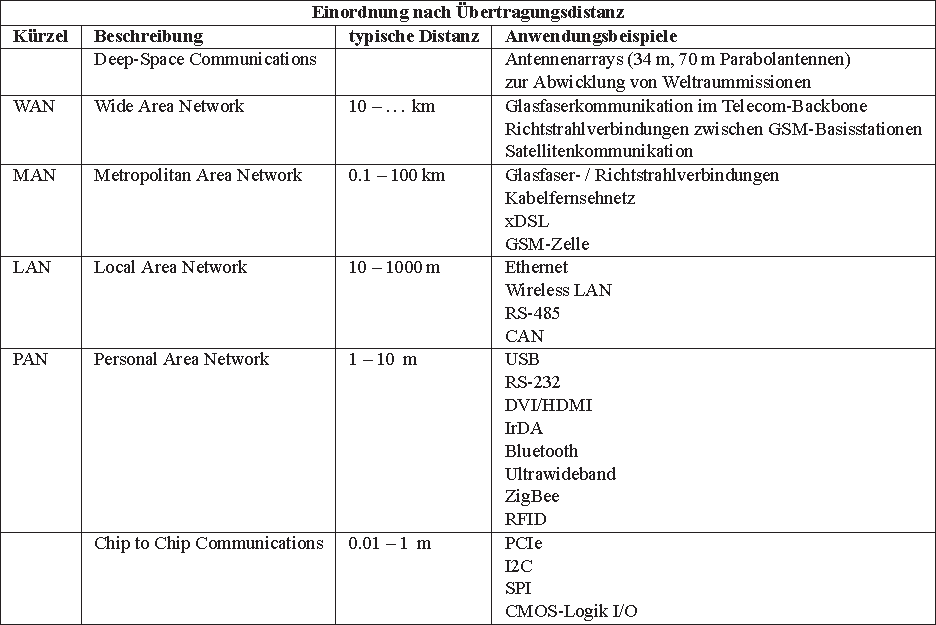
\includegraphics[width=.83\textwidth]{content/02_Klassifizierung/Tabelle1_3.pdf}
\end{table}
\subsection{Klassifizierung nach Zugriffsverfahren S.4}
\begin{table}[H]
	\centering
	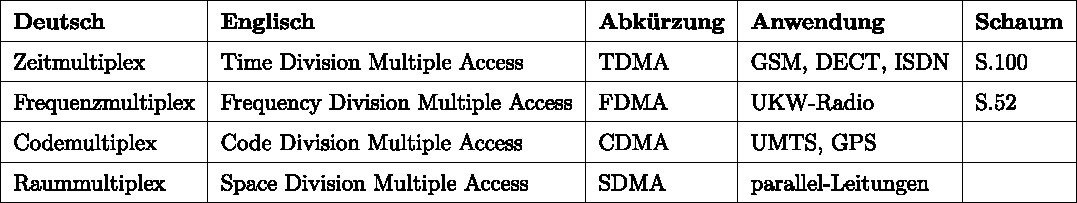
\includegraphics[width=.85\textwidth]{content/02_Klassifizierung/multiplexingverfahren.pdf}
\end{table}
\subsection{Klassifizierung nach Frequenzbereich S.6}
\begin{table}[H]
	\centering
	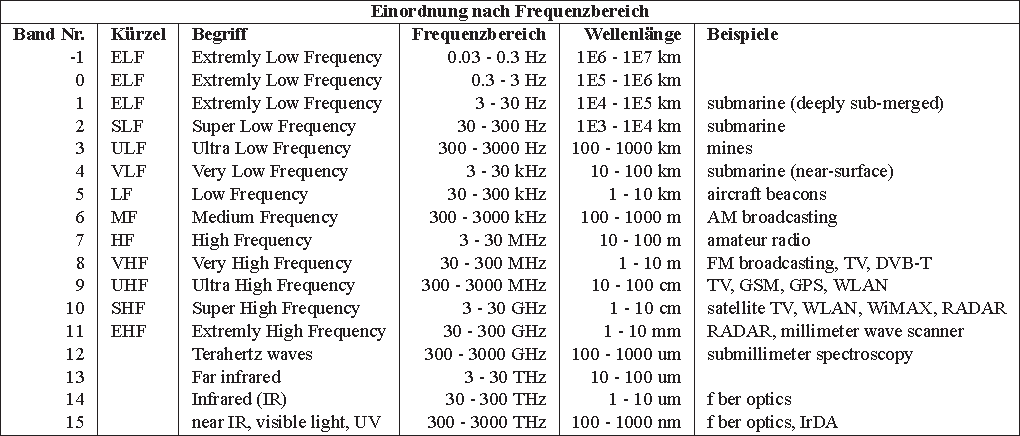
\includegraphics{content/02_Klassifizierung/Tabelle1_5.pdf}
\end{table}
\subsection{Klassifizierung nach Adressierung S.6}
\begin{table}[H]
	\centering
	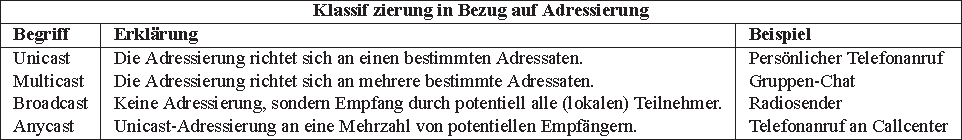
\includegraphics{content/02_Klassifizierung/Tabelle1_6.pdf}
\end{table}


\newpage
% \input{content/02_Signale/02_Signale}
	\section{Signale S.7}
\subsection{Klassifizierung von Signalen S.7}
\begin{table}[H]
	\begin{tabularx}{\textwidth}{|X|X|}
		\hline
		\begin{minipage}{\linewidth}Energiesignal $E=\int_{-\infty}^{\infty}|x(t)|^2 dt < \infty$ \end{minipage}
		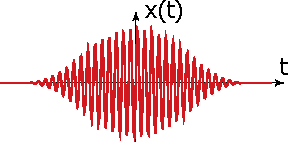
\includegraphics{content/03_Signale/energiesignal.pdf}
		& 
		\begin{minipage}{\linewidth}Leistungssignal $ P=\lim\limits_{T->\infty} \frac{1}{T} \int_{-T/2}^{T/2}|x(t)|^2 dt < \infty$\end{minipage}
		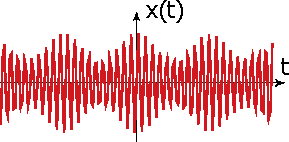
\includegraphics{content/03_Signale/leistungssignal.pdf}
		\\
		\hline
		\\
		\begin{minipage}{\linewidth}aperiodisches Signal $x(t) \neq x(t+n \cdot T)$\end{minipage}
		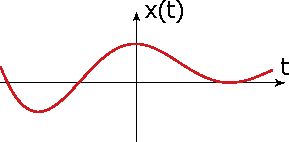
\includegraphics{content/03_Signale/aperiodischessignal.pdf}
		& 
		\begin{minipage}{\linewidth}periodisches Signal$x(t) = x(t+n \cdot T)$\end{minipage}
		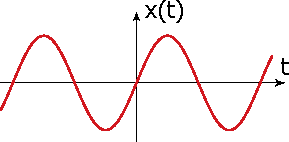
\includegraphics{content/03_Signale/periodischessignal.pdf}
		\\
		\hline
		\\
		\begin{minipage}{\linewidth} deterministisches Signal \\ $x(t) = f(t)$ Verlauf ist bekannt \end{minipage}
		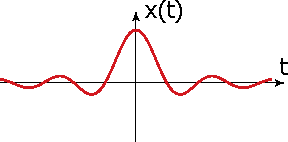
\includegraphics{content/03_Signale/deterministischessignal.pdf}
		&
		\begin{minipage}{\linewidth}{stochastisches Signal: Signalverlauf ist unbekannt bzw. zufällig}\end{minipage}
		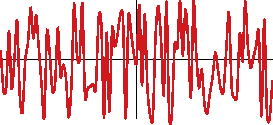
\includegraphics{content/03_Signale/stochastischessignal.pdf}
		\\
		\hline
		\\
		\begin{minipage}{\linewidth} zeitkontinuierliches Signal $x(t)$ ist immer definiert \end{minipage}
		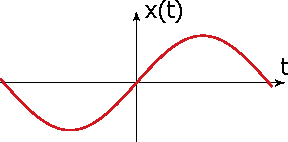
\includegraphics{content/03_Signale/zeitkontinuierlichessignal.pdf}
		&
		\begin{minipage}{\linewidth}zeitdiskretes Signal $x(t)$ ist nur an diskreten Punkten definiert\end{minipage}
		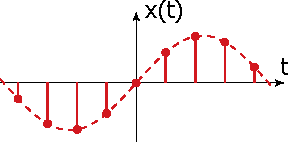
\includegraphics{content/03_Signale/zeitdiskretessignal.pdf}
		\\
		\hline
		\\
		\begin{minipage}{\linewidth}amplitudenkontinuierliches Signal\end{minipage}
		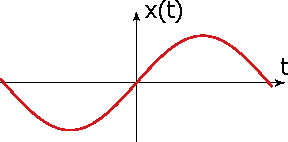
\includegraphics{content/03_Signale/amplitudenkontinuierlichessignal.pdf}
		&\begin{minipage}{\linewidth} quantisiertes Signal \end{minipage}
		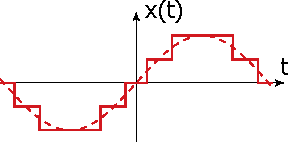
\includegraphics{content/03_Signale/quantisiertessignal.pdf}
		\\
		\hline
		\\
		\begin{minipage}{\linewidth} Zeit- und Amplitudenkontinuierliches Signal (Analog) \end{minipage}
		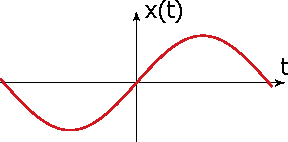
\includegraphics{content/03_Signale/zeitamplitudenkontinuierlichessignal.pdf}
		& \begin{minipage}{\linewidth} Zeitdiskret und Quantisiert \end{minipage}
		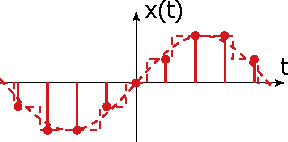
\includegraphics{content/03_Signale/zeitdiskretquantisiert.pdf}
		\\
		\hline
	\end{tabularx}
\end{table}
\newpage
\subsection{Kenngrössen von Signalen S.13}
In der Nachrichtentechnik sind Signale in der Regel \textbf{dimensionslos} und \textbf{normiert}. ($|x(t)| \leq 1$) Die \textbf{momentante Signalleistung} beträgt deshalb: $P_x(t) = |x(t)|^2$
\subsubsection{Mittelwerte}\vspace{-1em}

\begin{table}[H]
	\renewcommand{\arraystretch}{2.2}
	\begin{tabularx}{\textwidth}{X X}
		Linearer zeitlicher Mittelwert
		&
		\begin{minipage}{\linewidth}
		\begin{equation*} x_{avg}=\overline{x}=\lim\limits_{T\rightarrow\infty} \frac{1}{T} \int_{-T/2}^{T/2}x(t)dt \end{equation*}
		\end{minipage}
		\\ \hline 
		Effektivwert (Root Mean Square RMS)
		&
		\begin{minipage}{\linewidth}
		\begin{equation*} x_{RMS}=\sqrt{\overline{P_x}}=\sqrt{\lim\limits_{T\rightarrow\infty} \frac{1}{T} \int_{-T/2}^{T/2}|x(t)|^2 dt} \end{equation*}
		\end{minipage}
		\\ \hline 
		mittlere Leistung
		&
		\begin{minipage}{\linewidth}
			\begin{equation*} \overline{P_x} = \lim\limits_{T\rightarrow\infty} \frac{1}{T}\int_{-T/2}^{T/2} P_x(t)dt \left(= \frac{U_{rms}^2}{R} = I_{rms}^2 \cdot R\right)\end{equation*}
		\end{minipage}
	\end{tabularx}
\end{table}

\subsubsection{Crest Faktor (Scheitelfaktor S. 15)}
Der Crest Faktor gibt das Verhältnis zwischen Spitzenwert $x_p$ und Effektivwert $x_{RMS}$ an. Ist der Crestfaktor bekannt, kann ein Verstärker basierend auf dem Effektivwert des Signals so eingestellt werden, dass ein Übersteuern verhindert wird. Grosses C = viel Amplitude bei wenig Leistung $\rightarrow$ nicht so gut. Für sinusförmige Signale $C = \sqrt{2}$
\begin{equation*}
	C = \frac{x_p}{x_{RMS}} = \frac{max(|x(t)|)}{\sqrt{P_x}}
\end{equation*}

\subsubsection{Logarithmische Beschreibung von Leistungsverhältnissen S. 16}
Leistungen von Signalen werden üblicherweise auf einer logarithmischen Skala (dB) verglichen. \textbf{\color{red}Mit dB werden immer Leistungen verglichen, nicht Amplituden!}
\begin{table}[H]
\centering
\renewcommand{\arraystretch}{1.2}
\begin{tabularx}{\textwidth}{XX}
\begin{minipage}[t]{\linewidth}\centering
Signal to Noise Ratio (SNR)\\[6pt]
$SNR = \dfrac{S}{N} = \dfrac{\text{Signalleistung}}{\text{Rauschleistung}}$
\end{minipage}
&
\begin{minipage}[t]{\linewidth}\centering
Leistungsverhältnis (wo $P_x$ Referenzleistung)\\[6pt]
$k_{dB} = 10 \cdot k_{Bel} = 10 \cdot \log_{10}\!\left(\dfrac{P_y}{P_x}\right)$ \\
$[k_{Bel}] = \text{Bel} \qquad [k_{dB}] = \text{dB}$
\end{minipage}
\end{tabularx}
\end{table}

\begin{minipage}{.4\linewidth}
	\renewcommand{\arraystretch}{2}
	\begin{tabular}{|c|c|c||c|c|c|}
		\hline
		dB & $\dfrac{P_{y}}{P_{x}}$ & $\dfrac{y_{rms}}{x_{rms}}$&dB & $\dfrac{P_{y}}{P_{x}}$ & $\dfrac{y_{rms}}{x_{rms}}$\\
		\hline
		20	&	100	&	10 &-20	& 	$\dfrac{1}{100}$	&	$\dfrac{1}{10}$	\\
		10	&	10	&$\sqrt{10}$& -10	& 	$\dfrac{1}{10}$	&	$\dfrac{1}{\sqrt{10}}$\\
		6	& 	4	&	2	&-6	& 	$\dfrac{1}{4}$	&	$\dfrac{1}{2}$\\
		3	& 	2	&	$\sqrt{2}$ & & &	\\
		0	& 	1	&	1 & -3	&	$\dfrac{1}{2}$	&	$\dfrac{1}{\sqrt{2}}$	\\
		\hline
	\end{tabular}
\end{minipage}
\begin{minipage}{.59\linewidth}
	\begin{equation*}
	10 \cdot \log_{10} \left(\frac{P_y}{P_x}\right) = 10 \cdot \log_{10} \left(\frac{y^2_{RMS}}{x^2_{RMS}}\right) = 20 \cdot \log_{10} \left(\frac{y_{RMS}}{x_{RMS}}\right) 
	\end{equation*}
	\begin{center}
		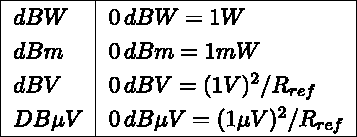
\includegraphics{content/03_Signale/Tabelle2_2.pdf}
	\end{center}
		Bei Spannungspegeln muss Referenzwiderstand berücksichtigt werden. HF üblicherweise 50 $\Omega$, Telefonie 600 $\Omega$
\end{minipage}

\subsubsection{Relative Pegel}
\begin{tabular}{lllr}
	\colorbox{green!30}{\textbf{Spannungspegel}}&  
	$L_u = 20 \cdot \log_{10} \left(\frac{u_x}{u_0}\right)$&
	$U_x = U_0 \cdot 10^{\frac{L}{20}} $ &
	$[L_u] = dB$\\
	
	\textbf{Strompegel}& $L_i  = 20 \cdot \log_{10} \left(\frac{i_x}{i_0}\right)$& $I_x = I_0 \cdot
	10^{\frac{L}{20}} $ & $[L_i] = dB$\\
	
	\colorbox{cyan!30}{\textbf{Leistungspegel}} & $L_P = 10 \cdot \log_{10} \left(\frac{P_x}{P_0}\right)$ & $P_x = P_0 \cdot
	10^{\frac{L}{10}} $ & $[L_P] = dB$ \\
\end{tabular}\renewcommand{\arraystretch}{1}%
\subsubsection{Absolute Pegel}
\begin{tabbing}
	xxxxxxxxxxxxx \= xxxxxxxxxxxxxxxxxxxxxxxxxxxxxxxxxxxxx  \= xxxxxxxxxxxxxxxxxxxxxxx \=\kill
	\colorbox{cyan!30}{\textbf{dBW}} \> Leistungspegel mit Bezugsgrösse $P_0 = $1W \> $\Longrightarrow \: 0 \: dBW = 1W = P_{0_{dBW}}$\\
	\colorbox{cyan!30}{\textbf{dBm}} \> Leistungspegel mit Bezugsgrösse $P_0 = $1mW \> $\Longrightarrow \: 0 \: dBm = 1mW = P_{0_{dBm}}$\\
	\colorbox{green!30}{\textbf{dBV}} \> Spannungspegel mit Bezugsgrösse $U_0 = $1V \> $\Longrightarrow \: 0 \: dBV = P_{0_{dBV}}$\\
	\colorbox{green!30}{\textbf{dB}$\mu$V} \> Spannungspegel mit Bezugsgrösse $U_0 = $1$\mu$V \> $\Longrightarrow \: 0 \: dB \mu V = P_{0_{dB\mu V}}$
\end{tabbing}
\newpage
	\section{Fourierzauberei S.19}
\textbf{Trick 77 $\rightarrow$ Skript S. 253 ff.} Fourier Mit Rechteckfolge, Dreieckfolge, etc. Fouriertrafo einer Fourie Reihe.
\subsection{Fourierreihe S.20}
Fourierreihe funktioniert nur mit \textbf{periodischen} Signalen.
\begin{table}[H]
	\includegraphics{content/04_fourier/fourierreihe.pdf}
\end{table}
Im Skript werden die Fourierkoeffizienten mit $a_n = u_n$ und $b_n = v_n$ bezeichnet! Grund dafür ist die überaus Spannende (und von anderer Literatur abweichende) Bezeichnung des komplexen Koeffizienten (Im Skript: $c_n = a + jb$) Der Zusammenhang in \textbf{Formel 3.12} im Skript S. 22 ist unbedingt zu beachten!

\subsubsection{Koeffizienten berechnen}
$a_0$, $c_0$, $A_0$ sind \textit{Konstanten}, $\omega_1$ ist die
\textit{Grundkreisfrequenz}, $a_n$ und $b_n$ sind die \textit{reellen
	Koeffizienten}, $c_n$ ist der \textit{komplexe Koeffizient}, $A_n$ ist die
\textit{Amplitude} und $\varphi_n$ ist die \textit{Phase}.\\
\begin{center}
\efbox[linecolor=red, leftline=true, rightline=true, topline=true, bottomline=true]{
	\begin{tabular}{p{8cm}p{8cm}}
		$a_n = c_n + \bar{c_n} = 2\Re(c_n) = A_n \cos(\varphi_n)$ &
		$b_n = j(c_n + \bar{c_n}) = -2\Im(c_n) = -A_n \sin(\varphi_n)$ \\
		$c_n = \frac{a_n-jb_n}{2} = \frac{A_n}{2} e^{j\varphi_n} = \frac{\pi}{T}F(j n \omega)$ &
		$c_{-n} = \overline{c_n} = \frac{a_n+jb_n}{2} = \frac{A_n}{2} e^{-j\varphi_n}$ \\
		$A_n = 2|c_n| = \sqrt{a_n^2+b_n^2}$ & $\varphi_n =  \arg(c_n)$ oder unten $\downarrow$\\
\end{tabular}}	
\end{center}
\textbf{Berechnung von $\varphi_n$ aus $a_n$ und $b_n$}\\
\begin{tabular}{p{4cm}p{4cm}p{3cm}p{3.5cm}}
	$a_n> 0:$ & $\varphi_n = -\arctan(\frac{b_n}{a_n})$ &
	$a_n<0:$ &	$\varphi_n = -\arctan(\frac{b_n}{a_n}) + \pi$\\
	$a_n = 0 \wedge b_n > 0:$ &	$\varphi_n = -\frac{\pi}{2}$ &
	$a_n = 0 \wedge b_n < 0:$ &	$\varphi_n = \frac{\pi}{2}$\\
	$a_n = 0 \wedge b_n = 0:$ &	$\varphi_n = \text{nicht definiert}$
\end{tabular}

\subsection{Symmetrie}
Siehe auch Skript Seite 22\\
\begin{tabular}{|p{4.3cm}|p{4.3cm}||p{4.4cm}|p{4.4cm}|}
	\hline
	\textbf{gerade Funktion} & \textbf{ungerade Funktion} &
	\textbf{Halbperiode 1} & \textbf{Halbperiode 2}\\
	\hline
	\includegraphics[width=3cm,trim=0 0 0 -5]{content/04_fourier/gerade_funktion.png}&
	\includegraphics[width=3cm]{content/04_fourier/ungerade_funktion.png}&
	\includegraphics[width=3cm]{content/04_fourier/halbperiode_1.png}&   
	\includegraphics[width=3cm]{content/04_fourier/halbperiode_2.png}\\
	\hline
	Achsen-symmetrisch & Punkt-symmetrisch & & \\			
	$f(-t)=f(t)$ & $f(-t)=-f(t)$ & $f(t)=f(t+\pi)$ & $f(t)=-f(t+\pi)$\\
	\hline
	$b_n=0$ & $a_n=0$ & $a_{2n+1}=0$ & $a_{2n}=0$\\
	$a_n = \frac{4}{T} \int\limits_0^{\frac{T}{2}} f(t) \cdot \cos(k \omega_1
	t) dt$ &
	$b_n =  \frac{4}{T} \int\limits_0^{\frac{T}{2}} f(t) \cdot
	\sin(n \omega_1 t) dt$ &
	$b_{2n+1}=0$ & $b_{2n}=0$\\
	\hline
\end{tabular}

\subsection{Rechtecksignale S.256}
\boxedeq{\begin{split} A_n=\frac{2}{T}\int\limits_{-t_1/2}^{t_1/2}A\cos\left(\frac{2\pi n}{T}t\right)dt= \frac{2A}{\pi n}\sin\left(\frac{\pi t_1}{T}n\right) \end{split}}

Für Verhältnisse $\frac{T}{ggT(t_1,T)}=n\in\mathbb{N}$ verschwinden die
$n.$ Harmonische und deren Vielfache. (ggT = grösster gemeinsamer Teiler, für sehr wenig schlaue: Taschenrechner \textbf{ggT = gcd} ;-))\\
Formel Skript S. 256; $\tau = \frac{t_{1}}{T}$, $t_1$ ist die Einschaltzeit\\
\includegraphics[width=19cm]{content/04_fourier/fourierreihe-rechteck.png}

\subsection{Satz von Parseval S. 23}
Die mittlere Leistung kann auch aus den komplexen Fourierkoeffizienten berechnet werden.
\begin{equation*}
	\overline{P_x} = \frac{1}{T} \int_{T}|x(t)|^2 dt = \sum_{n=-\infty}^{\infty} |c_k|^2 = \sum_{n=-\infty}^{\infty} |\frac{a_n-jb_n}{2}|^2
\end{equation*}
\subsection{Fourier Transformation S. 23}

La trasformata di Fourier mostra \textbf{quali frequenze} ci sono in un segnale
e \textbf{quanto sono forti}.

\[
\underbrace{x(t)}_{\text{segnale nel tempo}}
\quad \circ\!\!-\!\!\bullet \quad
\underbrace{X(\omega)}_{\text{segnale in frequenza}}
\]

\begin{itemize}
  \item $x(t)$: com'è fatto il segnale \textbf{nel tempo} (come lo vedi sull'oscilloscopio).
  \item $X(\omega)$: lo \textbf{spettro}, cioè quanto c'è di ogni frequenza $\omega$ nel segnale
        (come lo vedi sull'analizzatore di spettro).
\end{itemize}

Die Fourier Transformation erweitert die spektrale Analyse auf \textbf{deterministische Energiesignale}. Herleitung siehe Skript.

Damit die Fourier Transformierte existiert muss die Funktion $x(t)$ absolut integrierbar ($\int_{-\infty}^{\infty} |x(t)| dt \leq \infty$) sein, sowie deren Fourier Transformierte $X(\omega)$ (sonst kann man sie nicht mehr zurück transformieren). Ist $f(t)$ eine Linearkombination von absolut integrierbaren Funktionen wie $x(t)$ und die resultierenden $F(\omega)$ von Funktionen wie $X(\omega)$ , dann ist $f(t)$ ebenfalls transformierbar (Linearität).
\begin{table}[H]
	\begin{tabularx}{\textwidth}{X X}
		\begin{minipage}{\linewidth}
			Fouriertransformierte
			\begin{equation*}
				X(\omega) = \int_{-\infty}^{\infty} x(t) \cdot e^{-j\omega t}dt
			\end{equation*}
		\end{minipage}
		&
		\begin{minipage}{\linewidth}
			Rücktransformierte
			\begin{equation*}
				x(t) = \frac{1}{2\pi}\int_{-\infty}^{\infty} X(\omega) \cdot e^{-j\omega t}d\omega
			\end{equation*}
	\end{minipage}
	\end{tabularx}
\end{table}

\subsubsection{Wichtige Formel}
\[e^{\pm j\omega t} = \cos(\omega t) \pm j\sin(\omega t) \qquad 
\cos(\omega t) = \frac{e^{j\omega t} + e^{-j\omega t}}{2} \qquad
\sin(\omega t) = \frac{e^{j\omega t} - e^{-j\omega t}}{2j}\]


\subsubsection{Eigenschaften der Fourier Transformation S.24}
\renewcommand{\arraystretch}{2}
\begin{tabular}{|p{2.5cm}|p{6cm}|p{8.5cm}|}
	\hline
	\multicolumn{2}{|l}{Linearität} & $\alpha\cdot f(t) + \beta\cdot g(t) \; \laplace \; \alpha\cdot F(\omega) +\beta\cdot G(\omega) \qquad (\alpha, \beta \in \mathbb{C})$  \\ 
	\hline
	\multicolumn{2}{|l}{Zeitumkehrung (Spiegelung an der Y-Achse)} & $f(-t) \; \laplace \; F(-\omega)$ \\
	\hline
	\multicolumn{2}{|l}{"Ahnlichkeit / (Zeitskalierung)}             &      		$\begin{aligned}f(\alpha t) \; &\laplace \; \frac{1}{|\alpha|}F \left (\frac{\omega}{\alpha} \right)
		\quad\alpha \in\mathbb{R}\setminus \{0\}\\
		F(\alpha\omega) \; &\Laplace \; f\left(\frac{t}{\alpha}\right)\end{aligned}$\\ 
	\hline
	\multicolumn{2}{|l}{Vertauschungssatz (Dualität)}              & 
	\begin{math}
		\begin{aligned}
			f(t) \; &\laplace \; F(\omega)\nonumber \\ 
			F(t) \; &\laplace \; 2\pi \cdot f(-\omega)
		\end{aligned}
	\end{math}\\ 
	\hline
	\hline
	\multirow{2}{*}{Verschiebung} & Zeitbereich & $f(t\pm t_0) \; \laplace \; F(\omega)e^{\pm j\omega t_0}$ \\ 
	\cline{2-3} 
	& Frequenzbereich (Modulationstheorem) & $f(t)e^{\pm j\omega_0 t} \; \laplace \; F(\omega\mp\omega_0)$ \\ 
	\hline
	\hline
	\multirow{2}{*}{Faltung} & Zeitbereich & $f(t) \ast g(t) = \int\limits_{-\infty}^{\infty} f(\tau)g(t-\tau)d\tau \; \laplace \;
	F(\omega) \cdot G(\omega)$ \\ 
	\cline{2-3} 
	& Frequenzbereich & $f(t) \cdot g(t) \; \laplace \; \frac{1}{2\pi}F(\omega) \ast G(\omega)$ \\ 
	\hline
	\hline
	\multirow{2}{*}{Ableitung} & Zeitbereich & $\frac{\partial^n f(t)}{\partial t^n} \; \laplace \; (j\omega)^n F(\omega) \qquad (n \in \mathbb{N}_0)$ \\ 
	\cline{2-3} 
	& Frequenzbereich &  $t^n f(t) \; \laplace \; j^n \frac{\partial F(\omega)}{\partial \omega^n}$\\ 
	\hline
	\hline
	\multicolumn{2}{|l}{Integration im Zeitbereich} & $\int\limits_{-\infty}^{t}f(\tau)d\tau \; \laplace \;
	\frac{F(\omega)}{j\omega}+F(0)\pi\delta(\omega)$\\ 
	\hline
	\hline
	\multicolumn{2}{|l}{Modulation} & 
	\begin{math}
		\begin{aligned}
			\cos(\alpha t) \cdot f(t)  \; &\laplace \;  \frac{1}{2}\cdot
			\left[F(\omega-\alpha) + F(\omega+\alpha)\right]\\
			\sin(\alpha t) \cdot f(t) \; &\laplace \; \frac{1}{2j}\cdot \left[F(\omega-\alpha) - F(\omega+\alpha)\right]
		\end{aligned}
	\end{math}	\\ 
	\hline
	\hline
	\multirow{2}{*}{Theorem} & Parseval's & 			 			$\int\limits_{-\infty}^{\infty}f(t)g^{\ast}(t)dt = \frac{1}{2\pi}
	\int\limits_{-\infty}^{\infty}F(\omega)G^{\ast}(\omega)d\omega$\\ 
	\cline{2-3} 
	& Bessel's & $\int\limits_{-\infty}^{\infty}|f(t)|^2 dt = \frac{1}{2\pi}
	\int\limits_{-\infty}^{\infty}|F(\omega)|^2 d\omega$ \\ 
	\hline
	\hline
	\multicolumn{2}{|l}{Anfangswerte} & 
	\begin{math}
		\begin{aligned}
			f(0)&=\frac{1}{2\pi}\int\limits_{-\infty}^{\infty}F(\omega)d\omega
			\hspace*{1cm}\\
			F(0)&=\int\limits_{-\infty}^{\infty}f(t)dt
		\end{aligned}
	\end{math} \\
	\hline
	\hline
	\multicolumn{2}{|l}{\begin{minipage}{.5\linewidth}unendlich lange Folge von $\delta$-Impulsen (im Zeit und Frequenzbereich)\end{minipage}} 
	& $\sum\limits_{n=-\infty}^{\infty} \delta(t-n\cdot t_0) \; \laplace \;
	\sum\limits_{n=-\infty}^{\infty} \frac{2\pi}{t_0}\cdot\delta\left(\omega-n\cdot
	\frac{2\pi}{t_0}\right)$ \\ 
	\hline
\end{tabular}

\subsubsection{Wichtige Fourier-Korrespondenzen}
\begin{tabular}{|l|c|c|}
\hline
\textbf{Funktion} & $\boldsymbol{x(t)}$ & $\boldsymbol{X(\omega)}$ \\
\hline
Dirac-Impuls & $\delta(t)$ & $1$ \\
\hline
Verschobener Dirac & $\delta(t-t_0)$ & $e^{-j\omega t_0}$ \\
\hline
Konstante & $1$ & $2\pi\,\delta(\omega)$ \\
\hline
Komplexe Exponentialfunktion & $e^{j\omega_0 t}$ & $2\pi\,\delta(\omega-\omega_0)$ \\
\hline
Cosinus & $\cos(\omega_0 t)$ & $\pi\left[\delta(\omega-\omega_0)+\delta(\omega+\omega_0)\right]$ \\
\hline
Sinus & $\sin(\omega_0 t)$ & $-j\pi\left[\delta(\omega-\omega_0)-\delta(\omega+\omega_0)\right]$ \\
\hline
Sprungfunktion & $u(t)$ & $\pi\,\delta(\omega)+\dfrac{1}{j\omega}$ \\
\hline
Signumfunktion & $\mathrm{sgn}(t)$ & $\dfrac{2}{j\omega}$ \\
\hline
Rechteckimpuls (Breite $2a$) & $p_a(t)$ & $\dfrac{2\sin(a\omega)}{\omega}$ \\
\hline
Rechteckimpuls (Breite $\tau$, Höhe $A$) & $A\cdot\mathrm{rect}\!\left(\dfrac{t}{\tau}\right)$ & $A\tau\cdot\dfrac{\sin(\omega\tau/2)}{\omega\tau/2}$ \\
\hline
Dreieckimpuls (Basis $2a$) & $\Lambda_a(t)$ & $\dfrac{4\sin^2(a\omega/2)}{a\,\omega^2} = a\left[\dfrac{\sin(a\omega/2)}{a\omega/2}\right]^2$ \\
\hline
Sincfunktion & $\mathrm{sinc}_a(t)=\dfrac{\sin(at)}{t}$ & $\pi\,p_a(\omega)$ \\
\hline
Sinc$^2$-Funktion & $\dfrac{\sin^2(at/2)}{t^2}$ & $\dfrac{\pi a}{2}\,\Lambda_a(\omega)$ \\
\hline
Einseitige Exponentialfunktion & $e^{-at}\,u(t),\ a>0$ & $\dfrac{1}{a+j\omega}$ \\
\hline
 & $t\,e^{-at}\,u(t),\ a>0$ & $\dfrac{1}{(a+j\omega)^2}$ \\
\hline
Zweiseitige Exponentialfunktion & $e^{-a|t|},\ a>0$ & $\dfrac{2a}{a^2+\omega^2}$ \\
\hline
Gedämpfter Cosinus & $e^{-at}\cos(\omega_0 t)\,u(t)$ & $\dfrac{a+j\omega}{(a+j\omega)^2+\omega_0^2}$ \\
\hline
Gedämpfter Sinus & $e^{-at}\sin(\omega_0 t)\,u(t)$ & $\dfrac{\omega_0}{(a+j\omega)^2+\omega_0^2}$ \\
\hline
Gaussimpuls & $e^{-at^2},\ a>0$ & $\sqrt{\dfrac{\pi}{a}}\;e^{-\omega^2/(4a)}$ \\
\hline
\end{tabular}
\renewcommand{\arraystretch}{\arraystretchOriginal}
\medbreak

\begin{minipage}{8cm}
	Periodische Signale\vspace{-1em}
	\boxedeq{%
	\sum_{n=-\infty}^{\infty}	c_n \cdot e^{jn\omega_0t} \;\; \Laplace \;\; 2\pi \sum_{n=-\infty}^{\infty} c_n \delta(\omega - n\omega_0)
	}
\end{minipage}
\medbreak

\begin{minipage}{15cm}
	Spektrum Einton Winkelmodulation\vspace{-1em}
	\boxedeq{%
	\sum_{n=-\infty}^{\infty} c_n \cdot cos((\omega_c + n\omega_m) \cdot t) \;\; \Laplace \;\;
	\sum_{n=-\infty}^{\infty}c_n\pi(\delta(\omega - (\omega_c+n\omega_m))+\delta(\omega+(\omega_c+n\omega_m)))
	}
\end{minipage}
\medbreak

Für weitere Korrespondenzpaare siehe Skript Seite 28 und \textbf{Seite 253 ff}.


\newpage	
	\section{LTI-Systeme (S.29)}
\begin{list}{$\bullet$}{\setlength{\itemsep}{0cm} \setlength{\parsep}{0cm} \setlength{\topsep}{0cm}} 
	\item Lineare Systeme sind durch die Antworten auf die
	Basissignale bestimmt.
	\item Basissignale müssen linear unabhängig voneinander sein
	\item Alle Eingangs-Funktionen müssen durch eine Linearkombination der
	Basissignale darstellbar sein.\\ $\Rightarrow$ \textbf{Periode des Eingangssignals =	Anzahl Basissignale}
\end{list}
	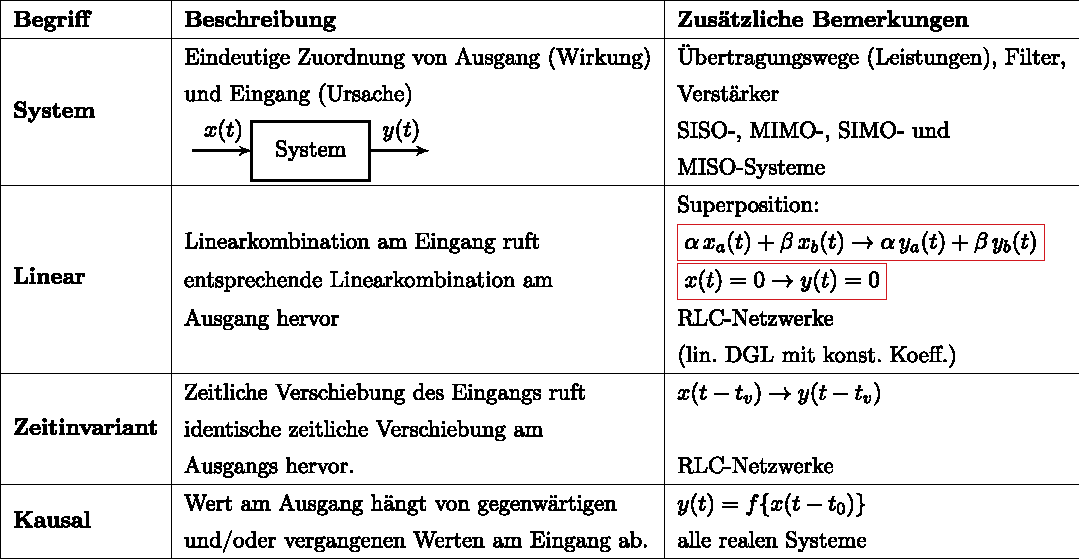
\includegraphics[width=0.9\textwidth]{content/05_LTI/tab_LTI.pdf}

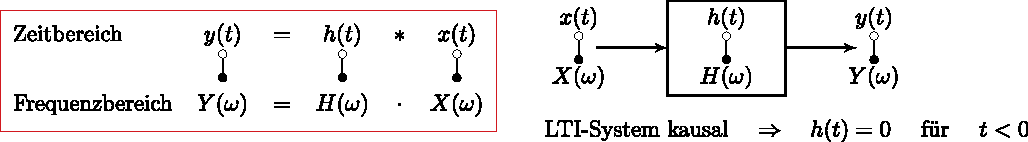
\includegraphics{content/05_LTI/Faltung_System.pdf}
\subsection{Verzerrungsfreies LTI-System S.33}
\vspace{.03cm}
Ein LTI System ist verzerrungsfrei wenn \efbox[linecolor=red]{$H(\omega) = k_a \cdot e^{-j\omega t_d}$} gilt. Der Amplitudengang muss konstant sein ($H(\omega) = k_a$) und der Phasengang eine lineare Funktion von $f$ bzw. $\omega$ sein. Für kausale Systeme muss \textbf{Verzögerung} $t_d > 0$ sein und damit fällt der Phasengang mit steigender Frequenz linear ab: $\varphi(\omega) = -t_d \cdot \omega$

\subsection{Dirac Impuls (Stösschen) S.30}
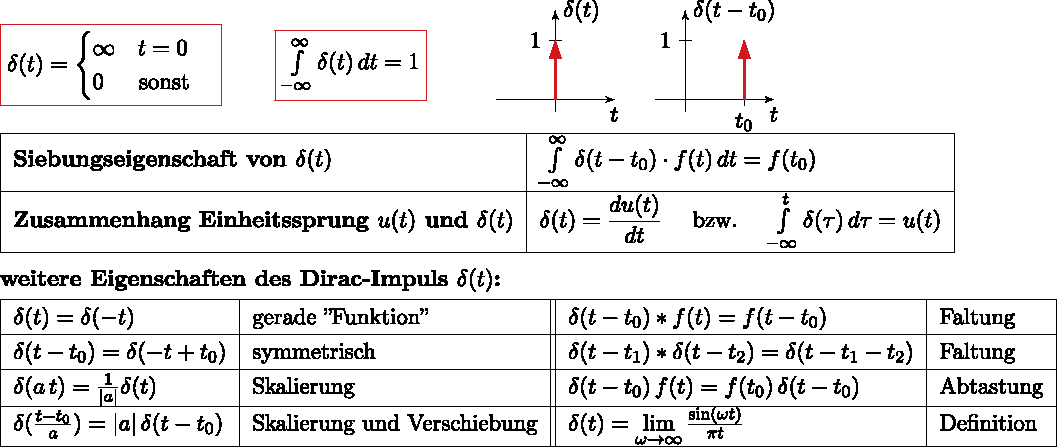
\includegraphics[width=.95\linewidth]{content/05_LTI/stoesschen.pdf}

\subsection{Signalmanipulationen}
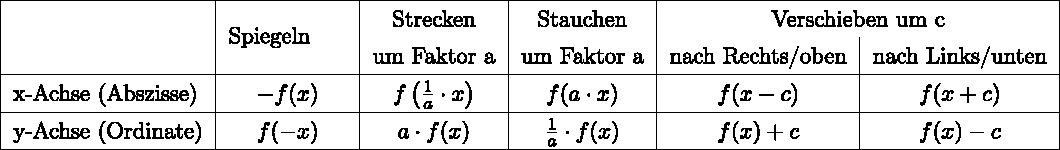
\includegraphics[width=\textwidth]{content/05_LTI/signalmanipulation.pdf}

\subsection{Grundlegende Funktionen S.30}
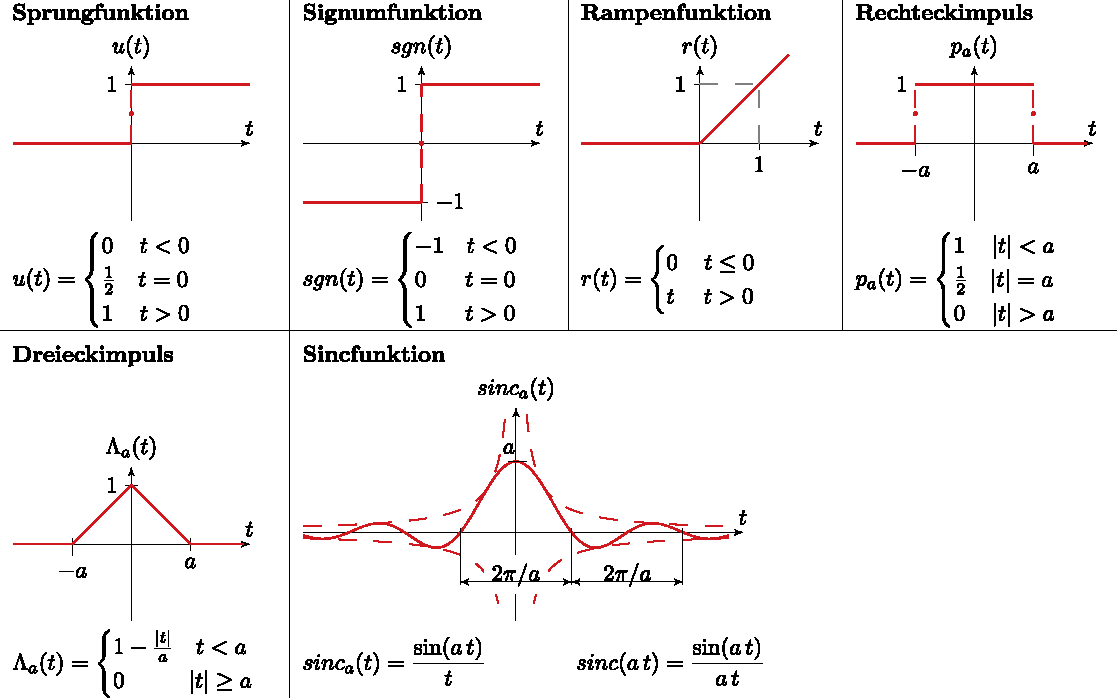
\includegraphics[width=\textwidth]{content/05_LTI/grundlegende_funktionen.pdf}

\subsection{Filtereigenschaften von LTI Systemen S.33}

\begin{minipage}{.4\linewidth}
	\begin{center}
		\begin{tabular}{|c|c|c|}
			\hline
			Tiefpass & Lowpass Filter & LPF \\
			\hline
			Hochpass & Highpass Filter & HPF \\
			\hline
			Bandpass & Bandpass Filter & BPF \\
			\hline
			Bandsperre & Bandstop Filter & BSF \\
			\hline
		\end{tabular}
	\end{center}
\end{minipage}
\begin{minipage}{.6\linewidth}
	Ideale Filter sind \textbf{akausal} und deshalb \textbf{nicht realisierbar}. Reale Filter stellen einen Kompromiss dar:
	\begin{list}{$\bullet$}{\setlength{\itemsep}{0cm} \setlength{\parsep}{0cm} \setlength{\topsep}{0cm}} 
		\item Filterflankensteilheit
		\item Dämpfung im Sperrbereich
		\item Flachem Frequenzgang im Durchlassbereich
		\item Linearität des Phasengangs
	\end{list}
\end{minipage}

\subsubsection{Bandbreite}
Die Bandbreite ist nur für \textbf{Tiefpass und Bandpassfilter} definiert. Bei realen Filtern wird üblicherweise die \textbf{\qty{3}{\dB} Eckfrequenz} angenommen, dabei erreicht die Amplitudendämpfung einen Wert von $k=\frac{1}{\sqrt{2}}$

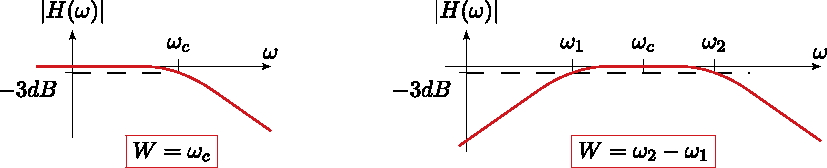
\includegraphics{content/05_LTI/tiefbandpassbandbreite.pdf}

\subsection{Quadraturfilter, Hilberttransformation S. 37}
Der Quadraturfilter ist ein Allpassfilter, dieser lässt die Amplitude unverändert und dreht nur die Phase um eine viertel Periode $-\frac{\pi}{2}$. Es resultiert eine grosse Verzögerung für tieffrequente Anteile und eine kleine für hochfrequente Anteile.

\vspace{.03cm}
\begin{minipage}{.5\linewidth}
\efbox[linecolor=red]{$H(\omega) = -j \cdot sgn(\omega) = \left\{
	\begin{matrix}
		e^{-j\pi /2} \;\; \omega > 0\\
		e^{+j\pi /2} \;\; \omega < 0
	\end{matrix}
	\right.$}
\end{minipage}
\begin{minipage}{.5\linewidth}
	\vspace{.03cm}
	\hspace{.01cm}
	\efbox[linecolor=red]{$h(t) = \frac{1}{\pi \cdot t}$}
\end{minipage}


	\section{Analoge Modulationsarten S. 39}
Bei der Modulation wird ein Trägersignal (z.B. Sinus oder Rechtecksignal) von einem Nachrichtensignal $m(t)$ geformt. Das Nachrichtensignal soll von seinem Basisband in das Übertragungsband des Trägersignals gebracht werden.

Das \textbf{Basisband} bezeichnet den Ursprünglichen Frequenzbereich des Nachrichtensignals. Typischerweise von \qty{0}{\Hz} bis zur \textbf{Bandbreite} $B_m$. Das Übertragungsband liegt meist deutlich darüber. Im Übertragungsband handelt es sich üblicherweise um \textbf{Bandpassignale}

\begin{minipage}{.4\textwidth}
	\textbf{Modulation Sinusträger}
	
	\begin{list}{$\bullet$}{\setlength{\itemsep}{0cm} \setlength{\parsep}{0cm} \setlength{\topsep}{0cm}} 
	\item Amplitudenmodulation (AM)
	\item Frequenzmodulation (FM)
	\item Phasenmodulation (PM)
	\item Hybride Verfahren (z.B. QAM)
	\end{list}
\end{minipage}
\begin{minipage}{.6\textwidth}
	\textbf{Modulation Rechteckträger}
	
	\begin{list}{$\bullet$}{\setlength{\itemsep}{0cm} \setlength{\parsep}{0cm} \setlength{\topsep}{0cm}} 
		\item Pulsamplitudenmodulation (PAM) $x_{PAM}(t)$ mit $m(t)~A_c(t)$
		\item Pulsweitenmodulation (PWM) $x_{PWM}(t)$ mit $m(t) ~\tau(t)$
		\item Pulspositionsmodulation (PPM) $x_{PPM}(t)$ mit $m(t) ~ \Delta T(t)$
		\item Pulsfrequenzmodulation (PFM) $x_{PFM}(t)$ mit $m(t)~f_p(t)$
	\end{list}
\end{minipage}

\subsection{Amplitudenmodulation (AM) S. 44}
Bei der Amplitudenmodulation formt das Nachrichtensignal die Amplitude des Trägersignals (carrier).

\vspace{.1cm}
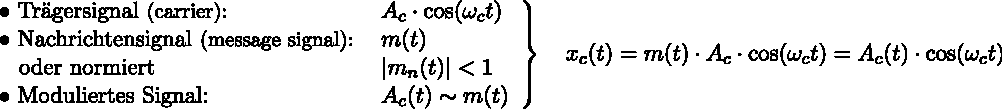
\includegraphics{content/06_amplitudenmodulation/AMbasic.pdf}

\vspace{.1cm}
$\rightarrow$ \textbf{Euler}:\hspace{.1cm} \efbox[linecolor=red]{$
		sin(t) = \frac{1}{2j}\cdot (e^{jt} - e^{.jt}) \;\;\;\;
		cos(t) = \frac{1}{2}\cdot (e^{jt} + e^{.jt})$}

\subsubsection{Frequenzmischer, Frequenzmultiplex S. 46}
Die Multiplikation des Signals $x(t)$ mit dem Träger $cos(\omega_0t)$ verschiebt das Spektrum nach $+/- \omega_0$.

\includegraphics{content/06_amplitudenmodulation/Frequenzmischer.pdf}

\newpage
\subsubsection{Gewöhnliche Amplitudenmodulation S. 44}
Bei der gewöhnlichen AM wird das Nachrichtensignal $m(t)$ mit einem DC offset angehoben um einen Nulldurchgang von $m(t)$ zu verhindern:\hspace{0.01cm} \vspace{.05cm} \efbox[linecolor=red]{$x_{AM}(t) = A_c \cdot (1+\mu \cdot m_n(t)) \cdot cos(\omega_c t)$ \;\; mit $|m(t)| \leq 1$ und Modulationsgrad $\mu$} \\
\textbf{Aufgrund des DC-Anteils ist die gewöhnliche AM nicht linear und nicht zeitinvariant!}

\paragraph{Modulation}
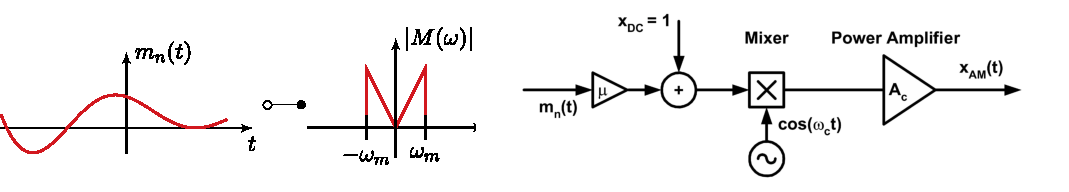
\includegraphics{content/06_amplitudenmodulation/AM_grafik.pdf}

\boxedeq{\begin{split}
		x_{_{AM}}(t) = (1 + \mu \cdot m_n(t)) \cdot A_C \cdot  \cos(\omega_c t)
		\; \;\;\; \laplace \;\;\; \; X_{AM}(\omega) = \frac{\mu A_c}{2}  (M(\omega - \omega_c) + 
		M(\omega + \omega_c)) \\ + \pi A_c [\delta (\omega - \omega_c) + 
		\delta (\omega + \omega_c)] \end{split}} \\

\begin{table}[H]
	\begin{tabularx}{\linewidth}{X X X}
		\begin{minipage}{\linewidth}
		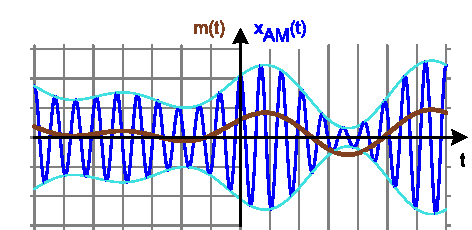
\includegraphics[width=\linewidth]{content/06_amplitudenmodulation/abbildung5_10.pdf}
		\end{minipage}
		&
		\begin{minipage}{\linewidth}
		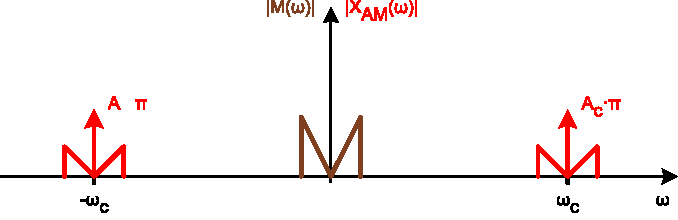
\includegraphics[width=\linewidth]{content/06_amplitudenmodulation/abbildung5_12.pdf}
		\end{minipage}
		&
		\begin{minipage}{1.05\linewidth}
			\textbf{DC-Anteil:} bewirkt, dass Carrier im Frequenzbereich nicht verschwindet \\
			\textbf{Modulationsindex $\mu$ :} $0 < \mu < 1$ \\
			$\mu > 1$ $\rightarrow$ Übermodulation \\
			 \efbox[linecolor=red]{$\mu = \frac{\max|x_{AM}|-min|x_{AM}|}{\max|x_{AM}|+min|x_{AM}|} $}
		\end{minipage}
	\end{tabularx}
\end{table}

\begin{tabular}{m{10cm} m{5cm}}
\paragraph{Demodulation}\mbox{ }
		\vspace{.2cm}
	
	\begin{list}{$\bullet$}{\setlength{\itemsep}{0cm} \setlength{\parsep}{0cm} 	\setlength{\topsep}{0cm}} 
		\item Hüllkurvendetektor (Envelope Detector) S.45
		\item Kohärente Produktdemodulation (siehe DSB-SC)
	\end{list}
\vspace{.5cm}
	\textbf{Bedingungen für Envelop-Demodulation}
	\vspace{.2cm}
	
	\begin{minipage}{\linewidth}
	\begin{list}{$\bullet$}{\setlength{\itemsep}{0cm} \setlength{\parsep}{0cm} 	\setlength{\topsep}{0cm}} 
		\item Umhüllende darf \textbf{nicht unter Null} fallen
		\item Modulationsindex $0 < \mu < 1$, bei Übermodulation fällt Umhüllende unter Null
		\item optimale Zeitkonstante des Hüllkurvendetektors \\
		$B_m < \frac{1}{RC} << f_c $ mit $B_m$: Bandbreite von $m(t)$
	\end{list}
	\end{minipage}
	
	&
	\begin{minipage}{0.4\linewidth}
		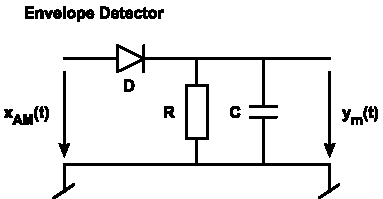
\includegraphics{content/06_amplitudenmodulation/abbildung5_9.pdf}
		
		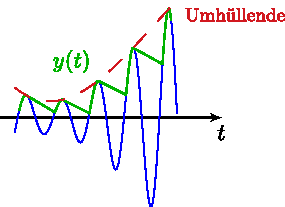
\includegraphics{content/06_amplitudenmodulation/envelope_graph.pdf}
	\end{minipage}

\end{tabular}

\newpage
\paragraph{Äquivalente Basisbanddarstellung der gewöhnlichen AM S. 47}
Vereinfacht gesagt wird die \textbf{Schwingung des Trägeres einfach weggelassen}, die Amplitude $A_c$ aber nicht.
\vspace{.3cm}

\begin{tabular}{m{.4\textwidth} m{.25\textwidth}}
	\begin{minipage}{\linewidth}
		Für Cosinusträger resultiert: \\
		\vspace{.5cm}
		\hspace{.3cm}\efbox[linecolor=red]{$x_{eq}(t) = A_c \cdot (1+ \mu m_n(t))$} \\
		In Abbildung rechts:
		$A_c = 1$, $\mu = \qty{25}{\%}$ (Länge des roten Strichs geht von 0.75 bis 1.25)
	\end{minipage}
	 & 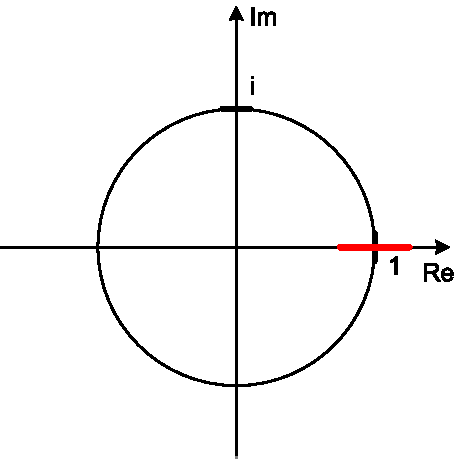
\includegraphics[width=.9\linewidth]{content/06_amplitudenmodulation/eqBaseCosine.pdf} \\ 
	 \begin{minipage}{\linewidth}
	 	Für Sinusträger muss wegen Euler noch ein $-j$ beibehalten werden! \\
	 	\vspace{.3cm}
	 	\hspace{.2cm}\efbox[linecolor=red]{$x_{eq}(t) = -j \cdot A_c \cdot (1+ \mu m_n(t))$}\\
	 	$A_c = 1$, $\mu = \qty{50}{\%}$ (Länge des roten Strichs geht von 0.50j bis 1.5j)
	 \end{minipage}
 & 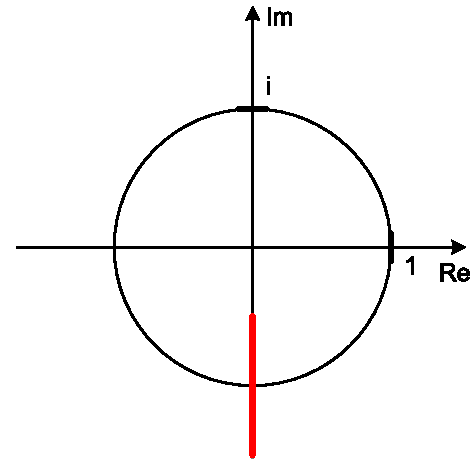
\includegraphics[width=.9\linewidth]{content/06_amplitudenmodulation/eqBaseSine.pdf}
\end{tabular}
\begin{minipage}{.3\textwidth}
	\begin{center}
		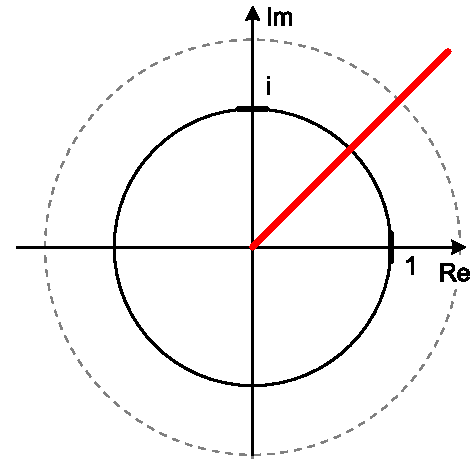
\includegraphics[width=.75\linewidth]{content/06_amplitudenmodulation/egBasePhaseShift.pdf}
	\end{center}
Cosinusträger mit Phasenverschobenem Trägersignal \\
\begin{center}
	\hspace{.1cm} \efbox[linecolor=red]{$x_{eq}(t) = \frac{1+j}{\sqrt{2}} \cdot A_c \cdot (1+\mu m_n(t))$}
\end{center}
$A_c=1$ \\
$\mu = \qty{100}{\%}$
\end{minipage}

\paragraph{Leistungseffizienz der gewöhnlichen AM S. 49}
Unter der Effizienz $\eta$ der gewöhnlichen AM versteht man das Verhältnis von Signalleistung $P_s$ der \textbf{beiden Seitenbänder} zur Gesamtleistung $P_t$ des AM-Signals.
\begin{equation*}
	P_c = \frac{A_c^2}{2} \;\; \text{und} \;\; P_t = \frac{A_c^2}{2} + \frac{A_c^2 \mu^2P_m}{2} \rightarrow \eta = \frac{P_s}{P_t} = \frac{P_t - P_c}{P_t} = \frac{\mu^2P_m}{1+\mu^2P_m} = \frac{(\frac{\mu}{C})^2}{1+(\frac{\mu}{C})^2} = \frac{\mu^2 \cdot m^2_{rms}}{1+\mu^2 \cdot m^2_{rms}}
\end{equation*}
Die maximal mögliche Effizienz ($\mu = \qty{100}{\%}$) beträgt \qty{33}{\%}. Bei $\mu = \qty{50}{\%}$ sind noch \qty{11.1}{\%} möglich.

\subsubsection{DSB-SC - Zweiseitenbandamplitudenmodulation ohne Träger S. 51}
Double-Sideband Suppressed-Carrier Modulation
\paragraph{Modulation}

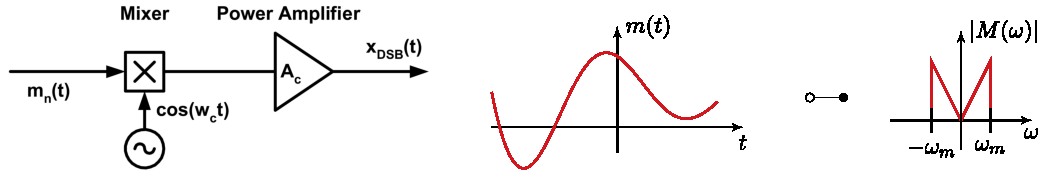
\includegraphics{content/06_amplitudenmodulation/DCBmodulation_grafik.pdf}
\begin{table}[H]
	\begin{tabularx}{\linewidth}{X X X}
		\begin{minipage}{\linewidth}
			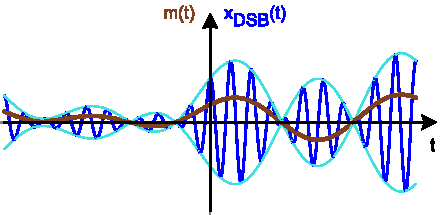
\includegraphics[width=\linewidth]{content/06_amplitudenmodulation/abbildung5_17.pdf}
		\end{minipage}
		&
		\begin{minipage}{\linewidth}
			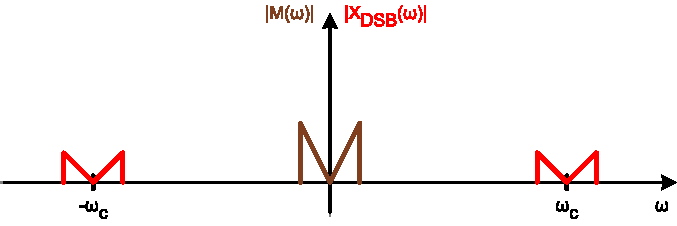
\includegraphics[width=\linewidth]{content/06_amplitudenmodulation/abbildung5_18.pdf}
		\end{minipage}
		&
		\begin{minipage}{1\linewidth}
			\textbf{Bandbreite:} \\$X(\omega) = 2 \cdot \text{ Bandbreite } M(\omega)$ \\
			\textbf{Amplitude:} \\$1/2 \text{ Amplitude } M(\omega)$\\
			(wenn $A_c = 1$)
		\end{minipage}
	\end{tabularx}
\end{table}
\textbf{DSB-SC ist linear, aber nicht zeitinvariant!} Trotzdem wird AM oft als lineare Modulation bezeichnet. Weil bei DSB-C und gewöhnlicher AM das Spektrum nur verschoben wird.

\paragraph{Demodulation S. 53}
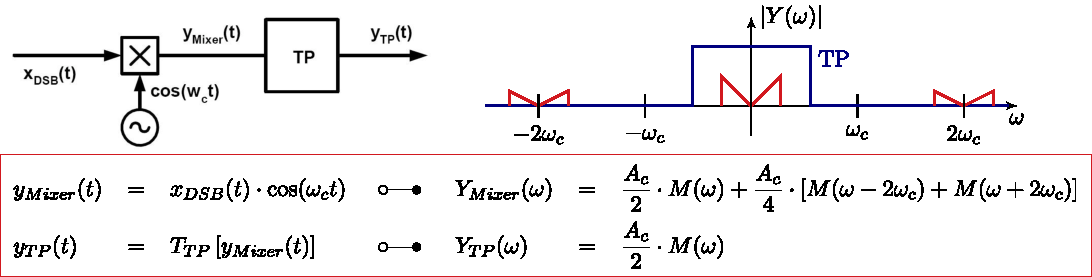
\includegraphics{content/06_amplitudenmodulation/DSB_SC_demodulation.pdf}

Das DSB-Signal wird mit einem sogenannten \textbf{synchronen Demodulator} oder \textbf{kohärenten Demodulator} zurückgewonnen. Weicht die \textbf{Frequenz oder die Phase} des demodulierten, lokalen Trägers von dem, des ursprünglichen Trägers ab, so ergibt sich eine \textbf{Abschwächung im demodulierten Signal}.

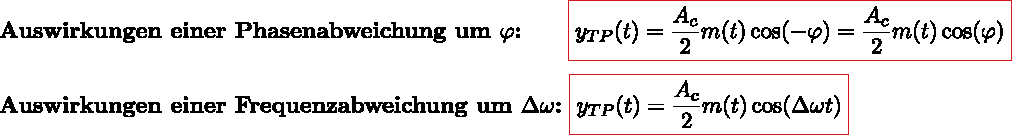
\includegraphics{content/06_amplitudenmodulation/demod_abweichung.pdf}

\subsubsection{Einseitenbandamplitudenmodulation (SSB) S. 53}
Bei der SSB Modulation wird \textbf{nur ein Seitenband übertragen}. Die Implementierung gegenüber gewöhnlicher AM und DSB ist komplexer.
\paragraph{Modulation - Filtermethode S. 54}
Mit einem Bandpassfilter kann entweder das USB (upper side band) oder das LSB (lower side band) unterdrückt werden um ein Einseitenband-Signal zu erhalten. Allerdings stellt dies \textbf{hohe Anforderungen an die Flankensteilheit} des Filters.

\paragraph{Modulation - Phasenmethode}
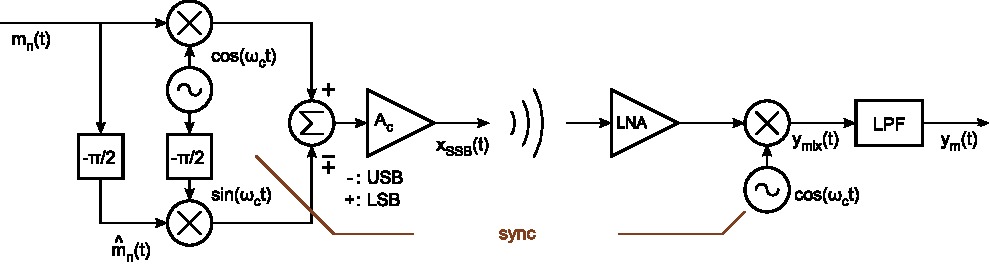
\includegraphics{content/06_amplitudenmodulation/abbildung5_23.pdf}
\begin{table}[H]
	\begin{tabularx}{\linewidth}{X X}
		\begin{minipage}{\linewidth}
			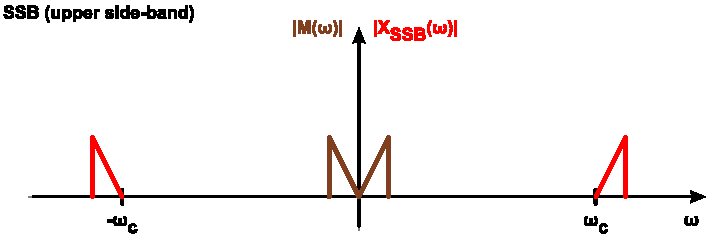
\includegraphics[width=\linewidth]{content/06_amplitudenmodulation/abbildung5_22_1.pdf}
		\end{minipage}
	&
	\begin{minipage}{\linewidth}
		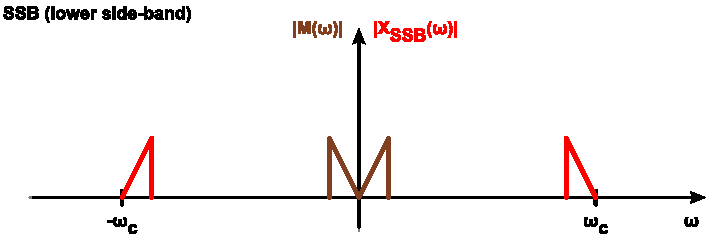
\includegraphics[width=\linewidth]{content/06_amplitudenmodulation/abbildung5_22_2.pdf}
	\end{minipage}
	\end{tabularx}
\end{table}
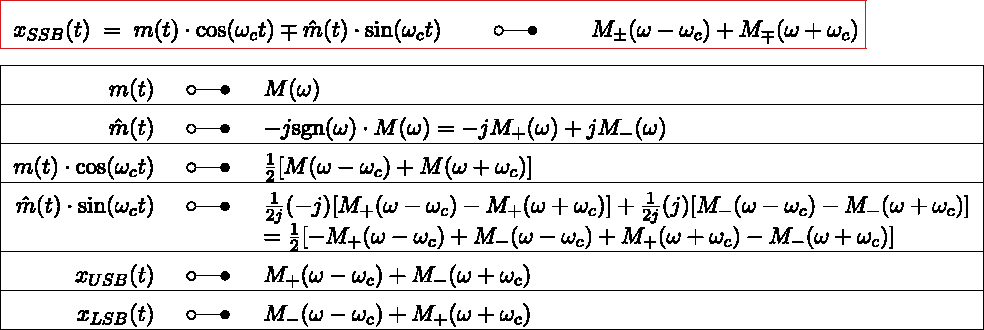
\includegraphics{content/06_amplitudenmodulation/SSB_phasenmethode.pdf}

\paragraph{Demodulation S. 56}
\textbf{Kohärente Demodulation ist erforderlich!}

\includegraphics{content/06_amplitudenmodulation/SSB_demod.pdf}

\subsubsection{Restseitenband-Amplitudenmodulation (VSB) S. 57}
Siehe auch Folie 23 NaT1\underline{ }3c; Restseitenband-AM ist ein Kompromiss zwischen:
\begin{list}{$\bullet$}{\setlength{\itemsep}{0cm} \setlength{\parsep}{0cm} 	\setlength{\topsep}{0cm}} 
	\item Bandbreiteneffizienz von SSB (1.25 x Bandbreite von SSB)
	\item Einfacher technischer Realisierung von DSB (keine extremen Anforderungen an Filtersteilheit)
\end{list}
\paragraph{Modulation}
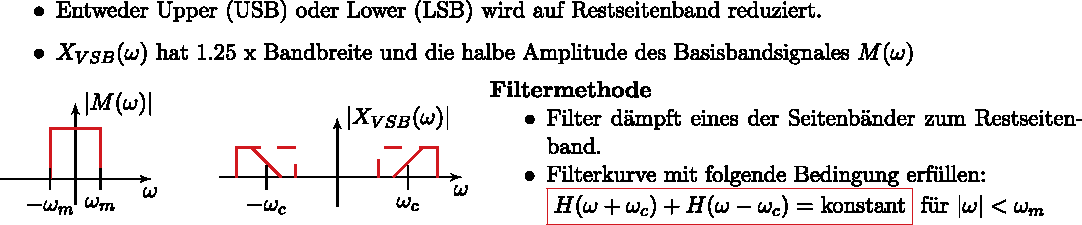
\includegraphics{content/06_amplitudenmodulation/VSB_mod.pdf}
\paragraph{Demodulation}
\textbf{Kohärente Demodulation ist erforderlich!}\\
Demodulation erfolgt gleich wie bei SSB-AM

\subsubsection{Quadraturamplitudenmodulation (QAM) S. 58}
Gleichzeitige Übertragung von zwei Basisbandsignalen im gleichen Frequenzband aber mit zwei orthogonalen Trägersignalen $cos(\omega_c t)$ und $sin(\omega_c t)$.\\
Vorteil: ebenso hohe Bandbreiteneffizienz wie SSB-AM \\
Nachteil: technisch aufwändiger als DSB-AM
\paragraph{Modulation und Demodulation S. 59}
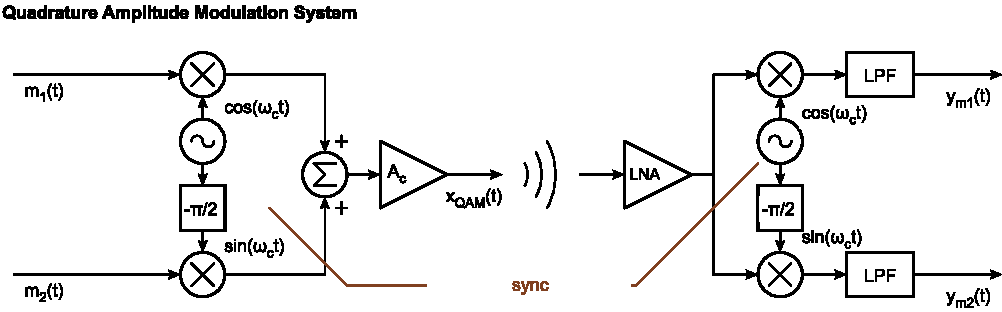
\includegraphics[width=.8\linewidth]{content/06_amplitudenmodulation/abbildung5_25.pdf}\\
\efbox[linecolor=red]{$B_{QAM} = 2\cdot max(B_{m1}, B_{m2}) $} $\rightarrow$ gleich wie DSB; Wenn $m_1$ die Hilberttrafo von $m_2$ ist, dann Bandbreite wie SSB $B_{SSB} = B_m$
\subsection{Winkelmodulation (FM/PM) S. 60}
Besser Störfestigkeit aber grösserer Bandbreitenbedarf als AM.

\begin{minipage}{.45\linewidth}
	Äquivalente Basisbanddarstellung der Grosshubwinkelmodulation
	\newline
	
	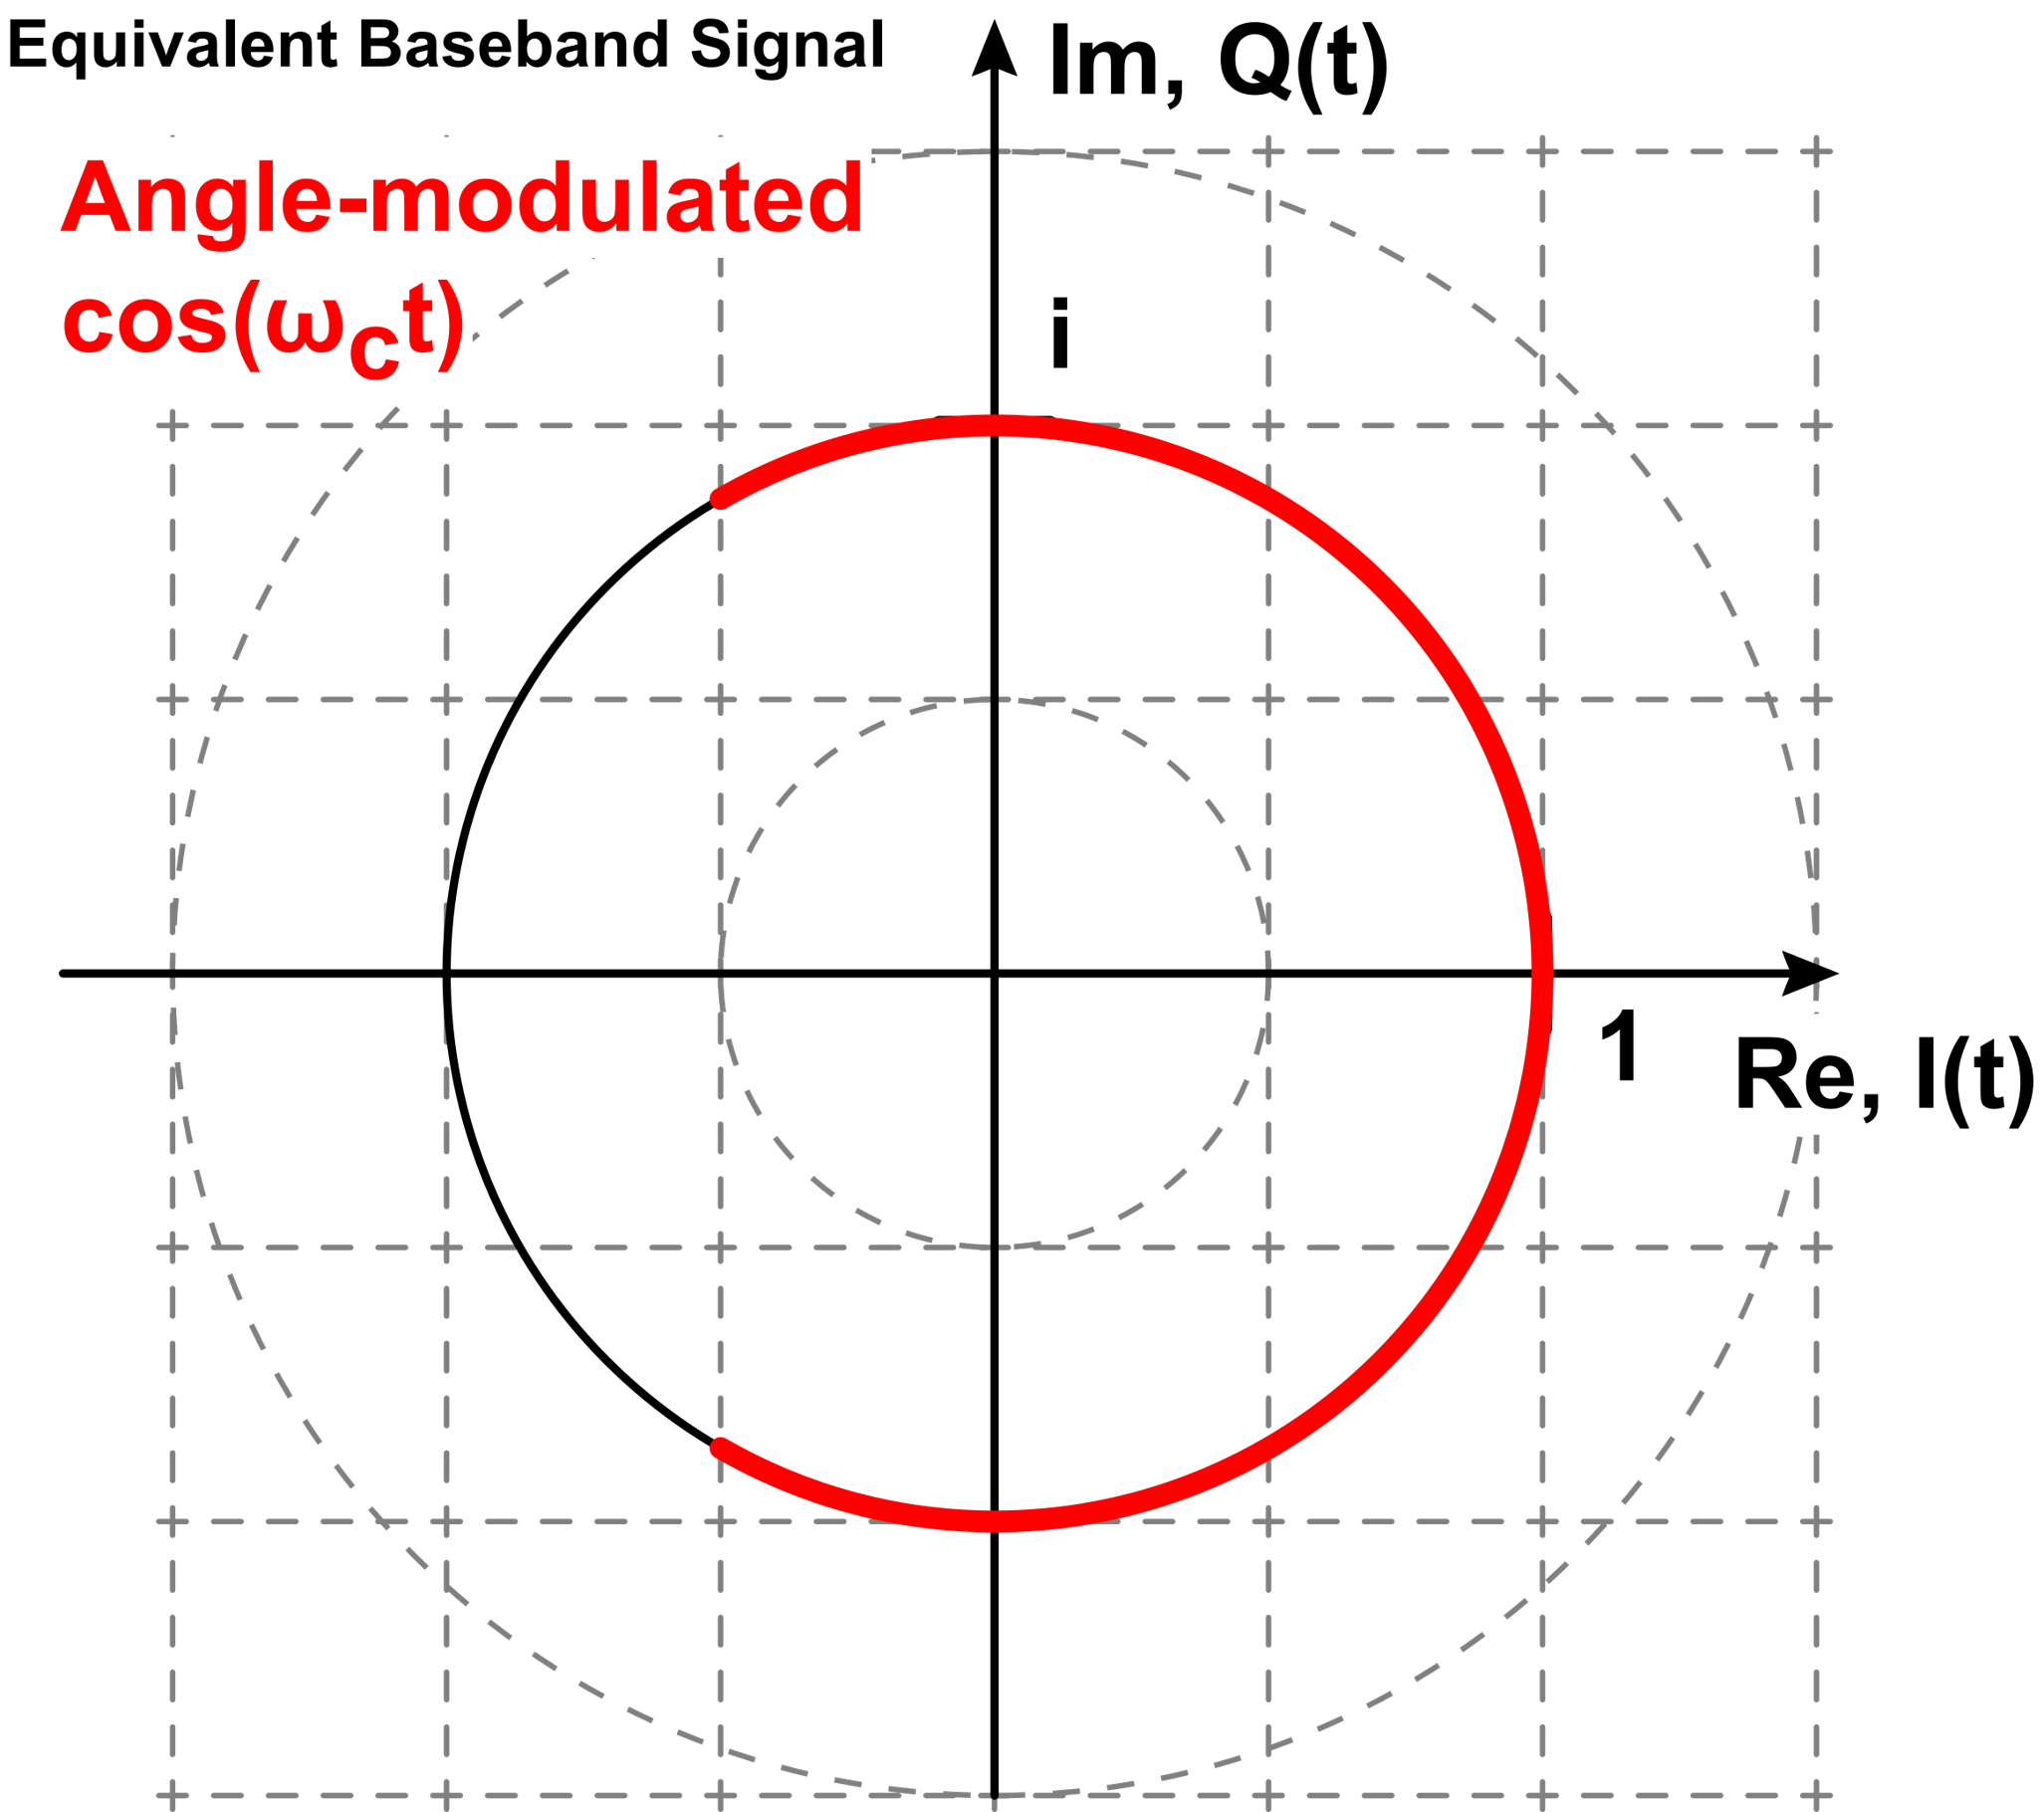
\includegraphics[width=.6\linewidth]{content/06_amplitudenmodulation/PM_zeiger.png}
\end{minipage} \hspace{.1\linewidth}
\begin{minipage}{.45\linewidth}
	
	Zeigerdiagramm des winkelmodulierten Trägersignals
	
	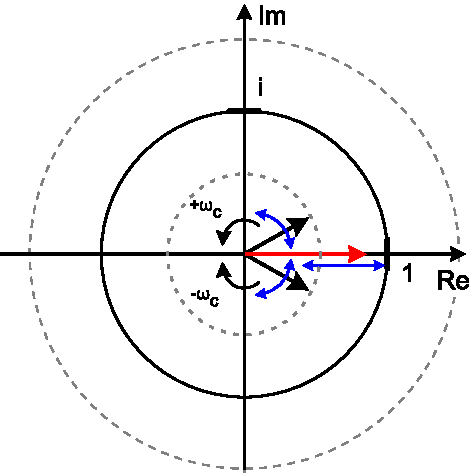
\includegraphics[width=.6\linewidth]{content/06_amplitudenmodulation/abbildung5_26.pdf}
\end{minipage}

\begin{table}[H]
	\begin{tabularx}{\linewidth}{m{.38\linewidth} m{.26\linewidth} m{.3\linewidth}}
		\begin{minipage}{.95\linewidth}
			\textbf{Phasenmodulation PM}\\
			$m(t)$ $\sim$ Phasenabweichung zum Referenzträgersignal\\
			\boxedeq{ \begin{split}
				x_{PM}(t)=A_c\cdot cos(\omega_c t + k_pm(t))\\
				k_p = \text{Phasenhubkonkstante [rad]} \\
				k_p = 2\pi \cdot  \frac{t_{delay,max}}{T_c}
			\end{split}
			}
		\end{minipage}

	&
	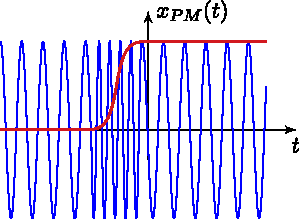
\includegraphics[width=\linewidth]{content/06_amplitudenmodulation/xpm.pdf}
	&
	\begin{minipage}{\linewidth}
		Momentane Phasenabweichung\\
		\efbox[linecolor=red]{$\varphi(t) = k_P \cdot m(t)$}\\
		Momentane Frequenzabweichung \\
		\efbox[linecolor=red]{$ \frac{d\varphi(t)}{dt} = k_P \cdot \frac{dm(t)}{dt}$}\\
		Momentane Frequenz\\
		\efbox[linecolor=red]{$\omega_i(t)=\omega_c+\frac{d\varphi(t)}{dt}$}\\
		Maximale Frequenzabweichung (z.B. bei Jitter)\\
		\efbox[linecolor=red]{$ \Delta \omega = \max( \frac{d\varphi(t)}{dt}) $}
	\end{minipage}
	\\
	\begin{minipage}{.95\linewidth}
		\textbf{Frequenzmodulation FM}\\
		$m(t)$ $\sim$ Frequenzabweichung zum Referenzträgersignal\\
		\boxedeq{\begin{split} x_{PM}(t)=A_c\cdot cos(\omega_c t + k_F\int m(\tau)d\tau)\\
				k_F = \text{Frequenzhubkonkstante [rad/s]} \\
				\frac{A_{k_F} \cdot mpk}{\omega_m} = \varphi_peak(t) \cdot \frac{2\pi}{360} 			
		\end{split}}
	\end{minipage}
	&
	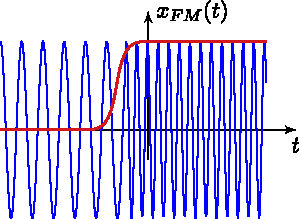
\includegraphics{content/06_amplitudenmodulation/xfm.pdf}
	&
	\begin{minipage}{\linewidth}
		Momentane Phasenabweichung\\
		\efbox[linecolor=red]{$\varphi(t) = k_F \int m(\tau)d\tau$}\\
		Momentane Frequenzabweichung \\
		\efbox[linecolor=red]{$ \frac{d\varphi(t)}{dt} = k_F \cdot m(t)$}\\
		Momentane Frequenz\\
		\efbox[linecolor=red]{$\omega_i(t)=\omega_c+k_F \cdot m(t)$}\
	\end{minipage}
	\end{tabularx}
\end{table}

\subsubsection{Äquivalenz PM und FM}
PM und FM können äquivalent realisiert werden (mit zusätzlichem Integrator oder Differenziator)\\
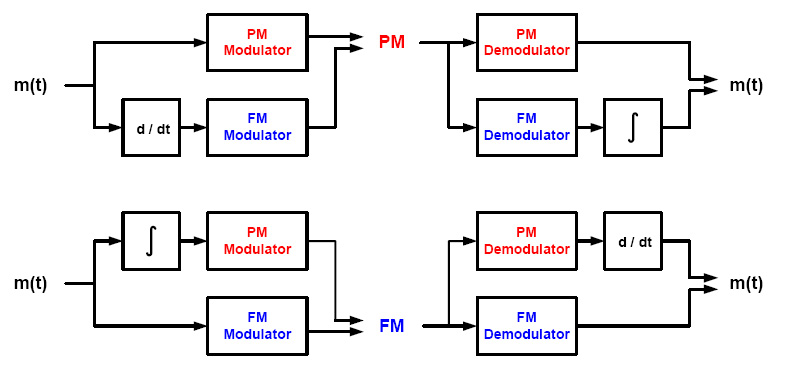
\includegraphics[width=\linewidth]{content/06_amplitudenmodulation/PMundFM.png}

\subsubsection{Spektrum der Winkelmodulation S. 62}
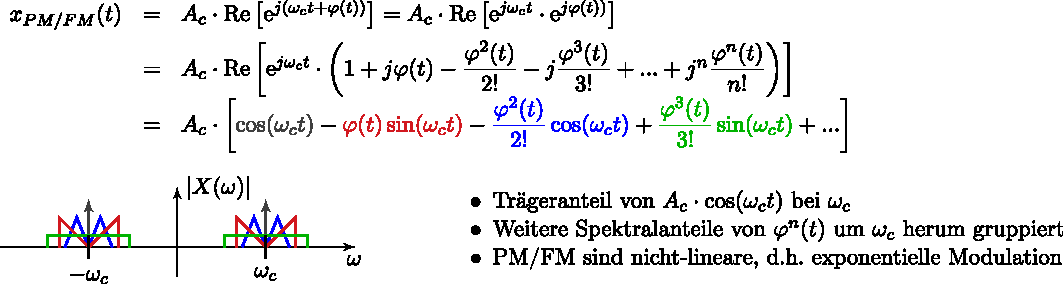
\includegraphics[width=\linewidth]{content/06_amplitudenmodulation/spektrumWinkelmodulation.pdf}

\subsubsection{Kleinhub Winkelmodulation S. 62}
\begin{table}[H]
	\begin{tabularx}{\linewidth}{m{.65\linewidth} m{.35\linewidth}}
		\begin{minipage}{\linewidth}
				Kleinhubmodulation funktioniert in der Praxis bei ca: \efbox[linecolor=red]{$|\varphi(t)| < 0.2 \text{ rad}$} bzw. 10 bis 12 Grad. \\
				Dann gilt: \efbox[linecolor=red]{$x_{NB\phi M}(t) \approx A_c \cdot cos(\omega_c t) - A_c \cdot (\varphi(t)\cdot sin(\omega_ct))$} \\
				\textbf{Demodulation:} mit kohärentem Produktdetektor\\ $\rightarrow x_{NB-PM/FM}(t)\cdot (-sin(\omega_c t))$ \\
				Bild rechts: äquivalente Basisbanddarstellung des Signals\\ $x_{NB-PM}(t) = 0.05 \cdot \sin(2\pi \cdot 200 t) + 1\cdot \sin(2\pi \cdot 1000 t)$\\
				Wobei nur spannend ist, dass die Signalamplitude im Vergleich zur Trägeramplitude sehr klein ist und der Träger eine Sinusschwingung ist (siehe Formeln zu beginn des Kapitels)
		\end{minipage}
		&
		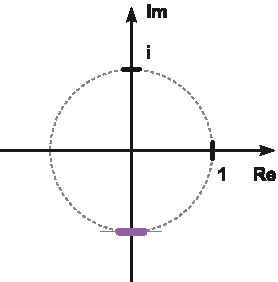
\includegraphics[width=.8\linewidth]{content/06_amplitudenmodulation/eqBase_NBAM.pdf}
	\end{tabularx}
\end{table}

\paragraph{Spektrum S. 62}
\includegraphics[width=.8\linewidth]{content/06_amplitudenmodulation/SpektrumNB_PM.pdf}\\
\textbf{Vergleich AM und NP-PM:} Qualitativ gilt für die Amplitudenspektren $|X_{AM}(\omega)| = |X_{NBPM(\omega)}$

\subsubsection{Grosshub Winkelmodulation S. 63}
WideBand Angle Modulation, siehe auch  Skript Seite 67 \hspace{.3cm} \efbox[linecolor=red]{$|\varphi (t)| > 1$}
	\begin{list}{$\bullet$}{\setlength{\itemsep}{0cm} \setlength{\parsep}{0cm} 	\setlength{\topsep}{0cm}} 
	\item nicht lineare Terme von $\varphi (t)$ nicht mehr vernachlässigbar
	\item analytische Bestimmung des Spektrums nur noch für Eintonsignale durchführbar
	\item Überlagerungssatz nicht mehr gültig
	\item $x_{FM/PM}$ ist zu $m(t)$ stark nicht linear
	\item im Frequenzspektrum treten $\sim m(t)$ Anteile auf
\end{list}
\begin{table}[H]
	\begin{tabularx}{\linewidth}{m{.7\linewidth} m{.3\linewidth}}
		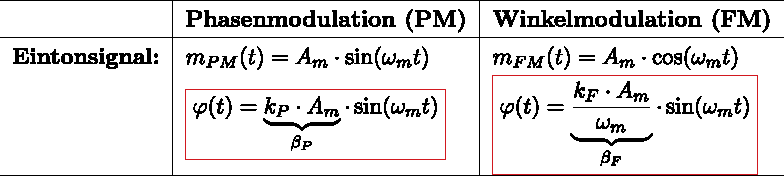
\includegraphics{content/06_amplitudenmodulation/WB_PM.pdf}
		&
		\begin{minipage}{.9\linewidth}
			\begin{center}
				Modulationsindex:\\
				\efbox[linecolor=red]{$\beta = \frac{\Delta \omega}{\omega_m}$}\\
				Ist nur für Eintonsignale Definiert!\\
				\efbox[linecolor=red]{$\Delta T=\frac{1}{f_c}\cdot \frac{\beta}{2\pi}$} \\
				"Periodendauer mal normalisierten Winkel"
			\end{center}			
		\end{minipage}
	\end{tabularx}
\end{table}

\subsubsection{Spektrum Einton-Winkelmodulation S. 64}
\vspace{.1cm}
\efbox[linecolor=red]{$x_{ST} = A_c \cdot \Re (e^{j(\omega_c t + \varphi (t))}) = A_c \cdot cos(\omega_c t + \beta \cdot sin(\omega_mt)) = A_c \cdot \sum_{n=-\infty}^{\infty}J_n(\beta) \cdot cos((\omega_c + n\cdot \omega_m)t)$} \\
mit $\varphi(t)$ als Nachrichtensignal gemäss Phasen- oder Winkelmodulation (siehe Tabelle oben) und \\$J_n(\beta)$: Bessel Funktion erster Art und n-ter Ordnung

\begin{minipage}{.7\linewidth}
	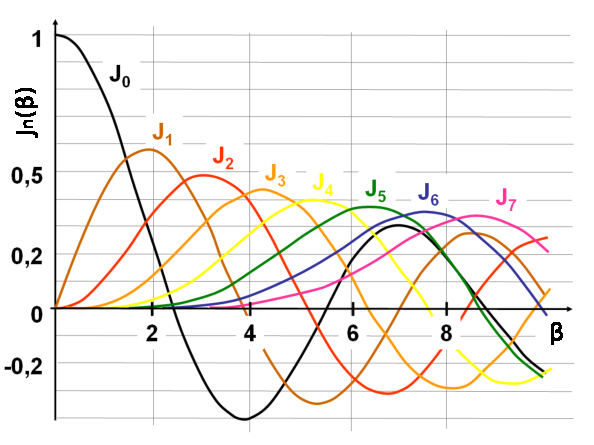
\includegraphics{content/06_amplitudenmodulation/besselfunktionen.pdf}
\end{minipage}
\begin{minipage}{.3\linewidth}
	\textbf{Eigenschaften:}\\
	
	\efbox[linecolor=red]{$J_{-n}(\beta) = (-1)^n\cdot J_n(\beta)$} \\
	
	\efbox[linecolor=red]{$J_{n-1}(\beta) + J_{n+1}(\beta) = \frac{2n}{\beta} \cdot J_n(\beta)$} \\
	
	\efbox[linecolor=red]{$ \sum_{n=-\infty}^{\infty} J^2_n (\beta) = 1$} \\
	
	\efbox[linecolor=red]{$ \beta_n = \Delta T \cdot 2\pi \cdot n \cdot f_c $} \\
	
	$\Delta T$: Zeitverzögerung bezogen auf Grundschwingung ($f_c$) \\
	$n$: n-te Harmonische \\
	
	Tabelle Skript S. 66 bzw. 258 ff.
\end{minipage}

\subsubsection{Bandbreite Einton-Winkelmodulation S. 67}
Theoretisch unendliche Bandbreite \\
Praktisch approximation nach Carson: \efbox[linecolor=red]{$B_{ST} = 2 \cdot (\Delta f+f_m) = 2 \cdot (\beta + 1) \cdot \frac{\omega_m}{2\pi}$} (min. \qty{98}{\%} der Signalleistung)\\
\includegraphics{content/06_amplitudenmodulation/bandbreite.pdf}

\subsubsection[Bandbreite für beliebige m(t)]{Bandbreite für beliebige $m(t)$ S. 67}
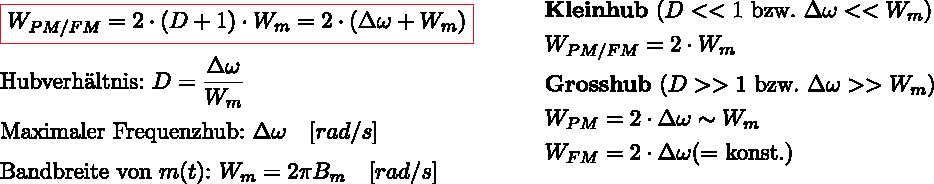
\includegraphics{content/06_amplitudenmodulation/bandbreiteBeliebigem.pdf}

\subsubsection{Realisierung}
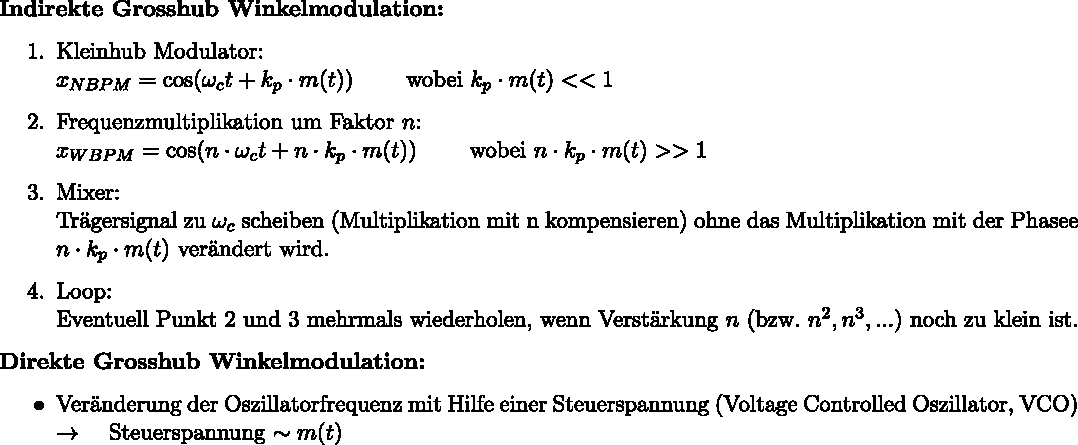
\includegraphics{content/06_amplitudenmodulation/realisierungGrosshubWinkelmod.pdf}

\subsubsection{Demodulation}
\paragraph{Phase Locked Loop (PLL)}
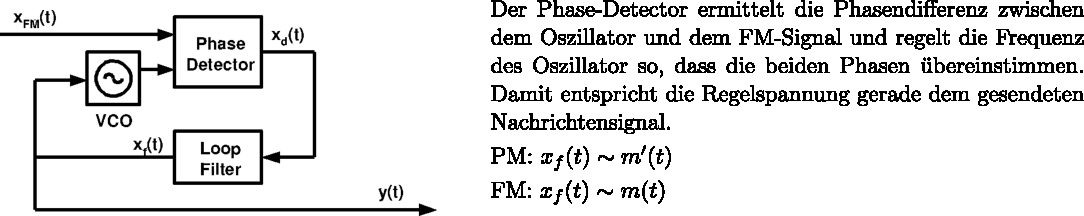
\includegraphics{content/06_amplitudenmodulation/PLLdemod.pdf}

\paragraph{Frequenz-Diskriminator}
Die Amplitude des Ausgangssignals eines Frequenz-Diskriminators ist proportional zur Momentanfrequenz des Eingangssignals. $\rightarrow y_d(t) = k_d \cdot \varphi'(t)$ \\
\textbf{PM:} $y_d(t)=k_d\cdot k_p \cdot m'(t)$ \\
\textbf{FM:} $y_d(t) = k_d \cdot k_f \cdot m(t)$

\subsubsection{FM Empfänger S. 68}
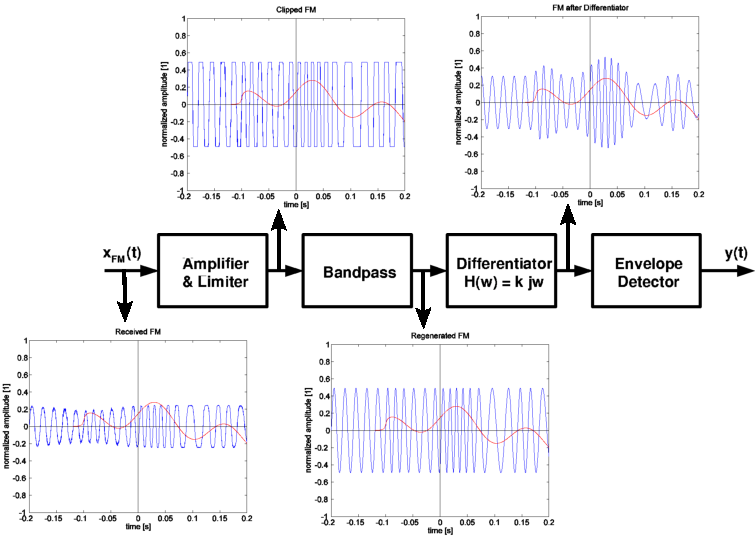
\includegraphics{content/06_amplitudenmodulation/FMreceiver.pdf}
\newpage
	\section{Digitalisierung von Signalen S. 71}
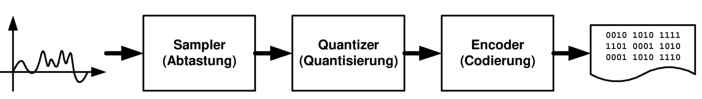
\includegraphics{content/07_digsig/digitalisierungBlockschema.pdf}
\begin{table}[H]
	\begin{tabularx}{\linewidth}{X|X}
		\begin{list}{$\bullet$}{\setlength{\itemsep}{0cm} \setlength{\parsep}{0cm}
				\setlength{\topsep}{0cm}} 
				\item Zeitdikretisierung, endliche Anzahl von Werten pro Zeit
				\item störungsfreie Übertragung
				\item Codierung (z.B. Fehlerkorrektur oder Verschlüsselung)
		\end{list}
	&
		\begin{list}{$\bullet$}{\setlength{\itemsep}{0cm} \setlength{\parsep}{0cm}
		\setlength{\topsep}{0cm}} 
			\item Quantisierung, endliche Anzahl an Amplitudenwerten (Bits)
			\item neue möglichkeiten für Signalverarbeitung
			\item Speicherung auf einheitlichen Medien
	\end{list}
	\end{tabularx}
\end{table}

\subsection{Abtastung S. 73}
\subsubsection{Ideale Abtastung S.75}
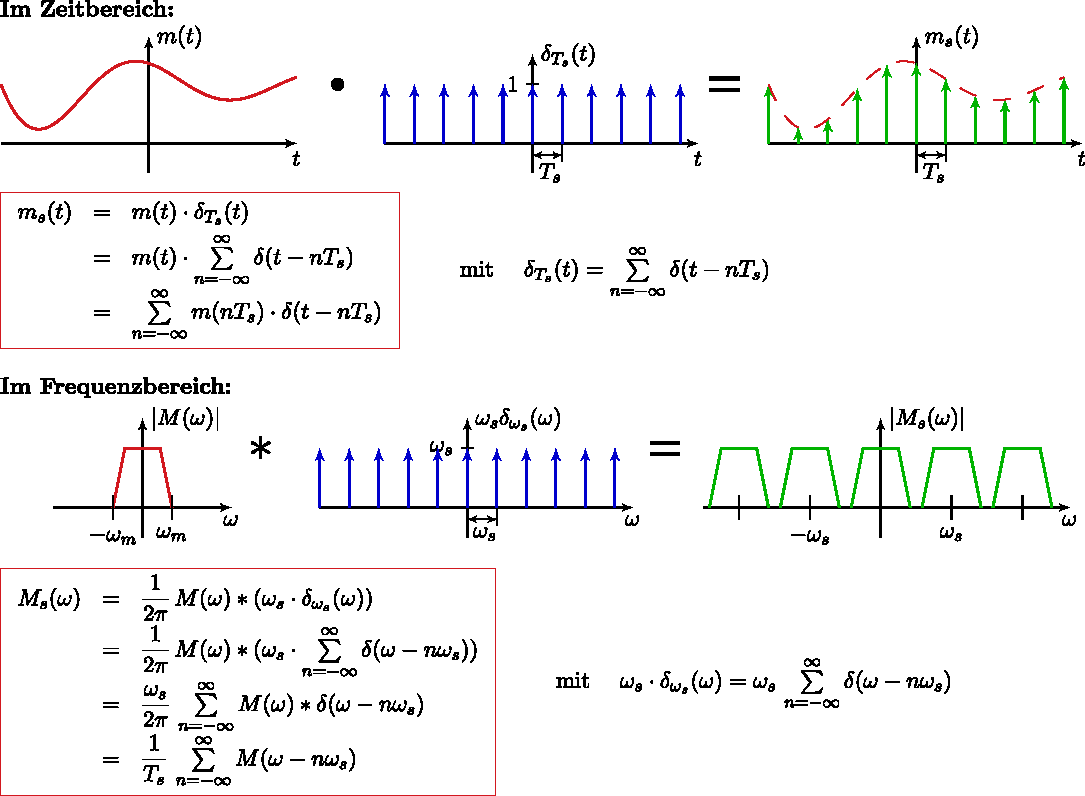
\includegraphics[width=.90\linewidth]{content/07_digsig/idealeAbtastung.pdf}

\subsubsection{Rekonstruktion mit Tiefpass S. 78}
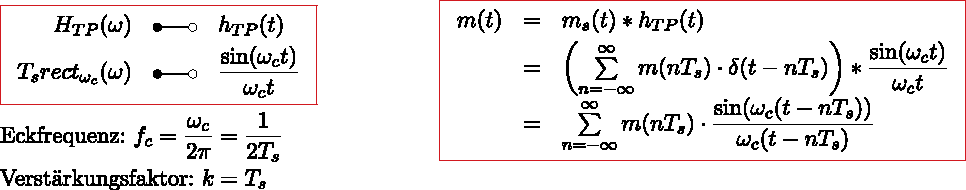
\includegraphics[width=.95\linewidth]{content/07_digsig/rekonstruktionTP.pdf}

\subsubsection{Natural Sampling S. 73}
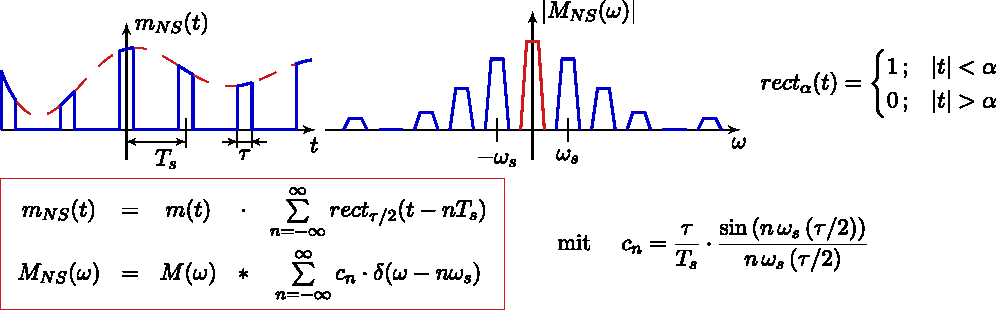
\includegraphics{content/07_digsig/naturalSampling.pdf}\\
\textbf{Rekonstruktion:} Bei der Rekonstruktion muss das Signal nach dem Tiefpass noch mit dem Faktor $\frac{T_s}{\tau}$ multipliziert werden, um die Dämpfung wieder aufzuheben.

\subsubsection{Sample {\&} Hold (ZOH), Flat-Top Sampling S. 78}
ZOH $\rightarrow$ Zero Order Hold. $H_{ZOH}(\omega) = \tau \cdot \frac{sin(\frac{\tau \omega}{2})}{\frac{\tau \omega}{2 }} \;\;\; , \;\;\; \tau \leq T_s$\\
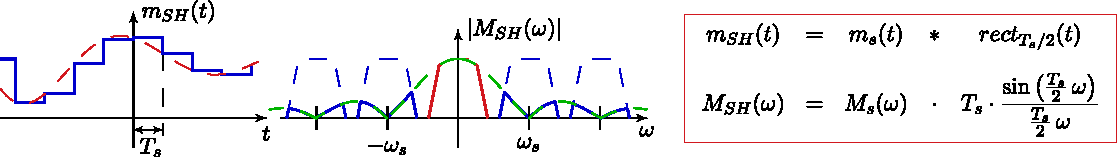
\includegraphics{content/07_digsig/flattopsampling.pdf}

\subsubsection{Nyquist-Shannon Abtasttheorem S. 76}
	\begin{list}{$\bullet$}{\setlength{\itemsep}{0cm} \setlength{\parsep}{0cm}
	\setlength{\topsep}{0cm}} 
		\item Nachrichtensignal muss auf eine Bandbreite begrenzt sein $|M(\omega)|\approx 0 \text{ für } \omega > 2\pi B_m$ (Aliasing S. 77)
		\item im Basisband darf es keine Überlappungen von Teilspektren geben, d.h. $f_s$ muss die Spektralanteile genügend weit vom ursprünglichen Spektrum wegschieben.
	\end{list}

\begin{minipage}{.3\linewidth}
	\textbf{Abtasttheorem für Basisbandsignale:} \efbox[linecolor=red]{$f_s > 2 \cdot B_m$}
\end{minipage}
\begin{minipage}{.7\linewidth}
	\begin{table}[H]
		\begin{tabularx}{\linewidth}{|m{.4\linewidth} m{.6\linewidth}}
			Nyquistrate: $f_{sN} = 2B_m$	&	Samplingfrequenz: $[f_s] = Hz$	\\
			Nyquistfrequenz: $f_N = \frac{f_s}{2}$	&	Nachrichtenfrequenz: $[f_m] = Hz$ \\
			Nyquistintervall: $T_N = \frac{1}{2B_m}$	&	Nachrichtenbandbreite: $[B_m] = Hz$\\
		\end{tabularx}
	\end{table}
\end{minipage}

\paragraph{Abtasttheroem für Bandpasssignale S. 76 (Subsampling)}
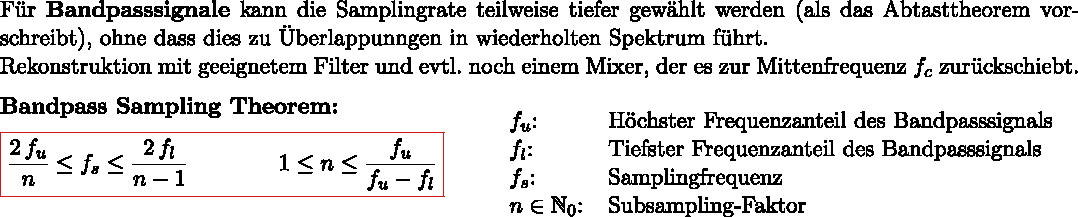
\includegraphics{content/07_digsig/subsampling.pdf}
\newpage
\paragraph{Interpolation im digitalen Bereich S. 80 (Oversampling)}
Bei Oversampling werden auf \textbf{digitaler Seite Zwischenwerte berechnet} (Interpolation) um mehr Samples zu generieren vor der D/A Wandlung. Das führt dazu, dass das \textbf{Basisband erweitert} wird (also die Blöcke im Amplitudendichtespektrum auseinandergeschoben werden, vgl Abbildung unten und "ideale Abtastung").\\
\vspace{.3cm}
Berechnung der Zwischenwerte: \efbox[linecolor=red]{$m(t)=\sum_{n=-\infty}^{\infty} m(nT_0) \frac{sin(\omega_c(t-nT_0))}{\omega_c(t-T_0)} \text{  mit  } \omega_c = \frac{\omega_s}{2}$}\\
\textbf{Vorteile:} TP-Filter kann einfacher realisiert werden (\textbf{weniger Steilheit} erforderlich), Signal wird originalgetreuer rekonstruiert; Amplitudengang des ZOH kann digital kompensiert werden.

\begin{center}
	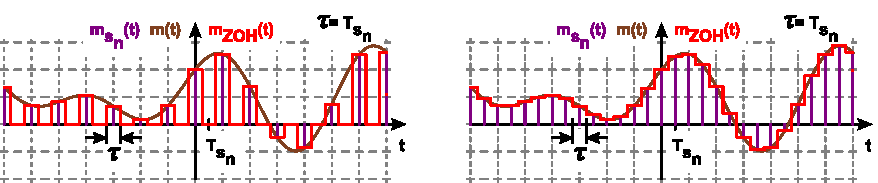
\includegraphics[width=.75\linewidth]{content/07_digsig/abbildung6_6.pdf}\\
	Zweifach interpoliertes Zero-Order Hold Signal, vor und nach dem digitalen Tiefpassfilter\\
	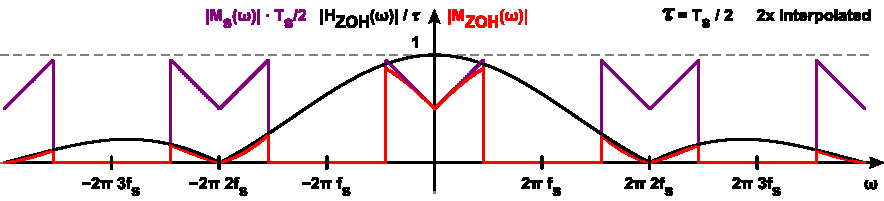
\includegraphics[width=.75\linewidth]{content/07_digsig/abbildung6_7.pdf}\\
	Zweifach interpoliertes Zero-Order Hold Signal im Frequenzbereich
\end{center}

\subsection{Quantisierung S. 81}
Nach dem Sampling liegen die zeitdiskreten Abtastwerte noch immer \textbf{amplitudenkontinuierlich} vor!
\subsubsection{Gleichförmige Quantisierung S.82}

\begin{tabularx}{\linewidth}{p{.25\linewidth} p{.2\linewidth} p{.25\linewidth} p{.2\linewidth}}
	Skalierung von $m(t)$:    & $|m_n(t) < 1$ & Wortlänge der Samples: & n Bits \\
	Quantisierungsintervalle: & $L = 2^n$     & Intervallbreite:       & $\Delta = 2/L = 2^{-(n-1)}$
\end{tabularx}\\

\paragraph{Quantisierungsrauschen}
\begin{tabularx}{\linewidth}{p{.3\textwidth} p{.65\textwidth}}
	Fehlersignal $q_e(nT)$:	& Abweichung vom effektiven Wert zum quantisierten Wert. Char. von weissem Rauschen $->$ gleichverteilt im Intervall $-\Delta/2 ... \Delta/2$\\
	Maximaler Fehler:		&  $-\Delta/2 < q_e(nT_s) < \Delta/2$ \hspace{2cm} \efbox[linecolor=red]{$P_{qe}=N=\frac{1}{\Delta} \int_{-\Delta/2}^{\Delta/2} q_e^2dq_e = \frac{\Delta^2}{12}$}
\end{tabularx}\\

\paragraph{SNR Signal-Rausch Verhältnis S. 82}
\begin{tabularx}{\linewidth}{p{.45\linewidth} p{.5\linewidth}}
	\begin{minipage}{\linewidth}
			\begin{list}{$\bullet$}{\setlength{\itemsep}{0cm} \setlength{\parsep}{0cm}
				\setlength{\topsep}{0cm}} 
			\item Signal wird maximal ausgesteuert mit\\ $|m(t)|_max = 1$
			\item $|m(t)|$ ist über Intervall $[-1...1]$ gleichverteilt
		\end{list}
	\end{minipage}
&
\begin{minipage}{\linewidth}
	\boxedeq{\begin{split} SNR_q=\frac{S}{N_q}=\frac{m^2_{RMS}}{\frac{\Delta^2}{12}} = \frac{P_m}{P_{qe}}= \frac{(\frac{1}{C})^2}{\frac{(\frac{1}{2^{n-1}})^2}{12}} = \frac{3}{C^2} \cdot 2^{2n} \\
	SNR_{q,dB} = n \cdot \qty{6.02}{\dB} + 10 \cdot log_{10} (\frac{3}{C^2}) \qty{ }{\dB} \end{split}}
\end{minipage}
\end{tabularx}

\subsubsection{Ungleichförmige Quantisierung S. 83}
	\begin{list}{$\bullet$}{\setlength{\itemsep}{0cm} \setlength{\parsep}{0cm}
		\setlength{\topsep}{0cm}} 
		\item Bei gleichförmiger Quantisierung ist N konstant $\rightarrow$ Verschlechterung der SNR bei tiefen Signalpegeln
		\item bei \textbf{Sprachsignalen vorwiegend kleine Pegel} (nicht gleichverteilt!)
		\item Quanatisierungsintervalle $\Delta$ sind für kleine Signalpegel klein und für grosse Signalpegel grösser $\rightarrow$ SNR wird verbessert
	\end{list}

\subsection{Deltamodulator S. 88}
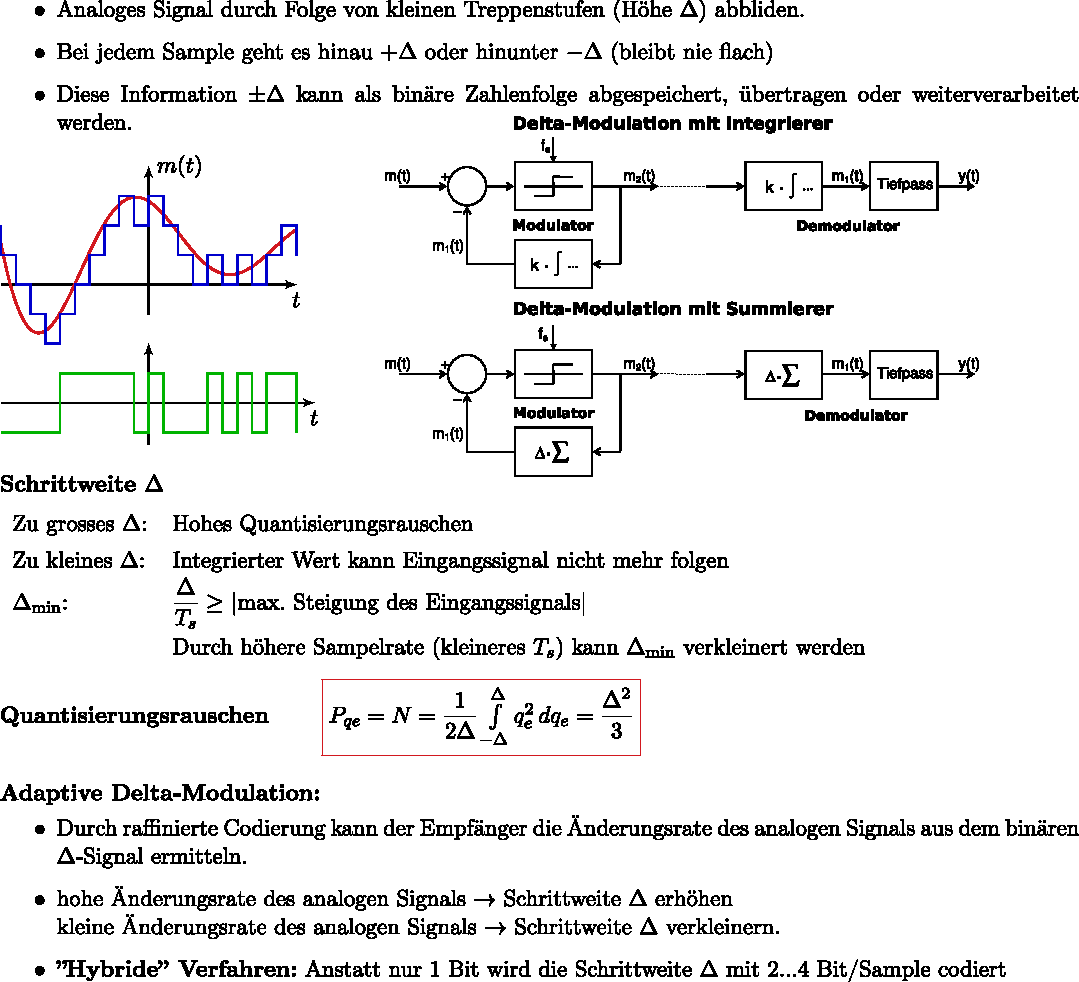
\includegraphics[width=.95\linewidth]{content/07_digsig/deltamodulator.pdf}\\
\subsection{Delta-Sigma Modulator S. 89}
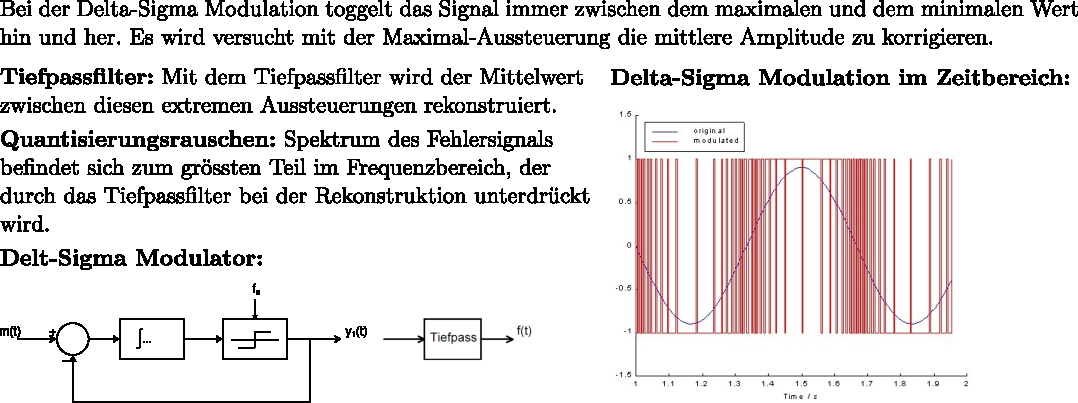
\includegraphics[width=.95\linewidth]{content/07_digsig/deltasigmamodulator.pdf}\\

	\section{Übertragung von digitalen Signalen S. 93}
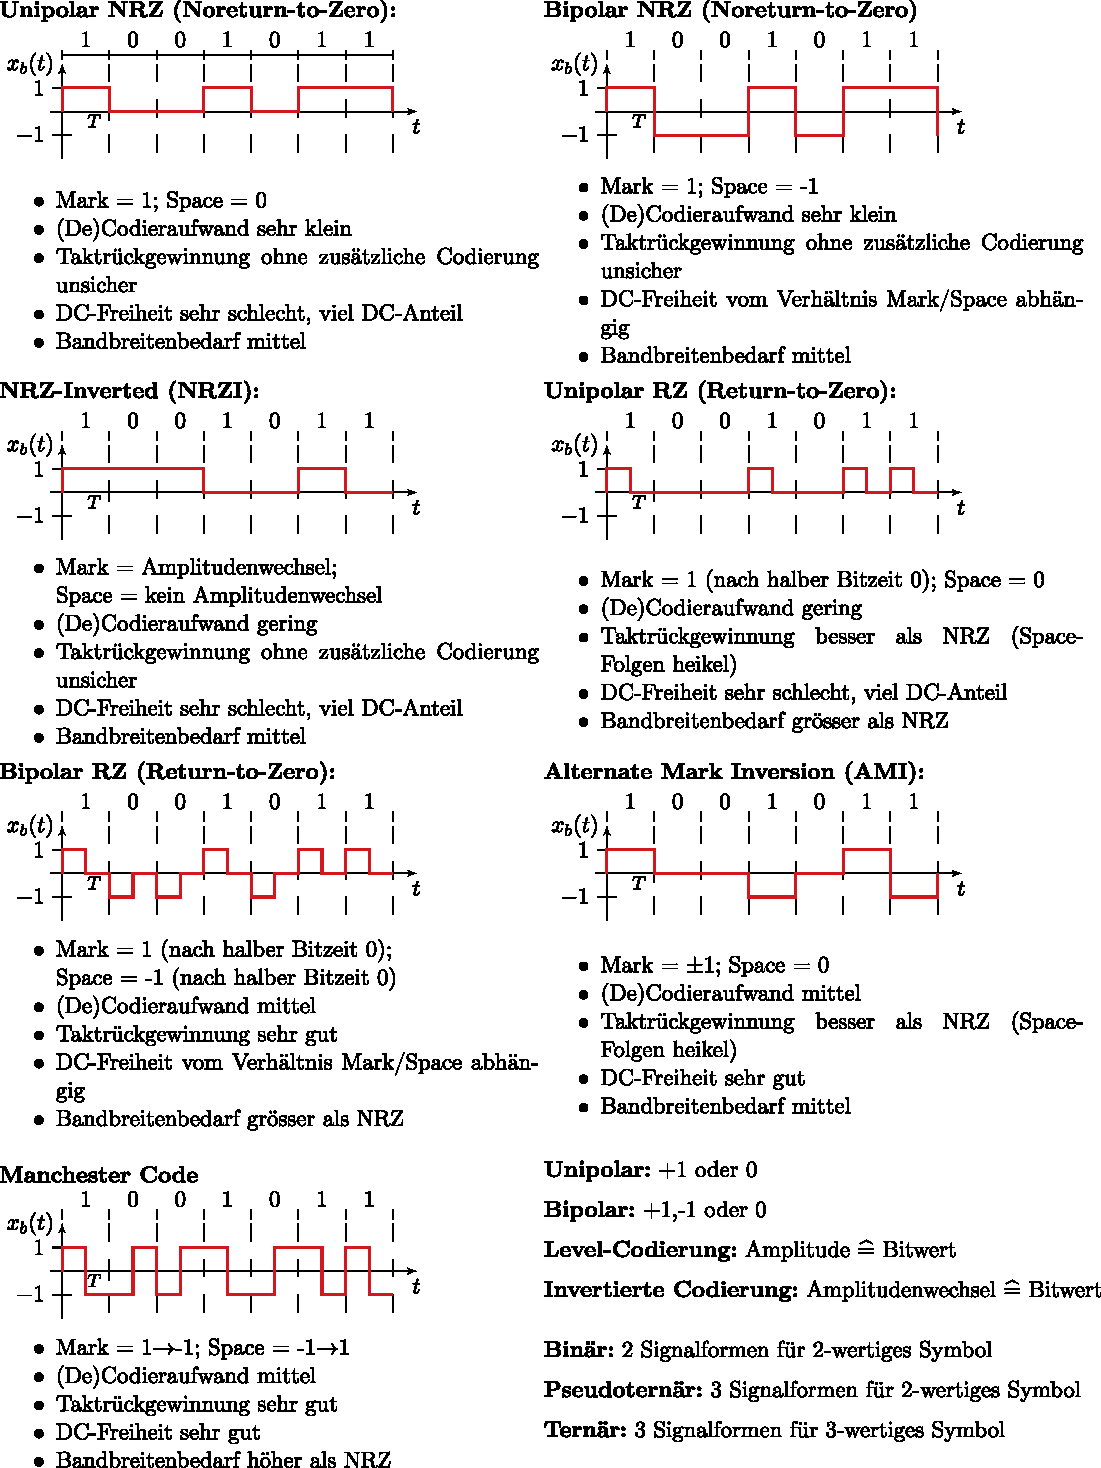
\includegraphics{content/08_digsigtransmit/leitungscodierung.pdf}\\
	\newpage
\begin{tabularx}{\linewidth}{p{.1\linewidth} p{.4\linewidth} p{.1\linewidth} p{.4\linewidth}}
	NRZ: & ZOH über ganze Symbolzeit & Mark: & übertragenes Bit mit Wert 1 \\
	RZ: & ZOH nur über halbe  Symbolzeit & Space: & übertragenes Bit mit Wert 0 \\
	 & Scrambler S. 96, Bitstopfen (bit stuffing) S.  &96 & 8b10b Codierung S. 97
\end{tabularx}

\subsection{Bandbreitenbedarf von PCM (Pulse-Code-Modulation) S. 104}

Bandbreitenbedarf ist nicht explizit berechenbar, er ist abhängig von Anzahl Bits pro Symbolzeit und\\ Leitungscodierungsart.

\subsubsection{min. Bandbreitenbedarf im Binären Fall S.105}
\begin{tabularx}{.6\linewidth}{m{.4\linewidth} m{.3\linewidth} m{.3\linewidth}}
	Samplingrate: 			& $f_s > 2\cdot B_m$ 	&
	\multirow{4}{.75\linewidth}{\begin{minipage}{\linewidth}
		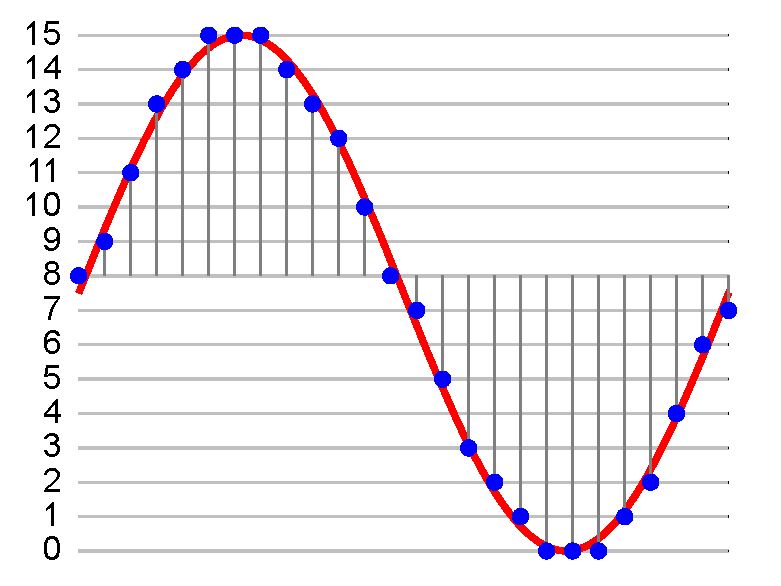
\includegraphics[width=\linewidth]{content/08_digsigtransmit/pcm.pdf}\\
		4 Bit PCM 
	\end{minipage}} \\
	Bitrate: 				& $n\cdot f_s > 2n \cdot B_m$ \\
	minimale Bandbreite:	& \efbox[linecolor=red]{$B_{PCM} = \frac{1}{2} \cdot n \cdot f_s > n\cdot B_m$} \\
	effektiver Bandbreitebedarf: (weil es keine idealen Filter gibt) & \efbox[linecolor=red]{$B_{eff} > B_{PCM} > n \cdot B_{m}$}
\end{tabularx}

\subsection{Pulsformfilter S. 106}
\subsubsection{Intersymbol Interferenz (ISI)}
	\begin{list}{$\bullet$}{\setlength{\itemsep}{0cm} \setlength{\parsep}{0cm} \setlength{\topsep}{0cm}} 
	\item Wenn digitale Signale mit Rechteckimpulsen dargestellt werden, müssen die Pulse verbreitert werden um Bandbreite zu sparen.
	\item Interferenz + weitere Störungen = Bitfehler beim Empfänger
	\item Verarbeitung führt zu Überlappung benachbarter Pulse $\rightarrow$ Intersymbol Interferenz
	\item Bereich für korrekte Entscheidungsschwelle wird verkleinert (vertikale Augenöffnung)
\end{list}
\textbf{Massnahmen gegen Intersymbol Interferenz}: Abtastzeitpunkt muss vom Empfänger optimal gewählt werden (horizontale Augenöffnung). Sendepulse so wählen, dass sich das Auge maximal öffnet (zum Abtastzeitpkt soll keine Interferenz von Nachbarsymbolen vorhanden sein). Synchronisation Sender und Empfänger.
\subsubsection{Erstes Nyquist-Kriterium S. 106}
Wenn erstes Nyquist-Kriterium erfüllt ist, kann Intersymbol-Interferenz eliminiert werden.\\
\begin{tabularx}{\linewidth}{X X}
	\begin{minipage}{\linewidth}
		\textbf{Im Zeitbereich}\\
		\boxedeq{\begin{split} \sum_{n=-\infty}^{\infty} s_p(n\cdot T) \cdot \delta(t-n\cdot T) = s_{p0} \cdot \delta(t) \end{split}} \\
		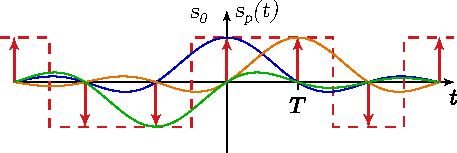
\includegraphics{content/08_digsigtransmit/1nyquisttimedomain.pdf}\\
		Signal muss mit $f_s = \frac{1}{T_s} = \frac{1}{T}$ abgetastet werden. 
	\end{minipage}
	&
	\begin{minipage}{\linewidth}
		\textbf{Im Frequenzbereich}\\
		\boxedeq{\begin{split} \frac{1}{T} \sum_{n=-\infty}^{\infty} S_p(\omega - n\cdot \frac{2\pi}{T}) \cdot \delta(t-n\cdot T) = s_{p0} \end{split}}\\
		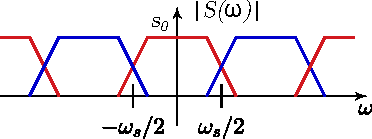
\includegraphics{content/08_digsigtransmit/1nyquistfrequencydomain.pdf}\\
		Das Spektrum muss summiert konstant sein!\\
		Minimale Bandbreite: $B_{min} = \frac{1}{T} = \frac{f_s}{2}$
	\end{minipage}
\end{tabularx}
\subsubsection{Zweites Nyquist-Kriterium S. 111}
Das Augendiagramm soll nicht nur bezüglich der Amplitude, sondern auch bezüglich deR Zeitachse maximal geöffnet sein.\\
Zusätzlich zu den Nullstellen bei $nT$ muss die Impulsform $s_p(t)$ auch Nullstellen haben bei:\\
$\pm \frac{3}{2}T; \pm \frac{5}{2}T; \pm \frac{7}{2}T; ...$\\
Von der Gruppe der Raised-Cosine Pulsen erfüllen nur diejenigen mit Roll-off Faktor $\alpha = 1$ das zweite Nyquist-Kriterium.

\subsubsection{Raised Cosine Pulse S. 107}
\begin{tabularx}{\linewidth}{m{.5\linewidth} m{.5\linewidth}}
	\boxedeq{\begin{split} s_{rc} = \frac{\sin\frac{\pi}{T}t}{\frac{\pi}{T}t} \cdot \frac{\cos\alpha \frac{\pi}{T}t}{1-(2\alpha \frac{\pi}{T}t /\pi)^2} \end{split}}
	&
	Roll-off Faktor $\alpha$ : $0 \geq \alpha \geq 1$
\end{tabularx}

\begin{tabularx}{\linewidth}{m{.65\linewidth} m{.35\linewidth}}
	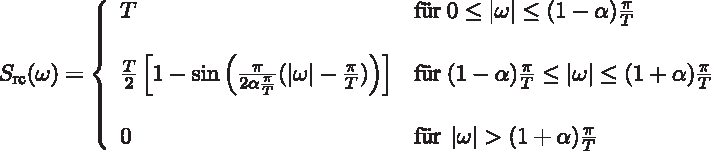
\includegraphics{content/08_digsigtransmit/fancyRCequation.pdf}
	&
	\textbf{Bandbreite:} $B=\frac{f_s}{2} \cdot (1+\alpha) $
\end{tabularx}

\begin{tabularx}{\linewidth}{m{.31\linewidth} m{.36\linewidth} m{.24\linewidth}}
	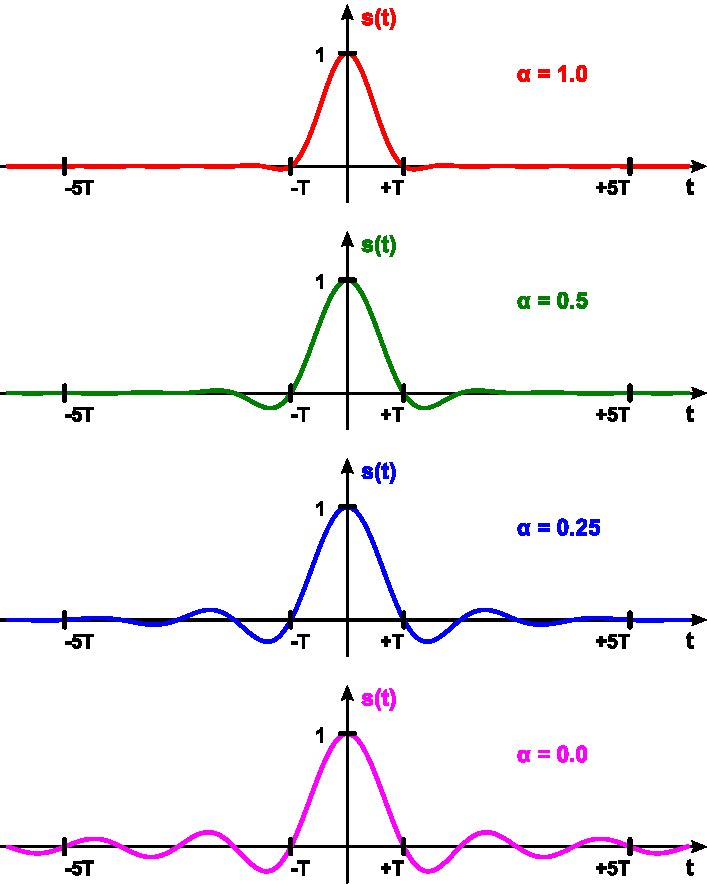
\includegraphics[width=\linewidth]{content/08_digsigtransmit/abbildung7_11.pdf}
	&
	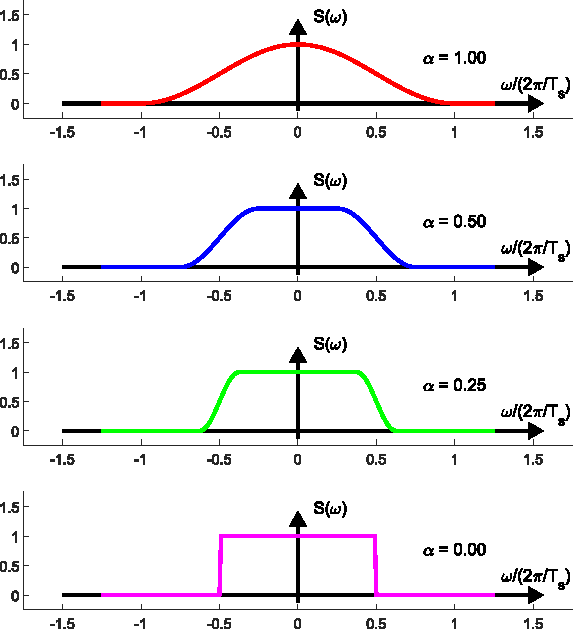
\includegraphics[width=\linewidth]{content/08_digsigtransmit/abbildung7_12.pdf}
	&
	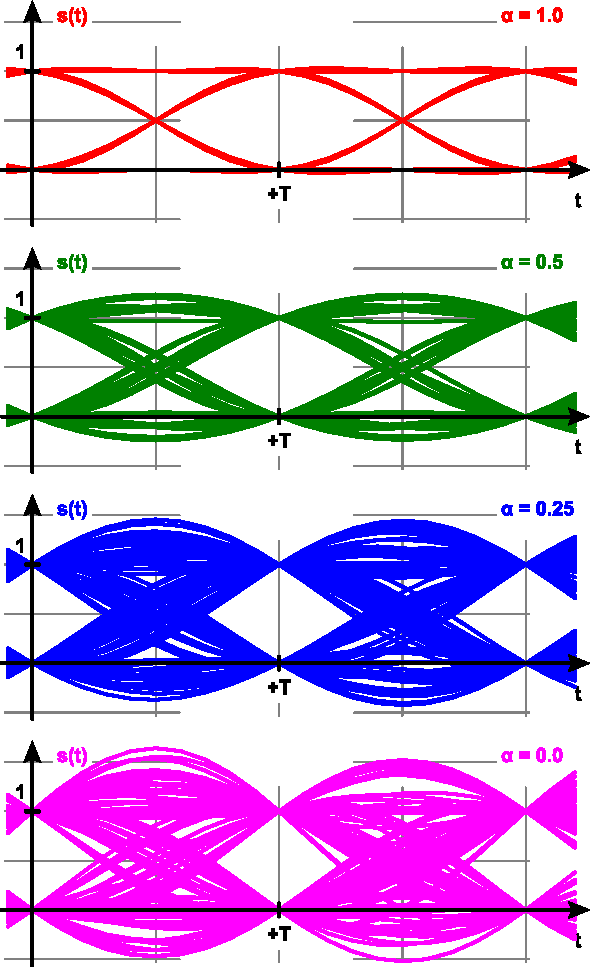
\includegraphics[width=\linewidth]{content/08_digsigtransmit/abbildung7_13.pdf}
\end{tabularx}

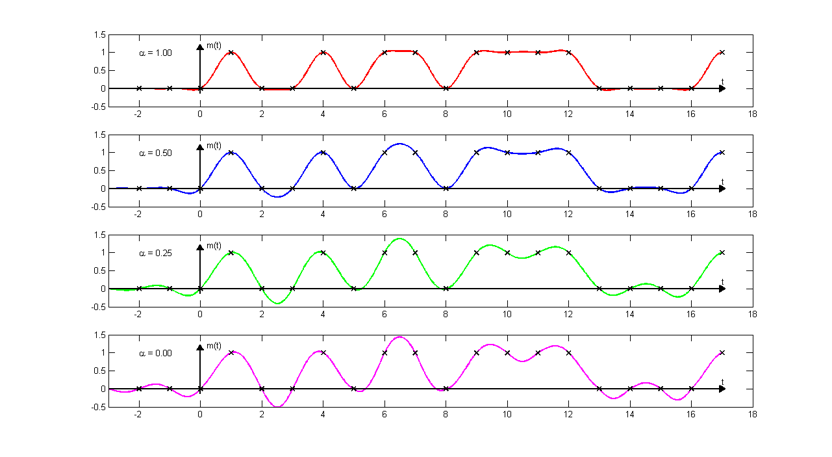
\includegraphics[trim=2cm 1cm 2cm 0cm,clip]{content/08_digsigtransmit/RC_mt_timedomain.png}

\subsection{Digitale Modulation von Trägersignal S. 111}
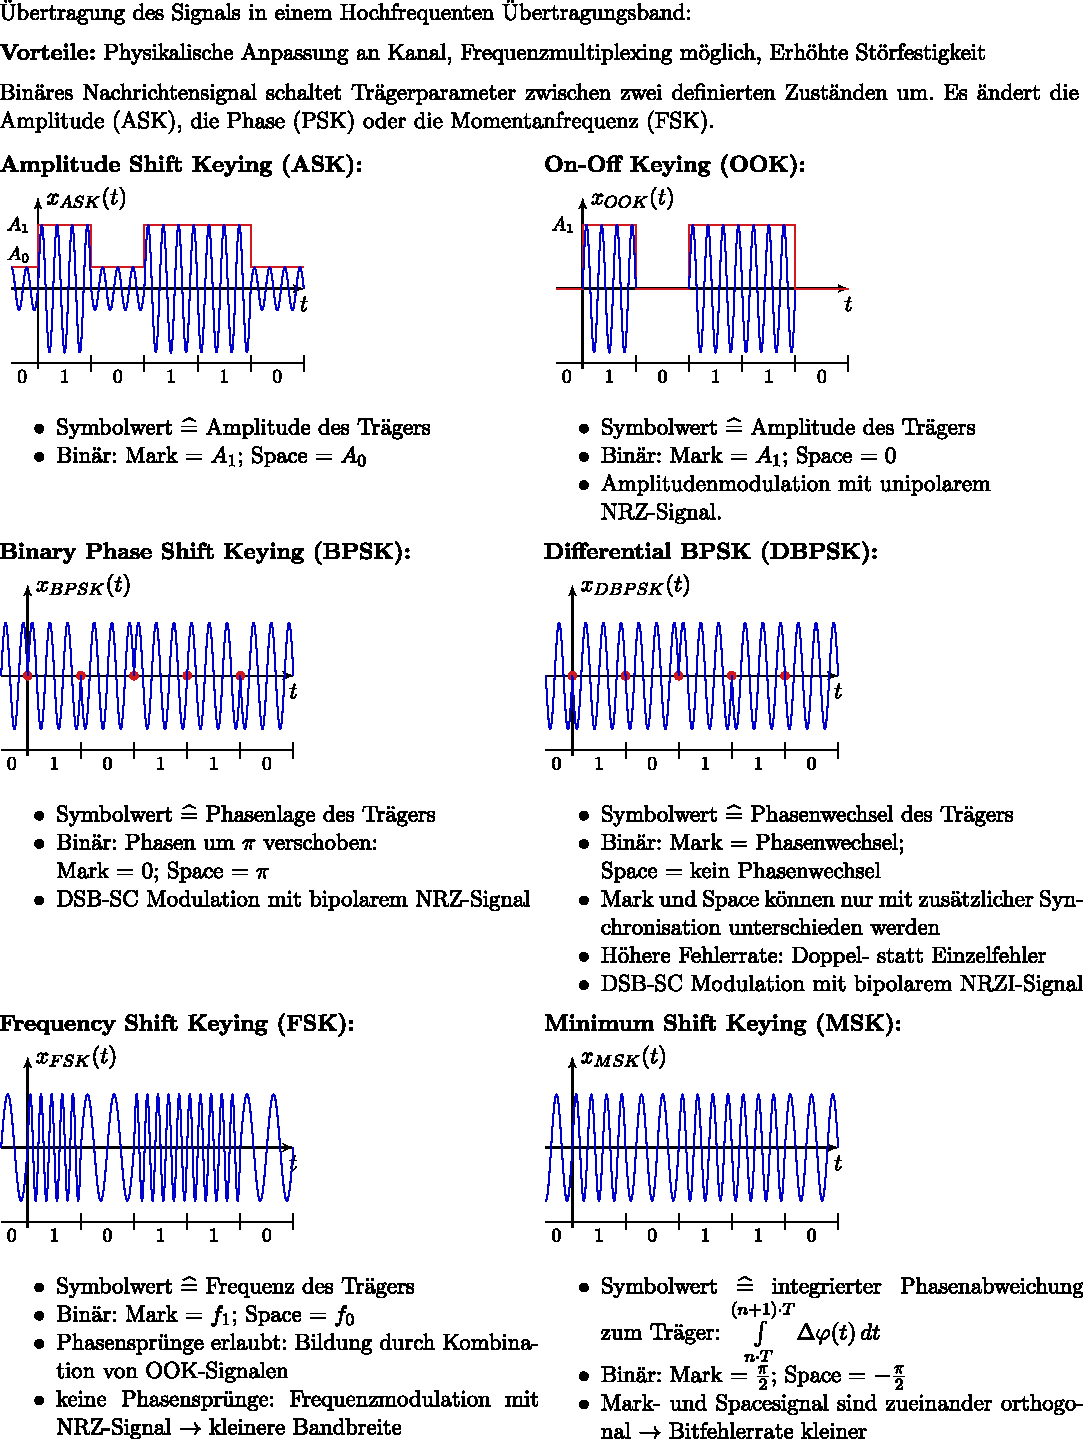
\includegraphics{content/08_digsigtransmit/digModCarrier.pdf}

\subsection{Äquivalente Basisbanddarstellung von Bandpassignalen S. 116}
Ein Bandpasssignal kann als Basisbandsignal aufgefasst werden, welches zur (positiven) Trägerfrequenz $+f_c$ hin verschoben wird.\\
\boxedeq{\begin{split} x_{BP} = \Real(x_{eq}(t) \cdot e^{j\omega_ct}) = a(t)\cos(\omega_ct)-b(t)\sin(\omega_ct) \;\;\; | \;\;\; x_{eq} = a(t) +jb(t)\end{split}}

$X_{BP}(\omega)$ symmetrisch zu $\omega_c \;\;\; \rightarrow \;\;\; x_{eq}(t)$ reell\\
$X_{BP}(\omega)$ asymmetrisch zu $\omega_c \;\;\; \rightarrow \;\;\; x_{eq}(t)$ komplex

\subsubsection{Basisbanddarstellung}
Ist das Nachrichtensignal ein Rechteck, beschränkt sich die Basisbanddarstellung auf einzelne Werte in der komplexen Ebene.\\
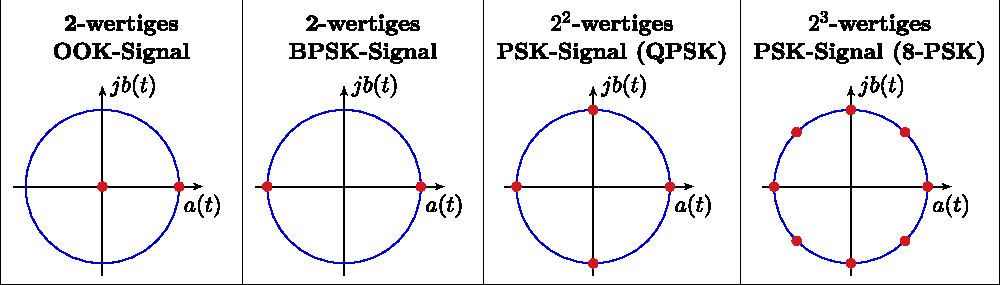
\includegraphics{content/08_digsigtransmit/basisbanddarstellungen.pdf}

\subsection{Quadratur Amplitudenmodulation (QAM) S. 118}
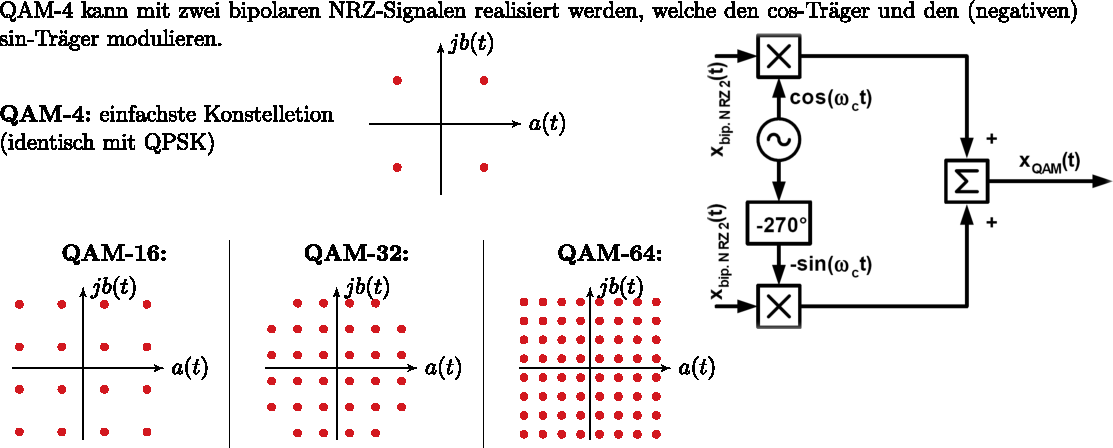
\includegraphics{content/08_digsigtransmit/qam.pdf}

Anzahl Bit pro Symbol $= floor(\log_2(\text{Anzahl Punkte}))$ \hspace{.5cm} \efbox[linecolor=red]{$B_{QAM-rc} = f_s(1+\alpha) \;\;\; |\;\; \alpha \text{ Roll-off Faktor}$}

\subsubsection{Gray-Codierung von QAM}
\begin{minipage}{.4\linewidth}
	Bitfehler entstehen, wenn bei beeinträchtigtem
	Empfang falsche Amplitudenwerte decodiert wer-
	den. Dabei ist es am Wahrscheinlichsten, dass ein
	benachbartes Feld detektiert wird.
	Durch den \textbf{Gray-Code} können \textbf{mehrfache Bit-
	fehler vermieden} werden (zwischen Nachbarn
	ändert nur 1 Bit).
\end{minipage}
\hspace{1cm}
\begin{minipage}{.6\linewidth}
	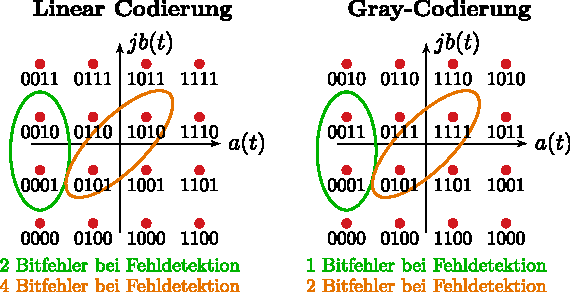
\includegraphics[width=.8\linewidth]{content/08_digsigtransmit/graycodeqam.pdf}
\end{minipage}

\subsubsection{Pulsformfilter zur QAM S. 121}
Rechteckige Signale im Basisband $\rightarrow$ hoher Bandbreitenbdarf im Basisband $\rightarrow$ doppelter Bandbreitenbedarf im Basisband!\\
Bandbreite im Basisband kann mit Pulsformfilter gezielt reduziert werden.\\
Geeigenter Filter: \textbf{Raised-Cosine Filter}

\paragraph{Gefilterte Übergänge}
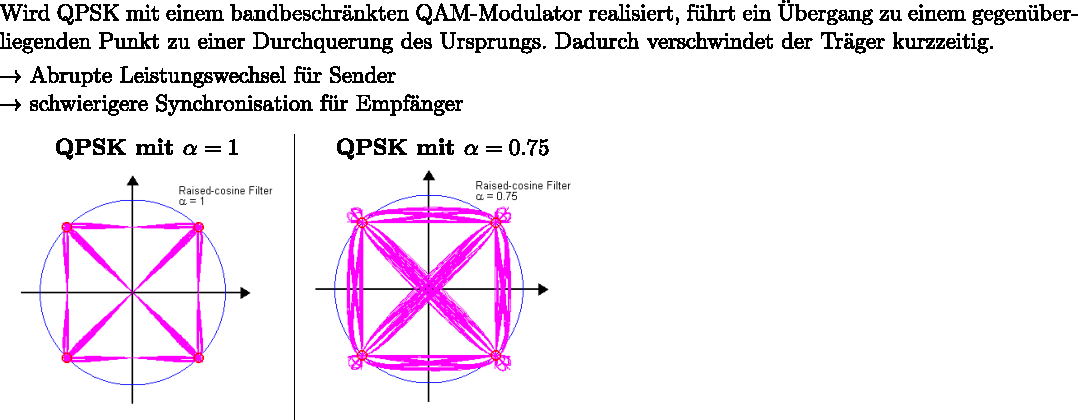
\includegraphics{content/08_digsigtransmit/gefilterteuebergaenge.pdf}

\paragraph{Filterung mit Offset}
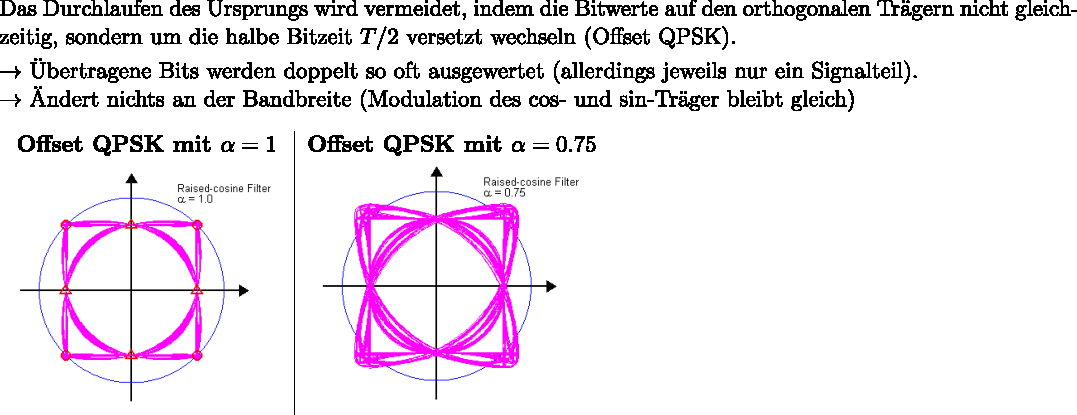
\includegraphics{content/08_digsigtransmit/filterungmitoffset.pdf}

	
	\begin{landscape}
		\section{Fancy Tabelle}
		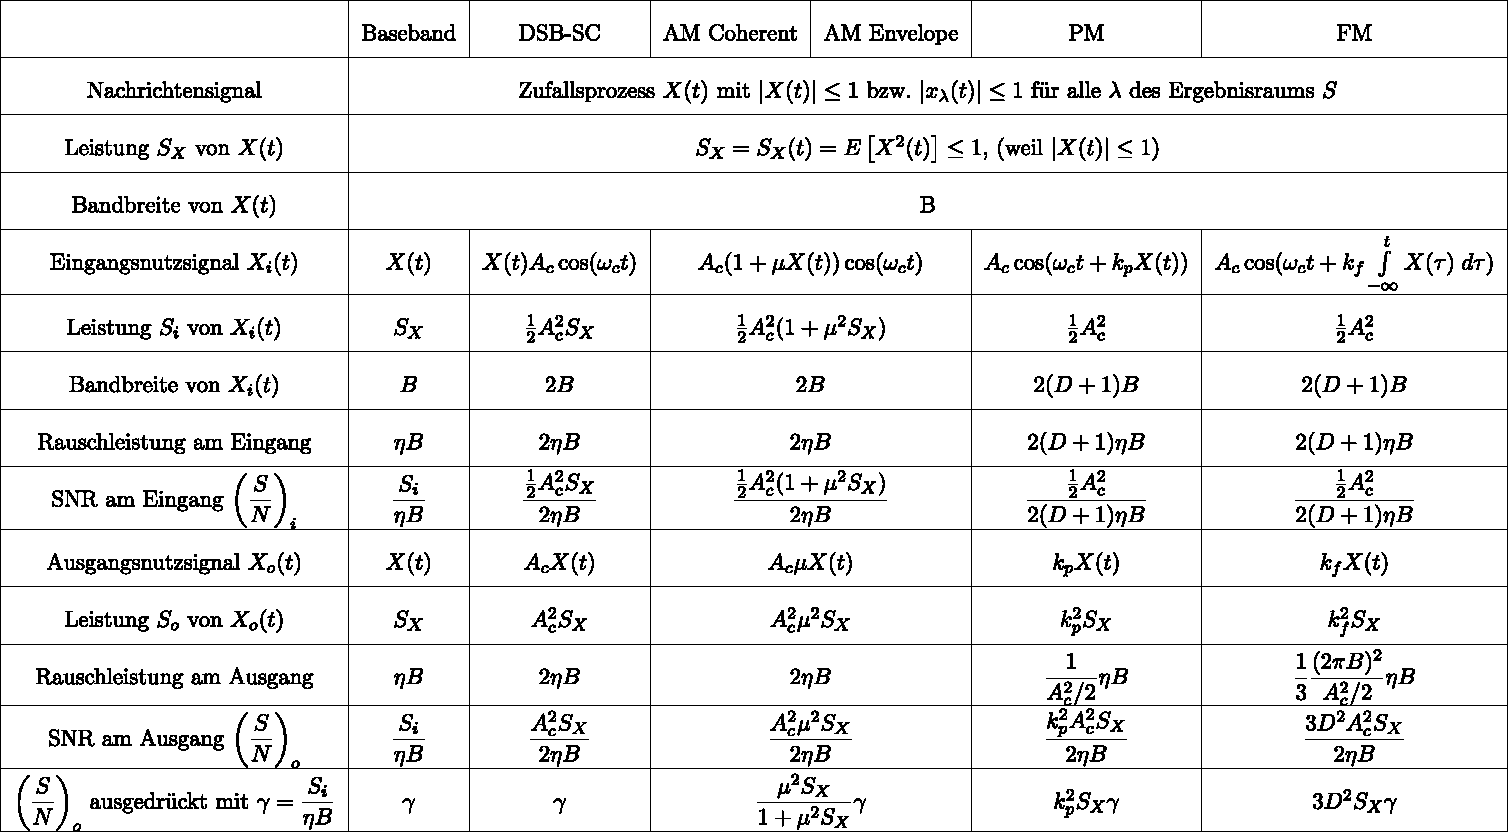
\includegraphics{content/fancytabelle.pdf}
	\end{landscape}

	\section{Idiotenseite}
	\begin{sidewaystable}
%\subsection{Eigenschaften unterschiedlicher Schwingungsformen}
\begin{center}
\begin{tabular}{|l|c|c|c|c|c|c|c|c|}
\hline
	Schwingungsform & Funktion & Gleichrichtwert & Formfaktor &
	Effektivwert & Scheitelfaktor & \textbf{$X_0$} & \textbf{$X^2$} & \textbf{var(X)} \\
\hline
	Formel &
	&
	$\overline{\left|x\right|} = \frac1T\int_{0}^{T}\left| x(t)\right|dt$&
	$\frac{X}{\overline{\left|x\right|}}$&
	$X = \sqrt{X^2} = \sqrt{\frac{1}{T} \int\limits ^{t_0+T}_{t_0}{x^2(t)dt}}$&
	$k_{s}=\frac{X_{\mathrm{max}}}{X_{\mathrm{eff}}}$&
	&
	&
	\\
\hline
	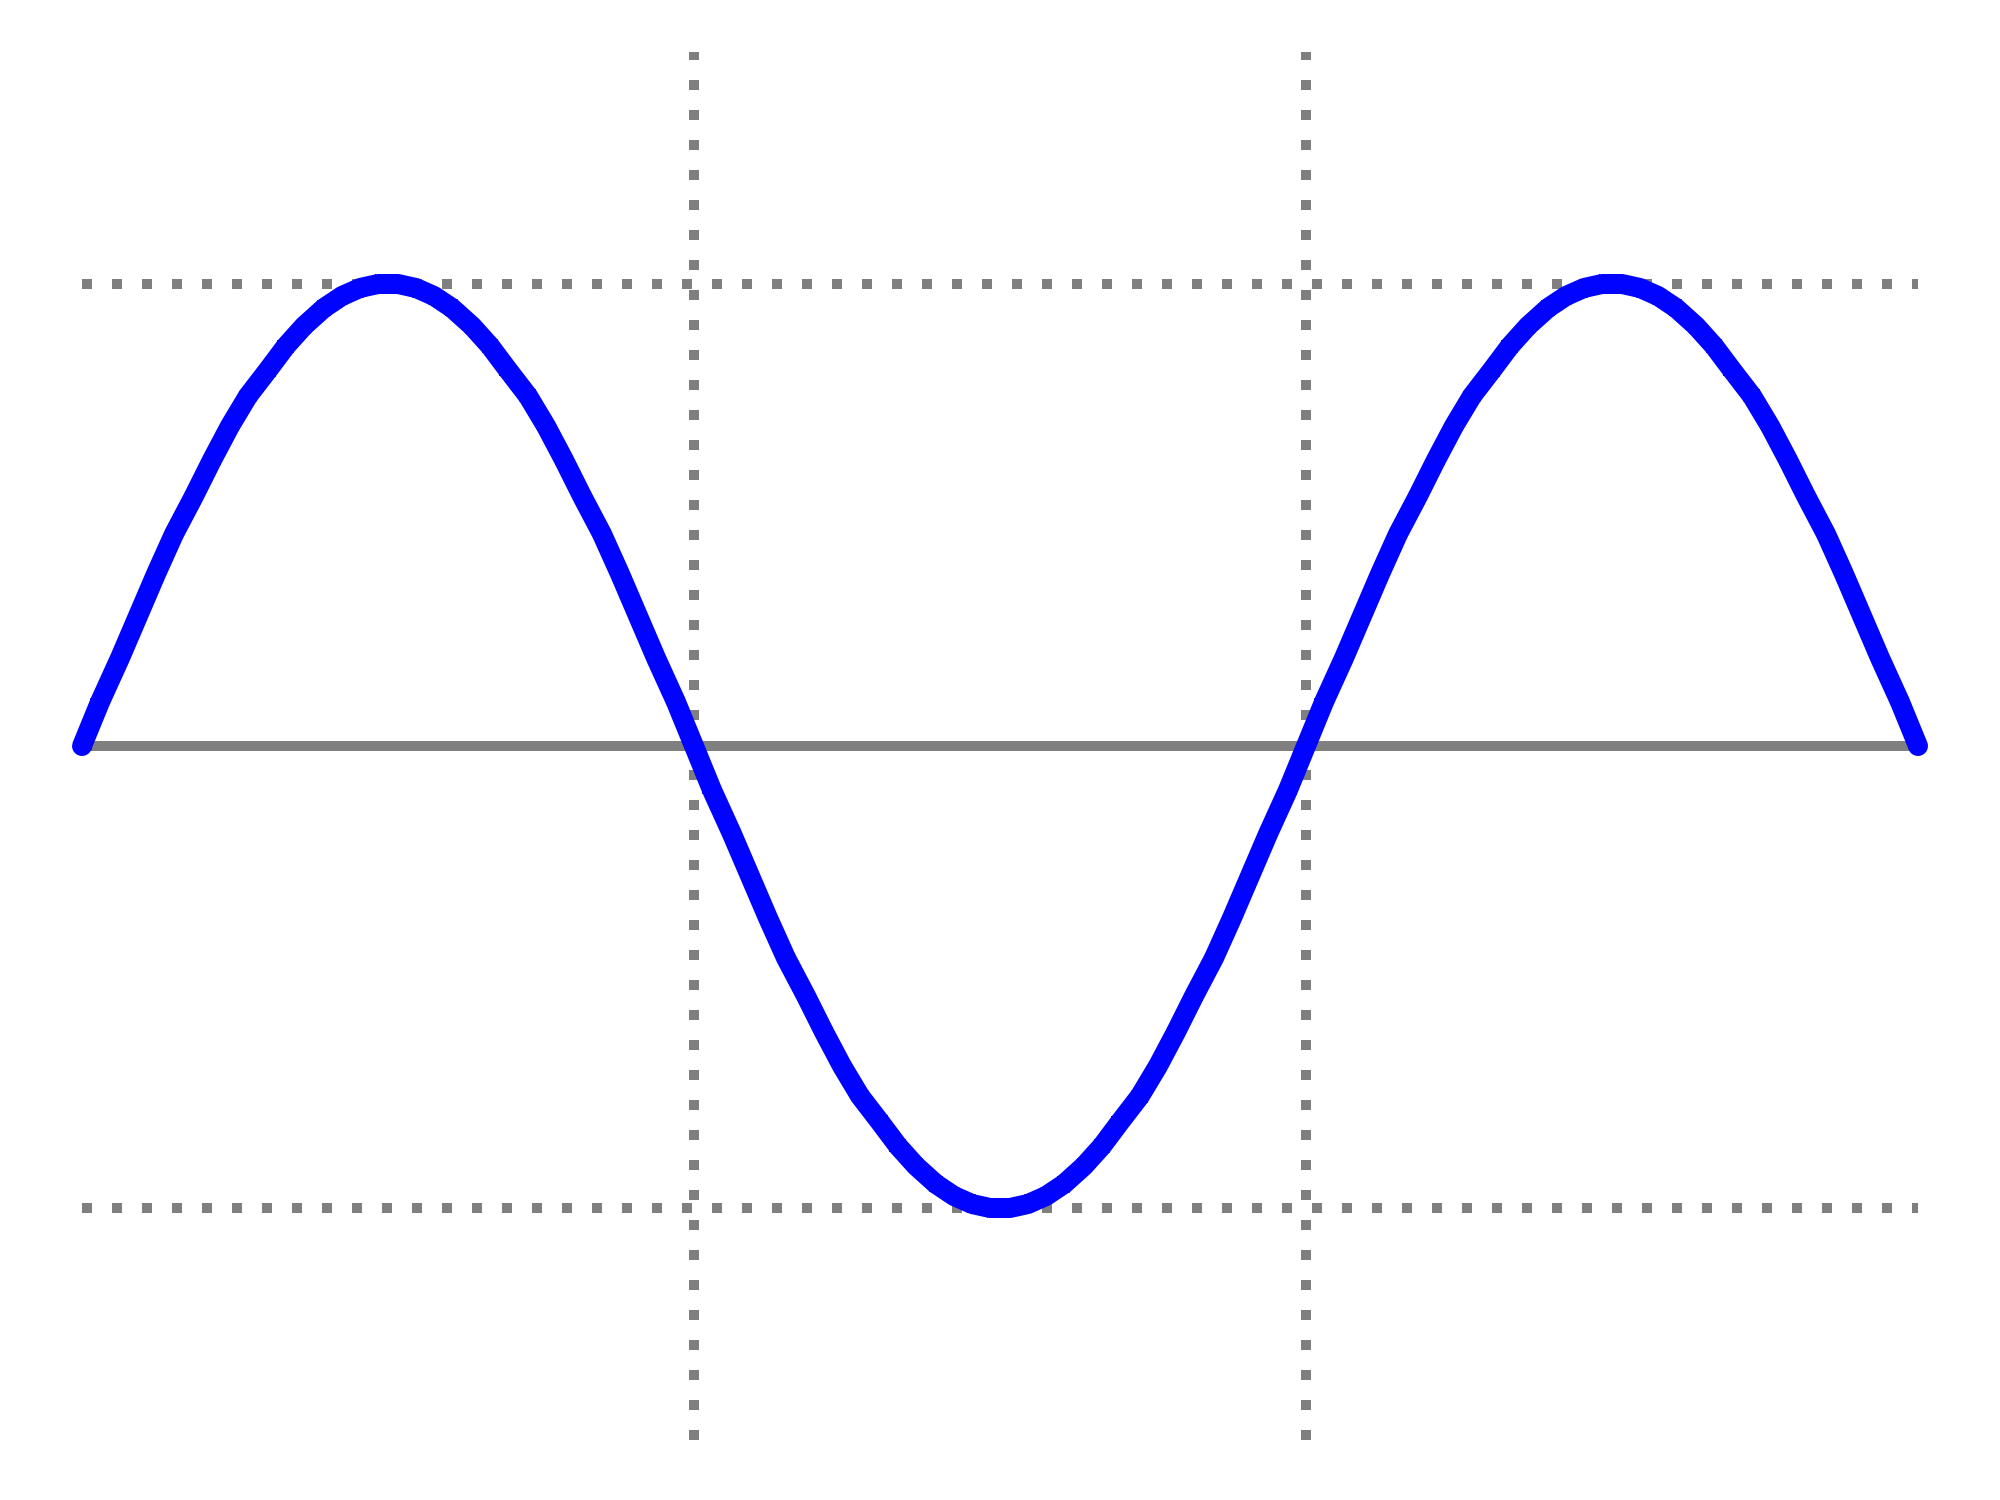
\includegraphics[width=2cm]{idiotenseite/images/table_sine_wave.png} &
	$A\cdot\sin(t)$ &
	$\frac{2}{\pi} \approx 0.637$ &
	$\frac{\pi}{2\sqrt{2}} \approx 1.11$ &
	$\frac{1}{\sqrt{2}}\approx 0.707$ &
	$\sqrt{2}\approx 1.414$ &
	$0$ &
	$\frac{A^2}{2}$ &
	$\frac{A^2}{2}$ \\
\hline	
	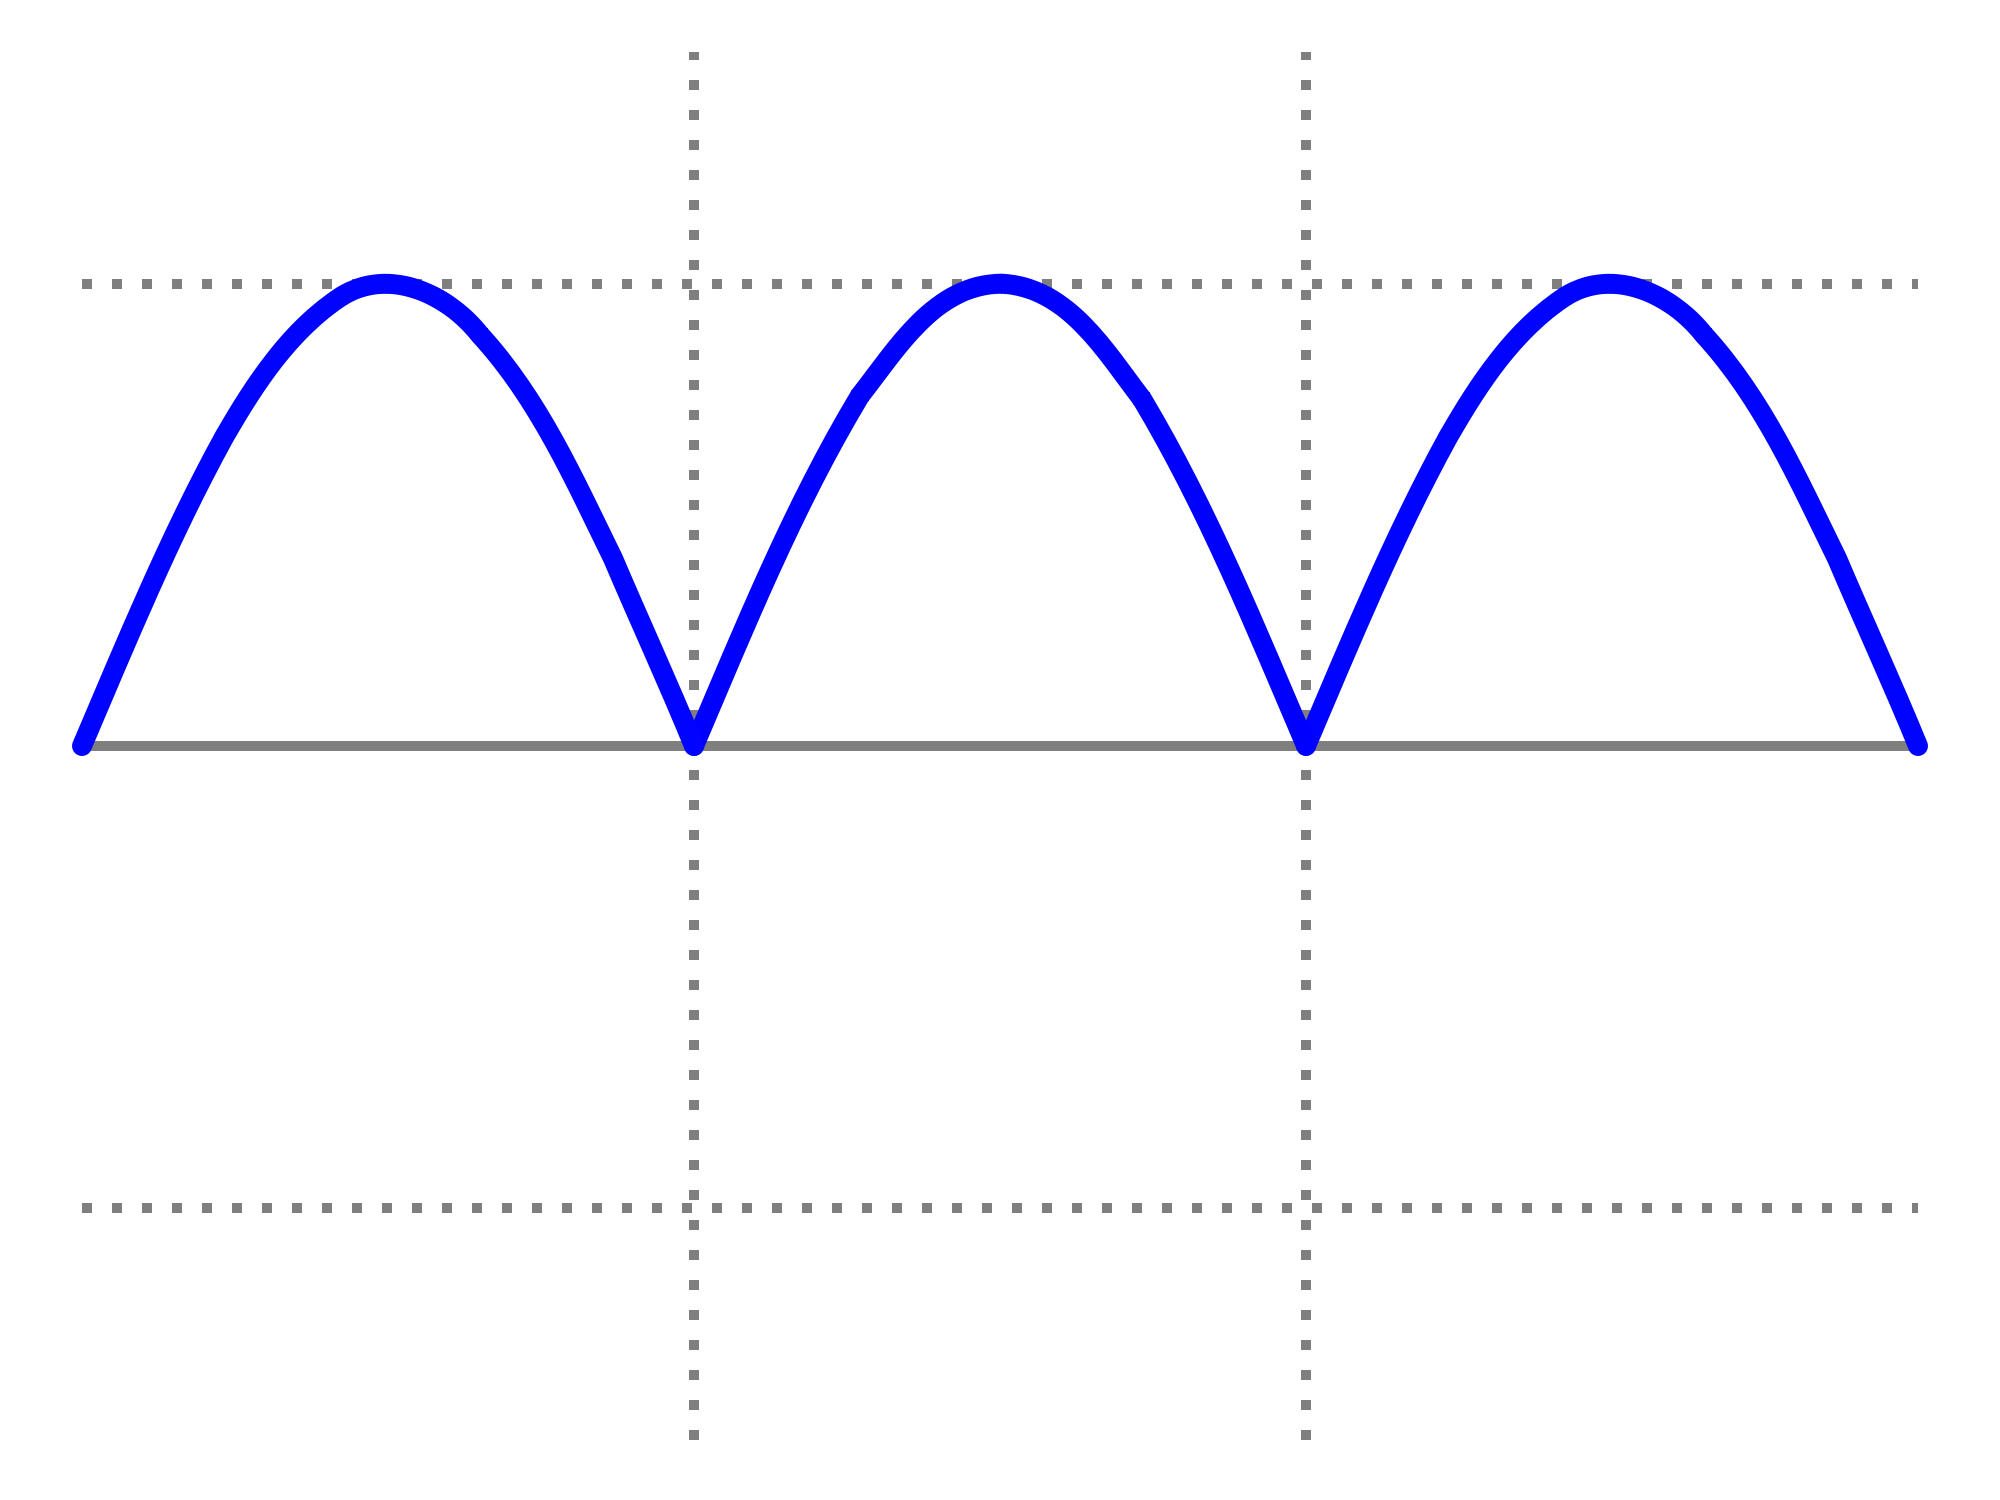
\includegraphics[width=2cm]{idiotenseite/images/table_full-wave_rectified_sine.png} &
	$A\cdot|\sin(t)|$ &
	$\frac{2}{\pi} \approx 0.637$ &
	$\frac{\pi}{2\sqrt{2}} \approx 1.11$ &
	$\frac{1}{\sqrt{2}} \approx 0.707$ &
	$\sqrt{2} \approx 1.414$  &
	$\frac{2A}{\pi}$ & $\frac{A^2}{2}$ & $\frac{A^2}{2}-\frac{4A^2}{\pi^2}$
	\\
\hline
	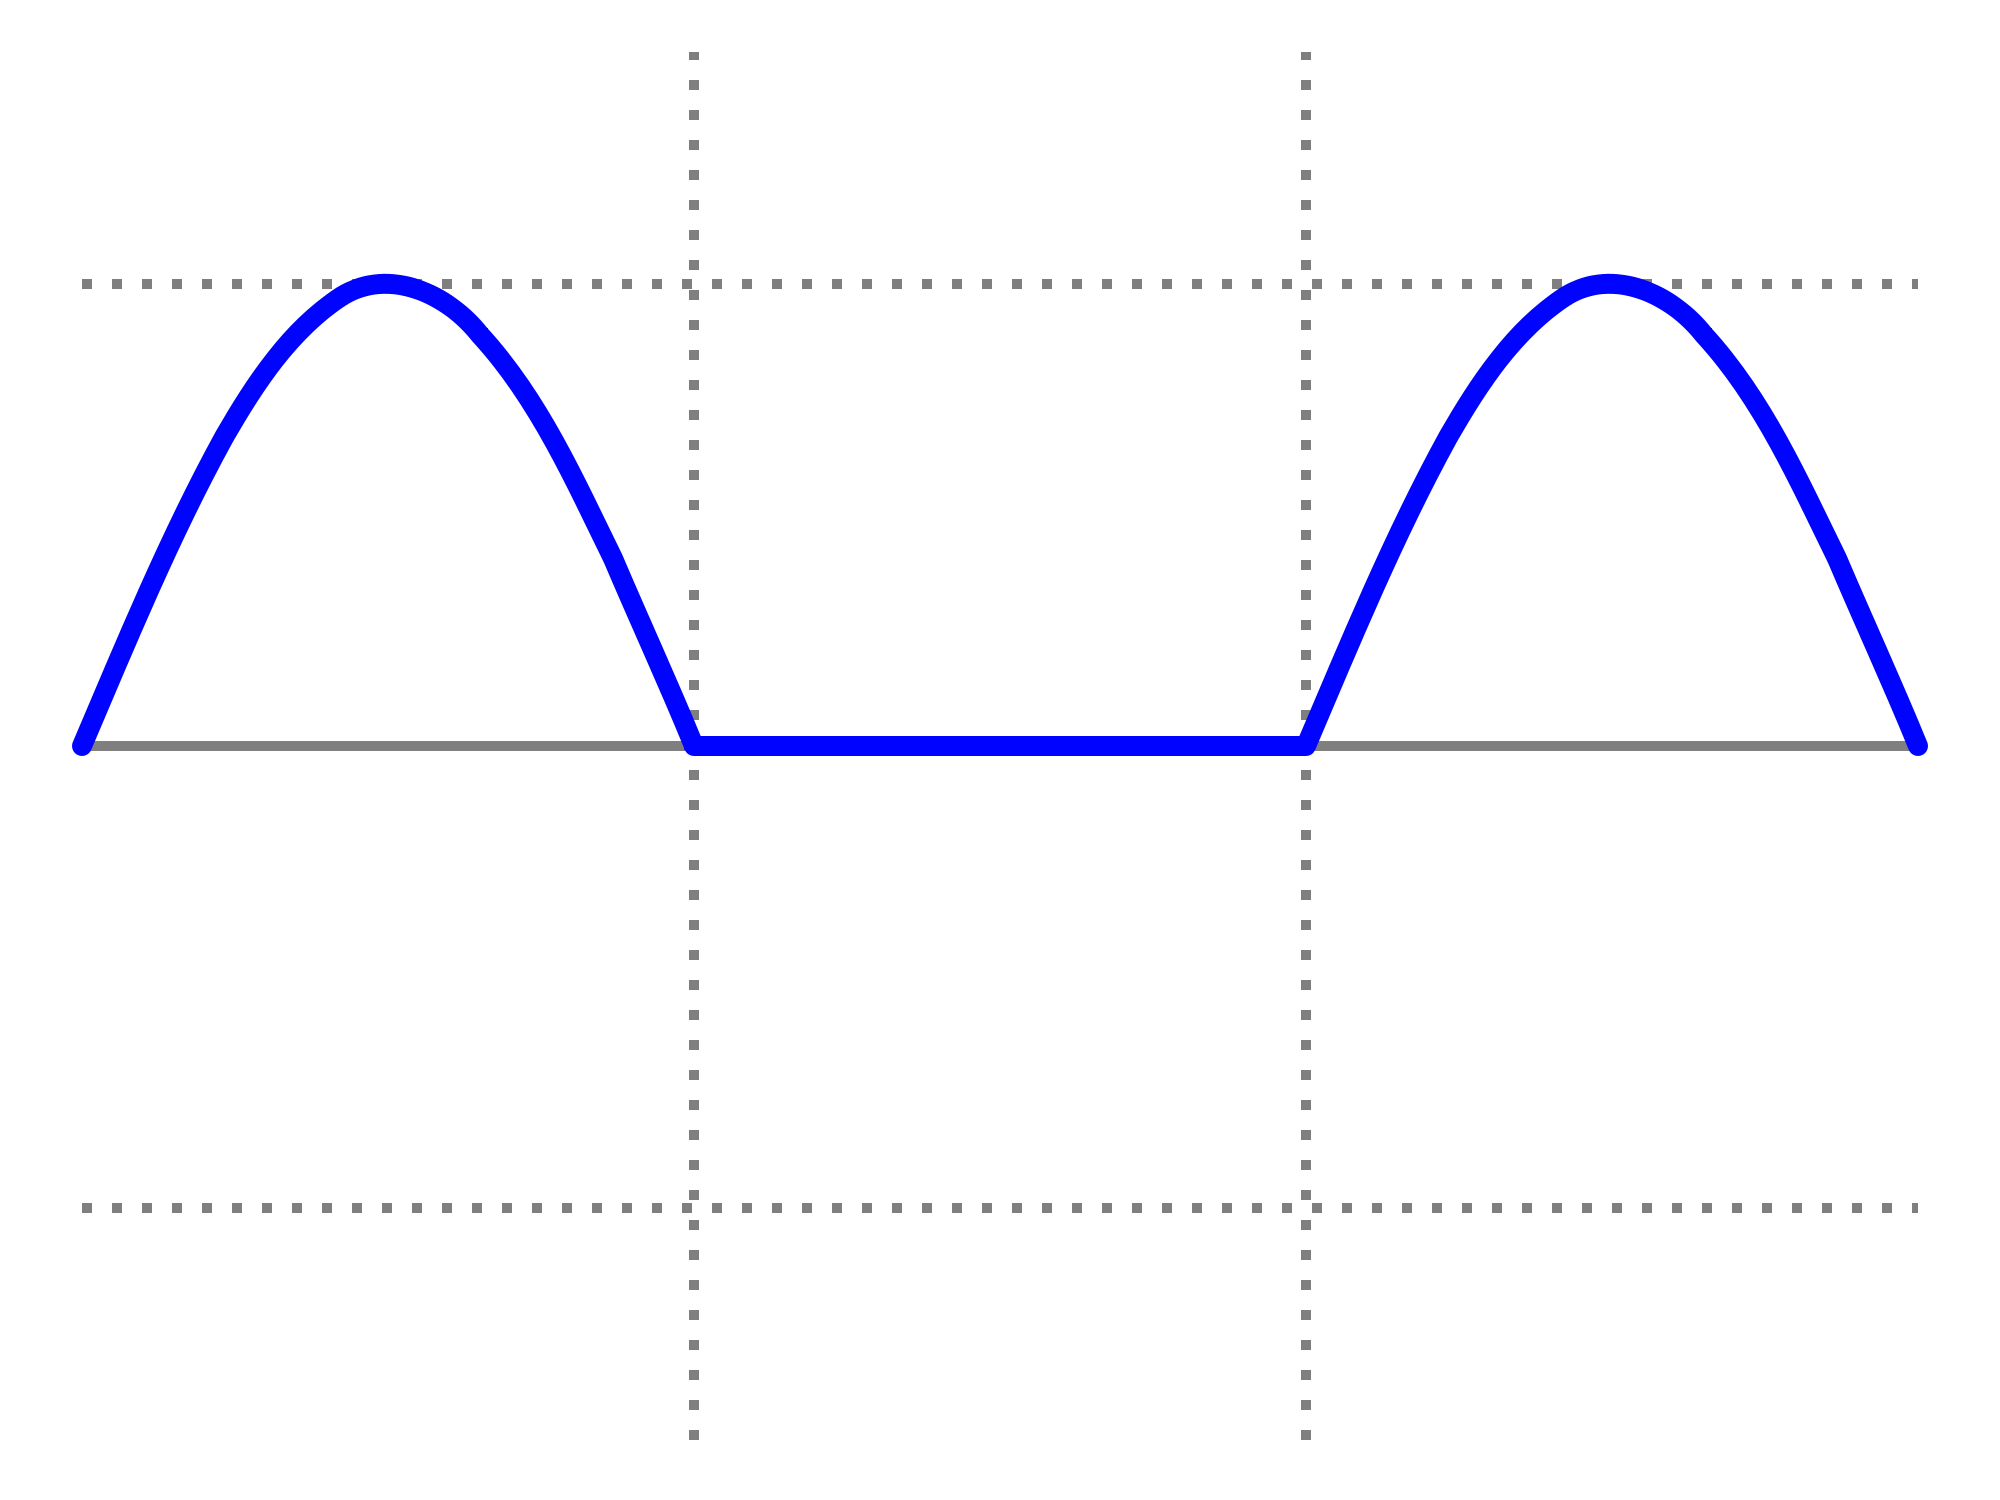
\includegraphics[width=2cm]{idiotenseite/images/table_half-wave_rectified_sine.png} &
	$\begin{cases} A\cdot\sin (t) & 0<t<\pi  \\ 0 & \text{True}\end{cases}$ &
	$\frac{1}{\pi}\approx 0.318$ &
	$\frac{\pi}{2}\approx 1.571$ &
	$\frac{1}{2} = 0.5$	&
	2  &
	$\frac{A}{\pi}$ &
	$\frac{A^2}{4}$ & $\frac{A^2}{4}-\frac{A^2}{\pi^2}$
	\\
\hline
	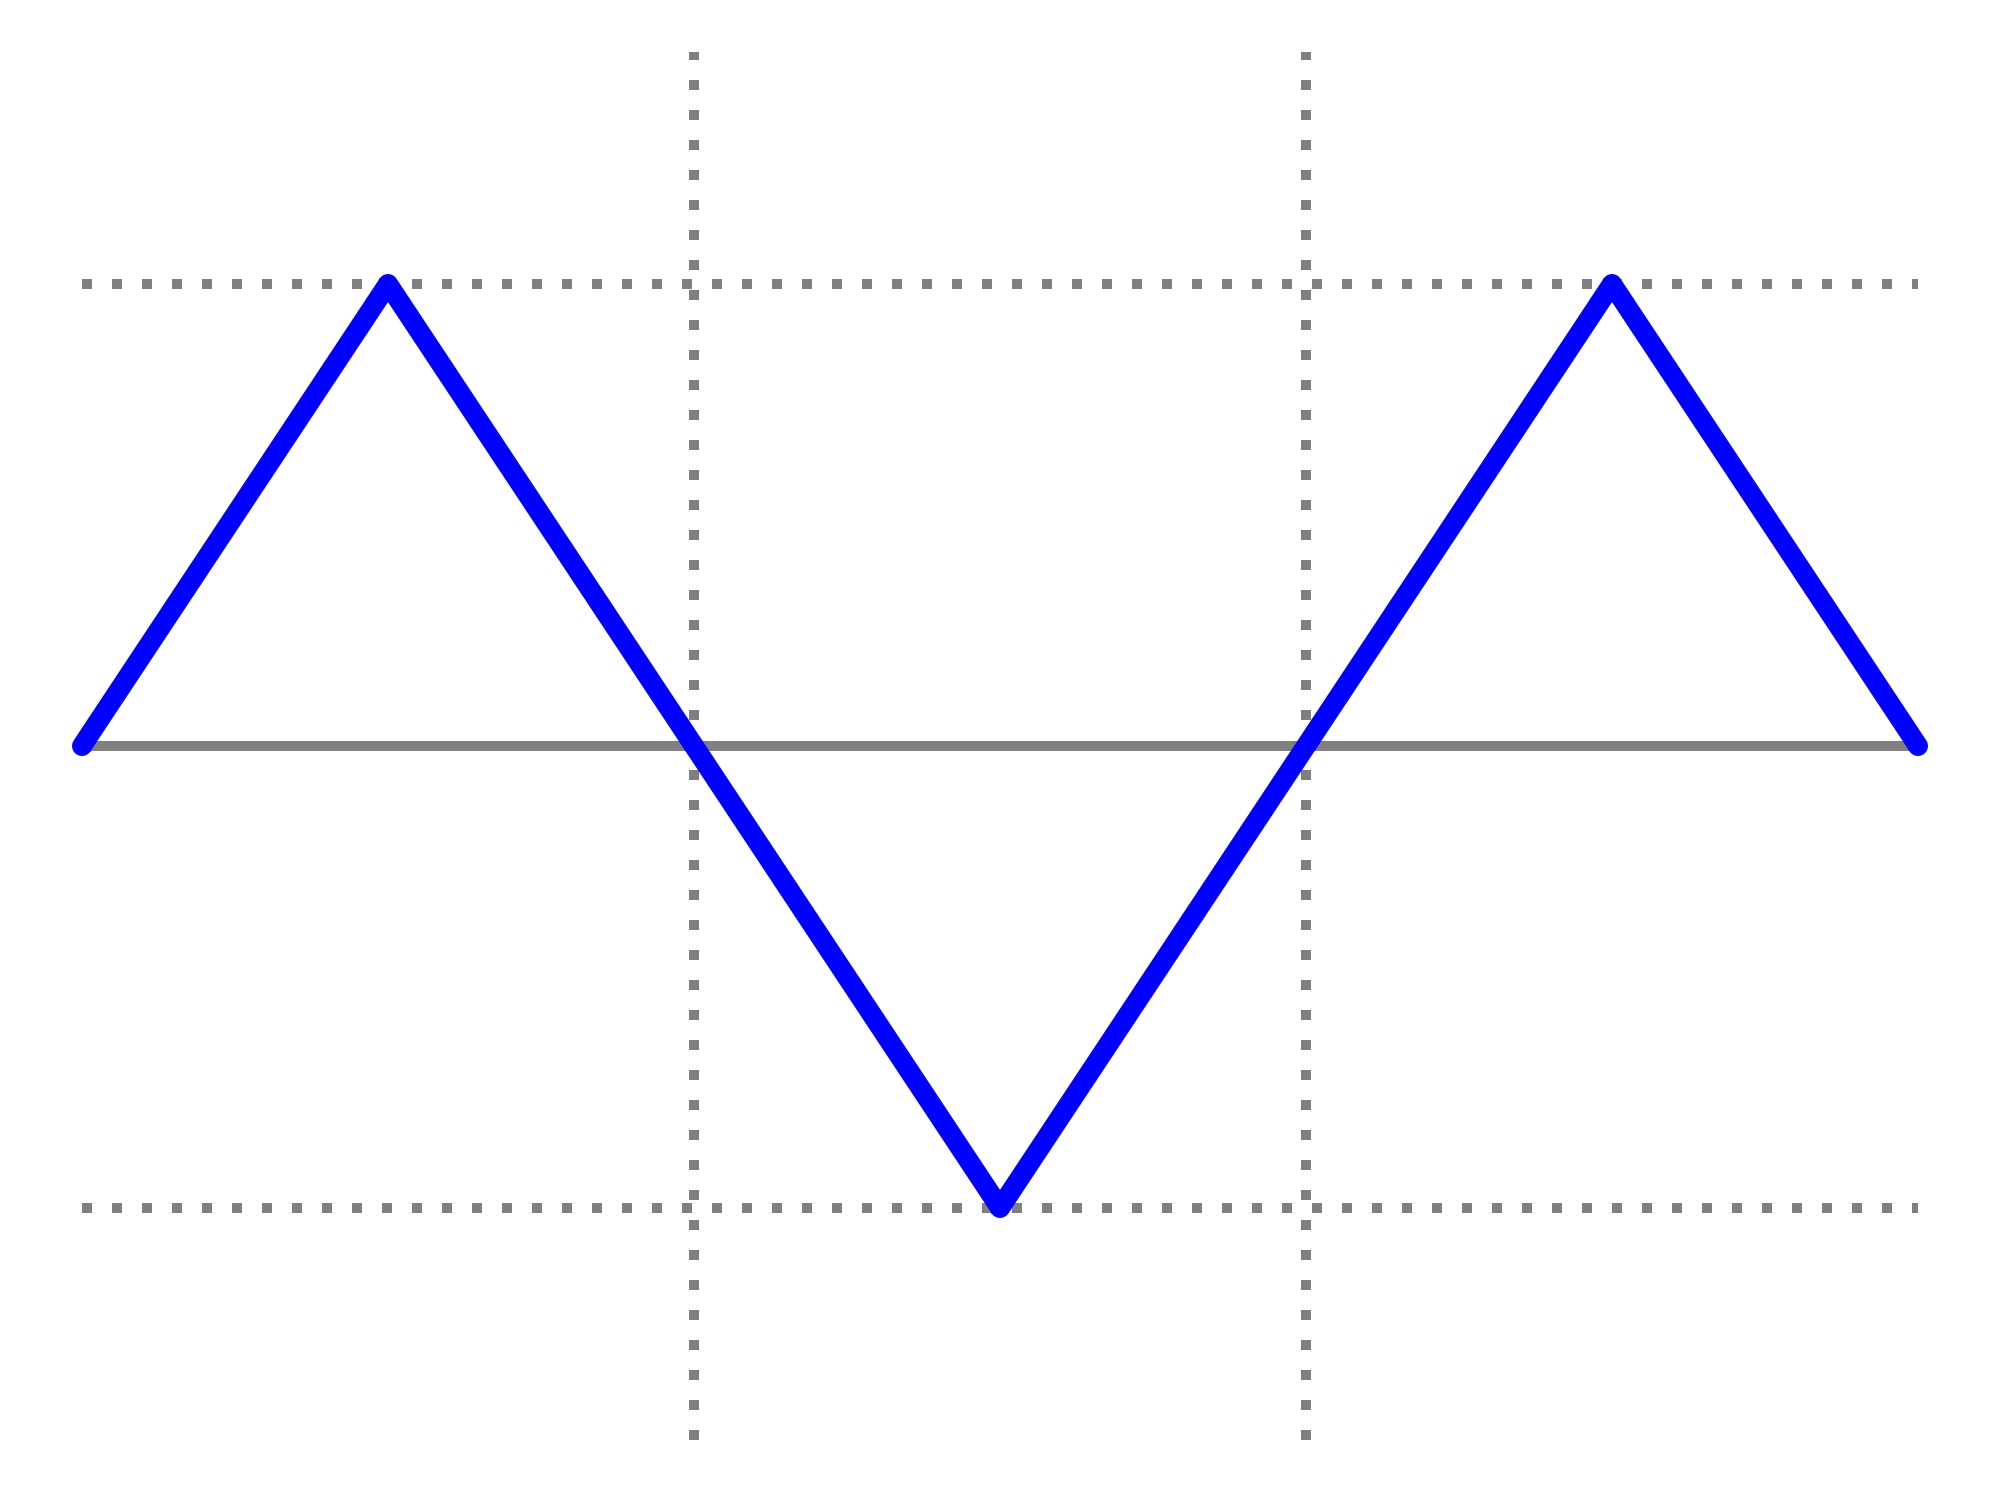
\includegraphics[width=2cm]{idiotenseite/images/table_triangle_wave.png} &
	$A\cdot\Lambda(t)$ &
	$\frac{1}{2}= 0.5$ &
	$\frac{2}{\sqrt{3}}\approx 1.155$ &
	$\frac{1}{\sqrt{3}}
	\approx 0.557$ &
	$\sqrt{3} \approx 1.732$ &
	$0$ &
	$\frac{A^2}{3}$ &
	$\frac{A^2}{3}$ \\
\hline	
	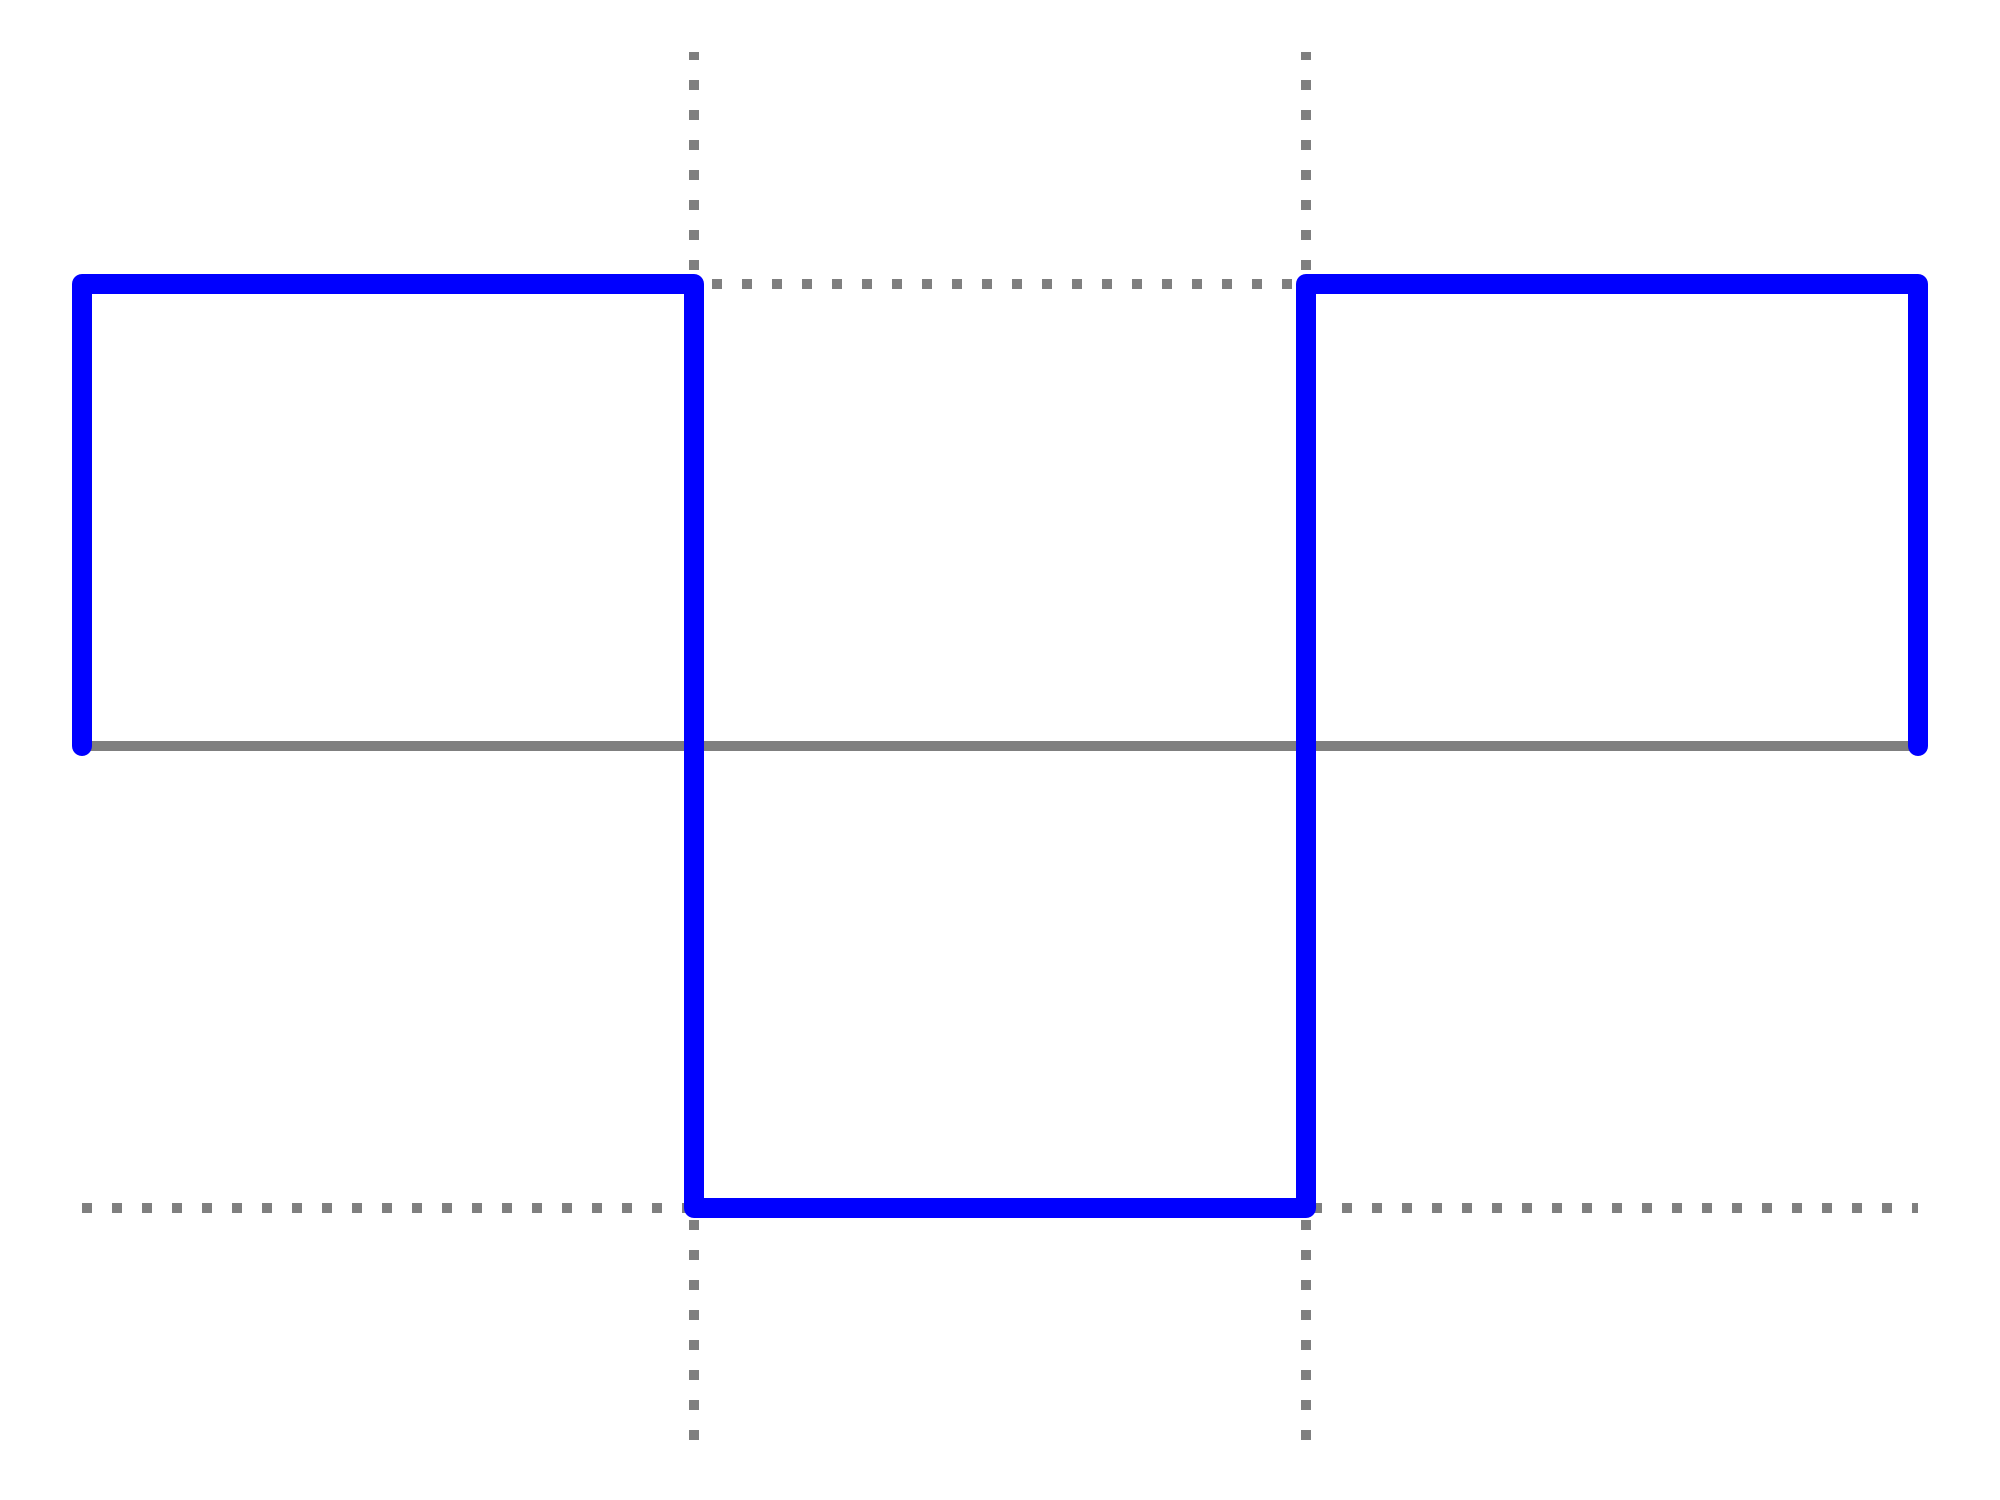
\includegraphics[width=2cm]{idiotenseite/images/table_square_wave.png} &
	$\begin{cases} A & 0<x<t \\ 0 & \text{True}\end{cases}$ &
	$1$ &
	$1$ &
	$1$ &
	$1$ &
	$0$ &
	$A^2$ &
	$A^2$ \\
\hline	
	DC&
	1&
	$1$ &
	$1$ &
	$1$ &
	$1$  &
	-&
	-&
	-\\
\hline	
	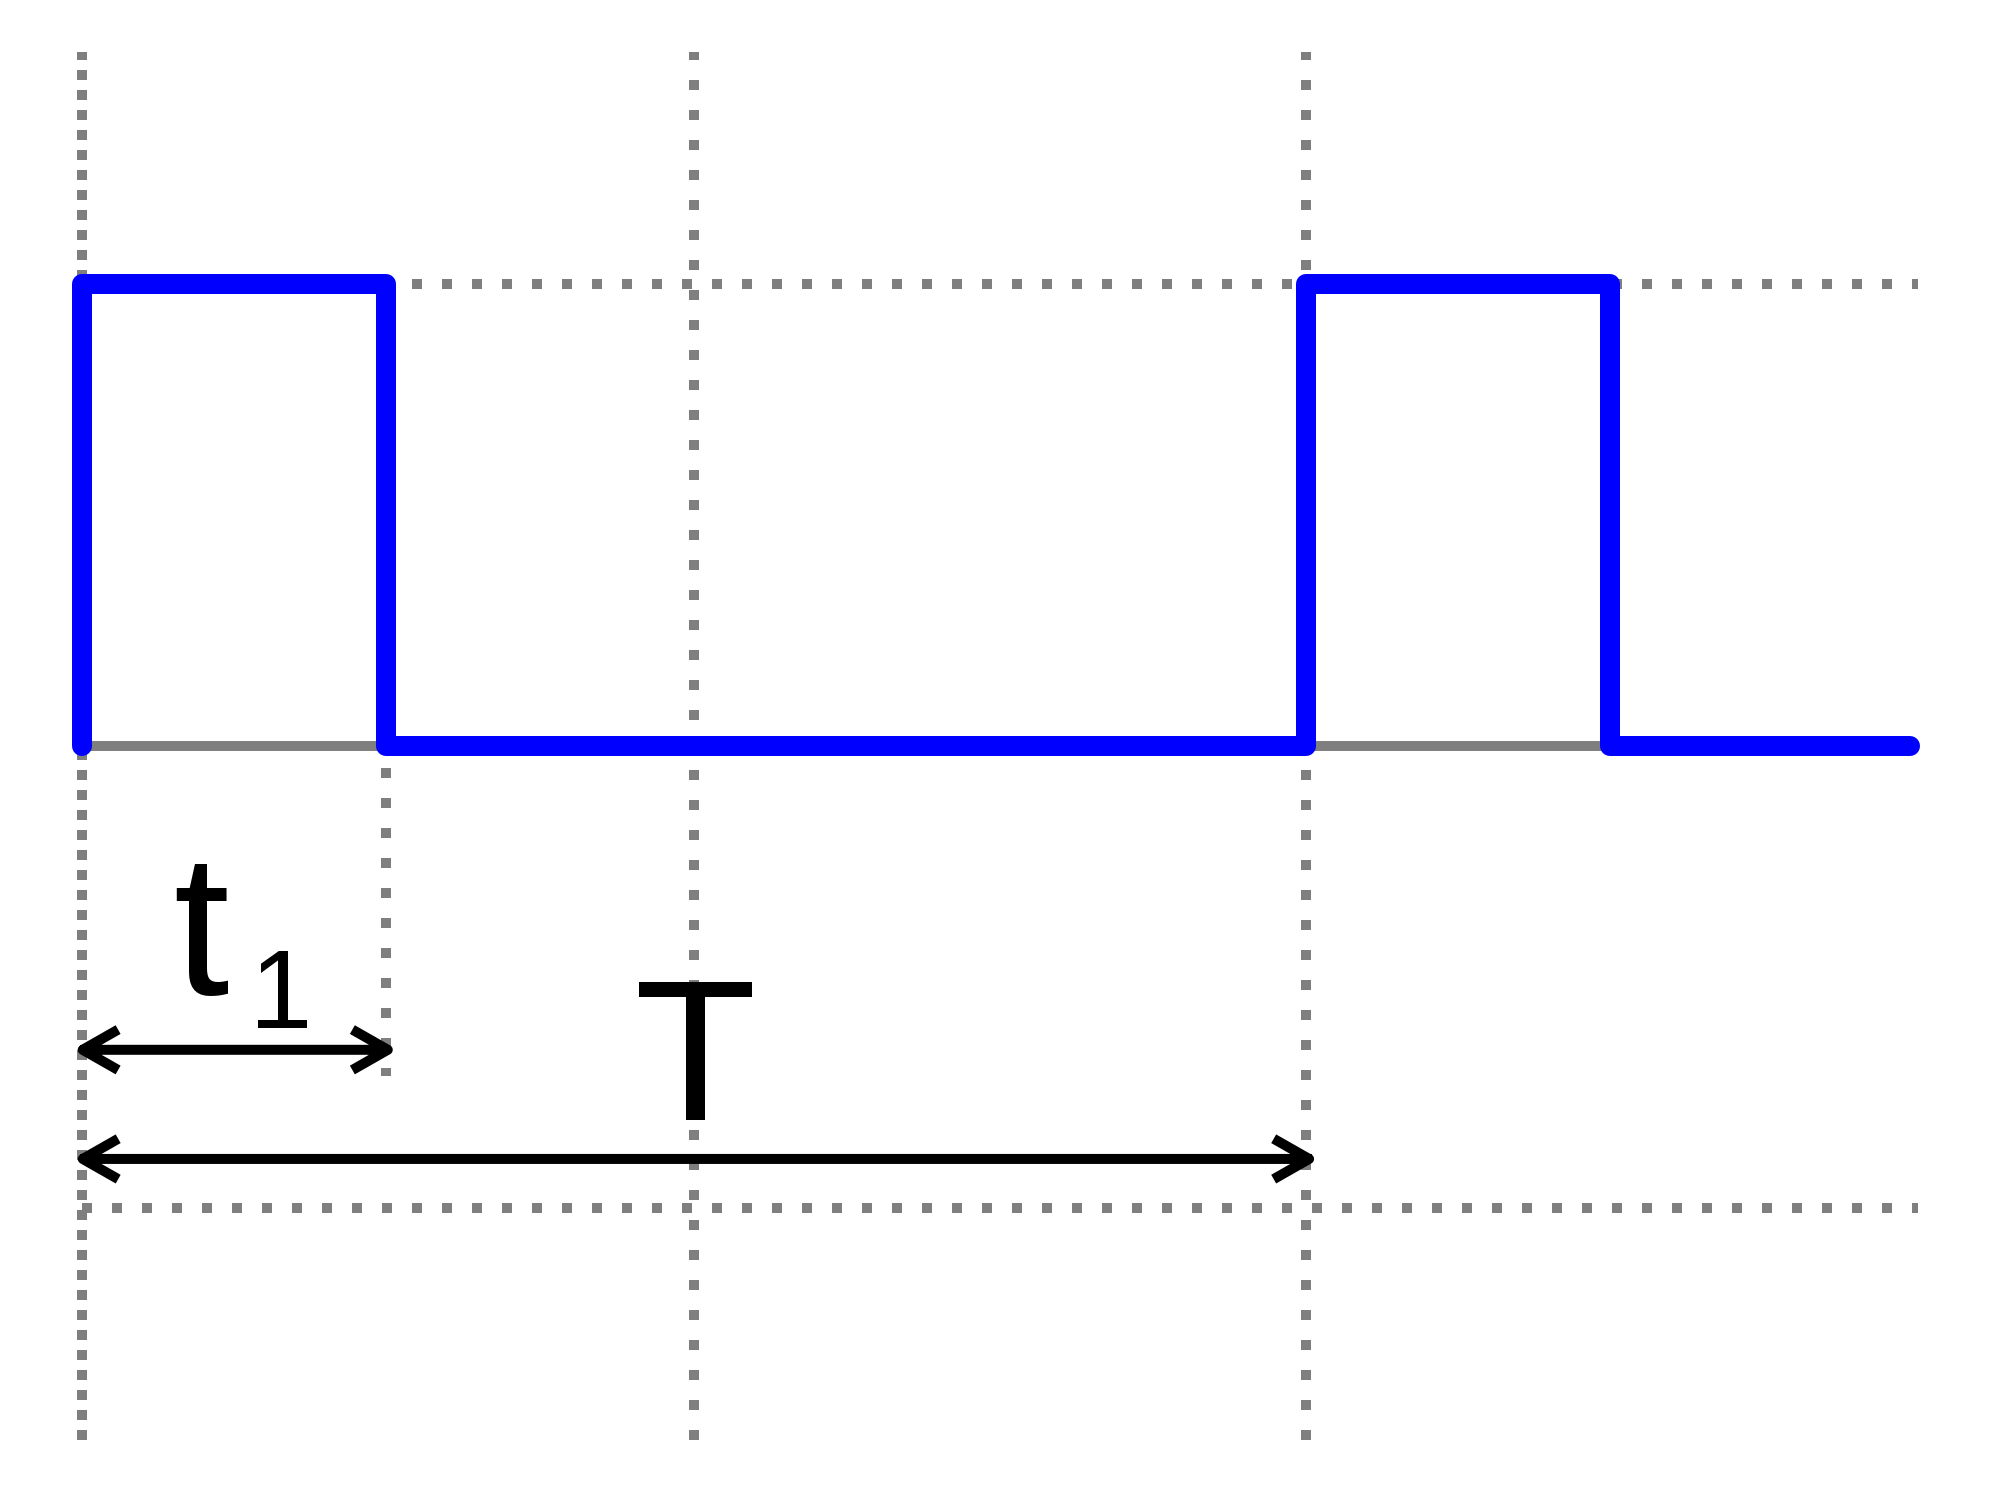
\includegraphics[width=2cm]{idiotenseite/images/table_pulse_wide_wave.png} &
	&
	$\frac{t_1}{T}$ & $\sqrt{\frac{T}{t_1}}$ & $\sqrt{\frac{t_1}{T}}$ & $\sqrt{\frac{T}{t_1}}$ &
	$A\frac{t}{T}$ &
	$A^2\frac{t}{T}$ &
	$\frac{A^2t}{T}-\frac{A^2t^2}{T^2}$\\
\hline
\end{tabular}
\end{center}
\end{sidewaystable}


	\subsection{Dreiecksformeln}
\begin{tabular}{lll}
	& \parbox{9.5cm}{
		\textbf{Cosinussatz} \\
		$$c^2 = a^2 + b^2 - 2 \cdot a \cdot b \cdot \cos \gamma$$\\
		\textbf{Sinussatz} \\
		$$\frac{a}{\sin \alpha} = \frac{b}{\sin \beta} = \frac{c}{\sin \gamma} = 2r =
		\frac{u}{\pi}$$
		\textbf{Pythagoras beim Sinus}\\
		$$\sin^2(b)+\cos^2(b)=1 \qquad \tan(b)=\frac{\sin(b)}{\cos(b)}$$}
		
	& \parbox{8cm}{
		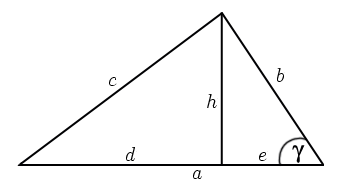
\includegraphics[width=6cm]{./idiotenseite/images/cosinussatz.png}}
\end{tabular}
\begin{center}
	\begin{multicols}{2}
		$\sin \beta = \frac ba =\frac{\text{Gegenkathete}}{\text{Hypotenuse}}$\\
		$\cos \beta = \frac ca =\frac{\text{Ankathete}}{\text{Hypotenuse}}$\\
		$\tan \beta = \frac cb =\frac{\text{Gegenkathete}}{\text{Ankathete}}$\\
		$\cot \beta = \frac cb =\frac{\text{Ankathete}}{\text{Gegenkathete}}$\\
	\end{multicols}
\end{center}

	
\subsection{Funktionswerte für Winkelargumente}
	\begin{minipage}{5cm}	
	\begin{tabular}[c]{|p{0.5cm}|p{0.4cm}||p{0.5cm}|p{0.5cm}|p{0.7cm}|}
	    	\hline
			deg & rad & sin & cos & tan$^-1$\\
			\hline
			0\symbol{23} & 0 & 0 & 1 & 0\\
			\hline
			30\symbol{23} & $\frac{\pi}{6}$ & $\frac{1}{2}$ & $\frac{\sqrt{3}}{2}$ &
			$\frac{1}{\sqrt{3}}$\\
			\hline
			45\symbol{23} & $\frac{\pi}{4}$ & $\frac{\sqrt{2}}{2}$ & $\frac{\sqrt{2}}{2}$
			& 1\\
			\hline
			60\symbol{23} & $\frac{\pi}{3}$ & $\frac{\sqrt{3}}{2}$ & $\frac{1}{2}$ &
			$\sqrt{3}$\\
			\hline			
	\end{tabular} \\
\end{minipage}
\begin{minipage}{14cm}
	\begin{multicols}{3}	
	\begin{tabular}[c]{|p{0.7cm}|p{0.7cm}||p{0.7cm}|p{0.7cm}|}
	    	\hline
			deg & rad & sin & cos\\
			\hline
			90\symbol{23} & $\frac{\pi}{2}$ & 1 & 0\\
			\hline	
			120\symbol{23} & $\frac{2\pi}{3}$ & $\frac{\sqrt{3}}{2}$ & $-\frac{1}{2}$ \\
			\hline
			135\symbol{23} & $\frac{3\pi}{4}$ & $\frac{\sqrt{2}}{2}$ & $-\frac{\sqrt{2}}{2}$\\
			\hline
			150\symbol{23} & $\frac{5\pi}{6}$ & $\frac{1}{2}$ & $-\frac{\sqrt{3}}{2}$\\
			\hline
	\end{tabular} \\
	
	\begin{tabular}[c]{|p{0.7cm}|p{0.7cm}||p{0.7cm}|p{0.7cm}|}
	  	\hline
		deg & rad & sin & cos\\
		\hline
		180\symbol{23} & $\pi$ & 0 & -1\\
		\hline	
		210\symbol{23} & $\frac{7\pi}{6}$ & $-\frac{1}{2}$ & $-\frac{\sqrt{3}}{2}$\\
		\hline
		225\symbol{23} & $\frac{5\pi}{4}$ & $-\frac{\sqrt{2}}{2}$ & $-\frac{\sqrt{2}}{2}$\\
		\hline
		240\symbol{23} & $\frac{4\pi}{3}$ & $-\frac{\sqrt{3}}{2}$ & $-\frac{1}{2}$\\
		\hline
	\end{tabular} \\
	
	\begin{tabular}[c]{|p{0.7cm}|p{0.7cm}||p{0.7cm}|p{0.7cm}|}
    	\hline
		deg & rad & sin & cos\\
		\hline
		270\symbol{23} & $\frac{3\pi}{2}$ & -1 & 0\\
		\hline	
		300\symbol{23} & $\frac{5\pi}{3}$ & $-\frac{\sqrt{3}}{2}$ & $\frac{1}{2}$\\
		\hline
		315\symbol{23} & $\frac{7\pi}{4}$ & $-\frac{\sqrt{2}}{2}$ & $\frac{\sqrt{2}}{2}$\\
		\hline
		330\symbol{23} & $\frac{11\pi}{6}$ & $-\frac{1}{2}$ & $\frac{\sqrt{3}}{2}$\\
		\hline
	\end{tabular}					
\end{multicols}
\end{minipage}

\begin{minipage}{13cm}
	\subsection{Periodizität}
	$\cos(a+k\cdot2\pi)=\cos(a) \qquad \sin(a+k\cdot2\pi)=\sin(a) \qquad
	(k \in \mathbb{Z})$
	\subsection{Quadrantenbeziehungen}
	\begin{tabbing}
    	xxxxxxxxxxxxxxxxxxxxxxxxxxxxxxxxxx \= \kill
	  	$\sin(-a)=-\sin(a)$ \> $\cos(-a)=\cos(a)$\\
		$\sin(\pi - a)=\sin(a)$ \> $\cos(\pi - a)=-\cos(a)$\\
		$\sin(\pi + a)=-\sin(a)$ \> $\cos(\pi +a)=-\cos(a)$\\
		$\sin\left(\frac{\pi}{2}-a \right)=\sin\left(\frac{\pi}{2}+a \right)=\cos(a)$ \>
		$\cos\left(\frac{\pi}{2}-a \right)=-\cos\left(\frac{\pi}{2}+a \right)=\sin(a)$  
    \end{tabbing}
\end{minipage}
\begin{minipage}{5cm}
	

\subsection{Ableitungen}

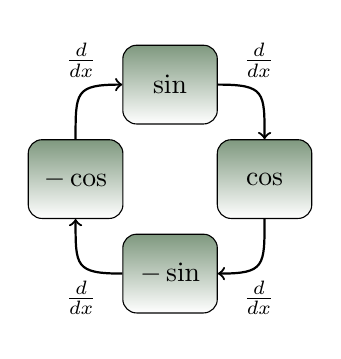
\begin{tikzpicture}
	[	inner sep = 2mm,
		sin/.style={rectangle,minimum width=1.2cm,minimum height=1cm,rounded corners=5pt,draw=black,top color=green!20!black!50},
		abl/.style={rectangle}
	]
	\node at (1.2,0) (sin1) [sin] {$\sin$};
	\node at (0,-1.2) (cos2) [sin] {$-\cos$};
	\node at (1.2,-2.4) (sin2) [sin] {$-\sin$};
	\node at (2.4,-1.2) (cos1) [sin] {$\cos$};
	
	\draw[thick,black,->] (sin1.east) .. controls +(right:0.6cm) and +(up:0.6cm) ..  (cos1.north)
	node [pos=0.5,above](abl) {$\frac{d}{dx}$};
	\draw[thick,black,->] (cos1.south) .. controls +(down:0.6cm) and +(right:0.6cm) .. (sin2.east)
	node [pos=0.5,below](abl) {$\frac{d}{dx}$};
	\draw[thick,black,->] (sin2.west) .. controls +(left:0.6cm) and +(down:0.6cm) .. (cos2.south)
	node [pos=0.5,below](abl) {$\frac{d}{dx}$};
	\draw[thick,black,->] (cos2.north) .. controls +(up:0.6cm) and +(left:0.6cm) .. (sin1.west)
	node [pos=0.5,above](abl) {$\frac{d}{dx}$};
\end{tikzpicture}
\end{minipage}
\begin{multicols}{2}
	\subsection{Additionstheoreme}
	$\sin(a \pm b)=\sin(a) \cdot \cos(b) \pm \cos(a) \cdot \sin(b)$\\
	$\cos(a \pm b)=\cos(a) \cdot \cos(b) \mp \sin(a) \cdot \sin(b)$\\	
	$\tan(a \pm b)=\dfrac{\tan(a) \pm \tan(b)}{1 \mp \tan(a) \cdot \tan(b)}$
	\columnbreak
	
	\subsection{Doppel- und Halbwinkel}	
	$\sin(2a)=2\sin(a)\cos(a)$\\
	$\cos(2a)=\cos^2(a)-\sin^2(a)=2\cos^2(a)-1=1-2\sin^2(a)$\\
	$\cos^2 \left(\frac{a}{2}\right)=\frac{1+\cos(a)}{2} \qquad
	\sin^2 \left(\dfrac{a}{2}\right)=\frac{1-\cos(a)}{2}$
\end{multicols}
\begin{multicols}{2}
	\subsection{Produkte}
		$\sin(a)\sin(b)=\frac{1}{2}(\cos(a-b)-\cos(a+b))$\\
		$\cos(a)\cos(b)=\frac{1}{2}(\cos(a-b)+\cos(a+b))$\\
		$\sin(a)\cos(b)=\frac{1}{2}(\sin(a-b)+\sin(a+b))$\\
	\subsection{Euler-Formeln} 

	$\sin(x) = \frac{1}{2j} \left(e^{jx} - e^{-jx}\right) \qquad
	\cos(x) = \frac{1}{2} \left(e^{jx} + e^{-jx}\right)$ \\
	$e^{x+jy} = e^x \cdot e^{jy} = e^x \cdot \left(\cos(y) + j\sin(y)\right)$ \\
	$e^{j\pi} = e^{-j\pi} = -1$ \\
	\columnbreak
	
	\subsection{Summe und Differenz}
		$\sin(a)+\sin(b)=2 \cdot \sin \left(\frac{a+b}{2}\right) \cdot
		\cos\left(\frac{a-b}{2}\right)$\\
		$\sin(a)-\sin(b)=2 \cdot \sin \left(\frac{a-b}{2}\right) \cdot
		\cos\left(\frac{a+b}{2}\right)$\\
		$\cos(a)+\cos(b)=2 \cdot \cos \left(\frac{a+b}{2}\right) \cdot
		\cos\left(\frac{a-b}{2}\right)$\\
		$\cos(a)-\cos(b)=-2 \cdot \sin \left(\frac{a+b}{2}\right) \cdot
		\sin\left(\frac{a-b}{2}\right)$\\
		$\tan(a) \pm \tan(b)=\dfrac{\sin(a \pm b)}{\cos(a)\cos(b)}$\\
\end{multicols}

	\newpage
\subsection{Kurven}
\begin{multicols}{4}
\subsubsection{e-Funktion}
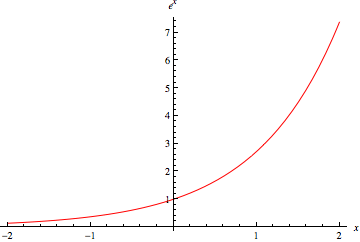
\includegraphics[width=4.5cm]{idiotenseite/images/Exp.png}
\subsubsection{Sinus-Funktion}
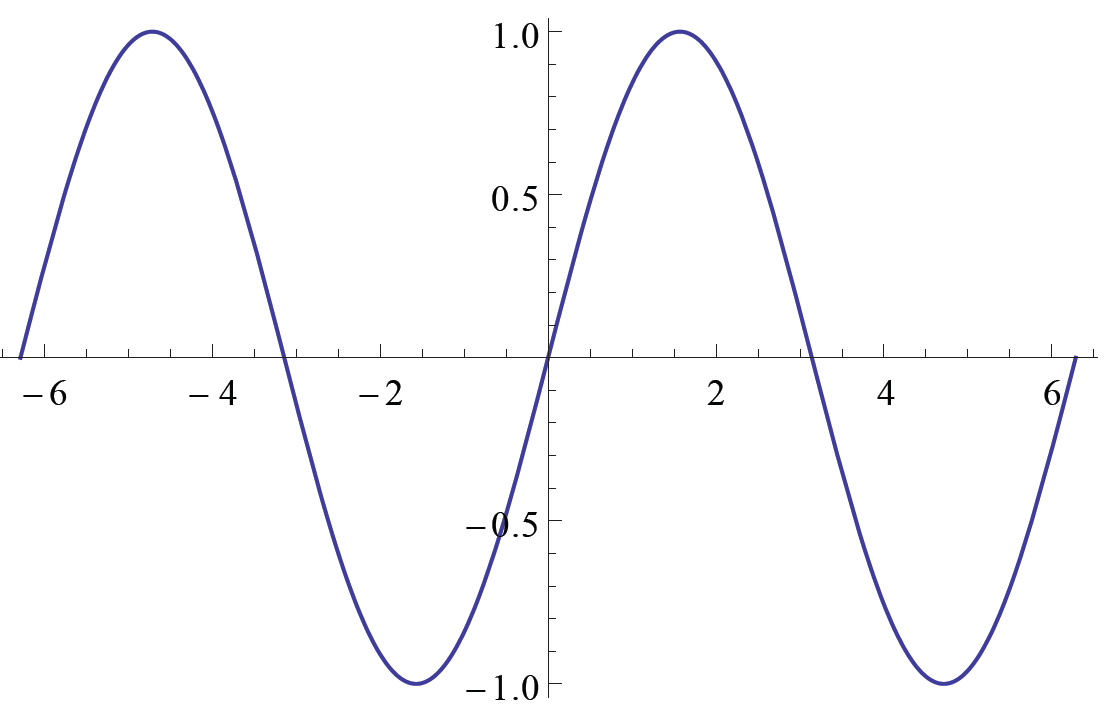
\includegraphics[width=4.5cm]{idiotenseite/images/sin.png}
\subsubsection{Cosinus-Funktion}
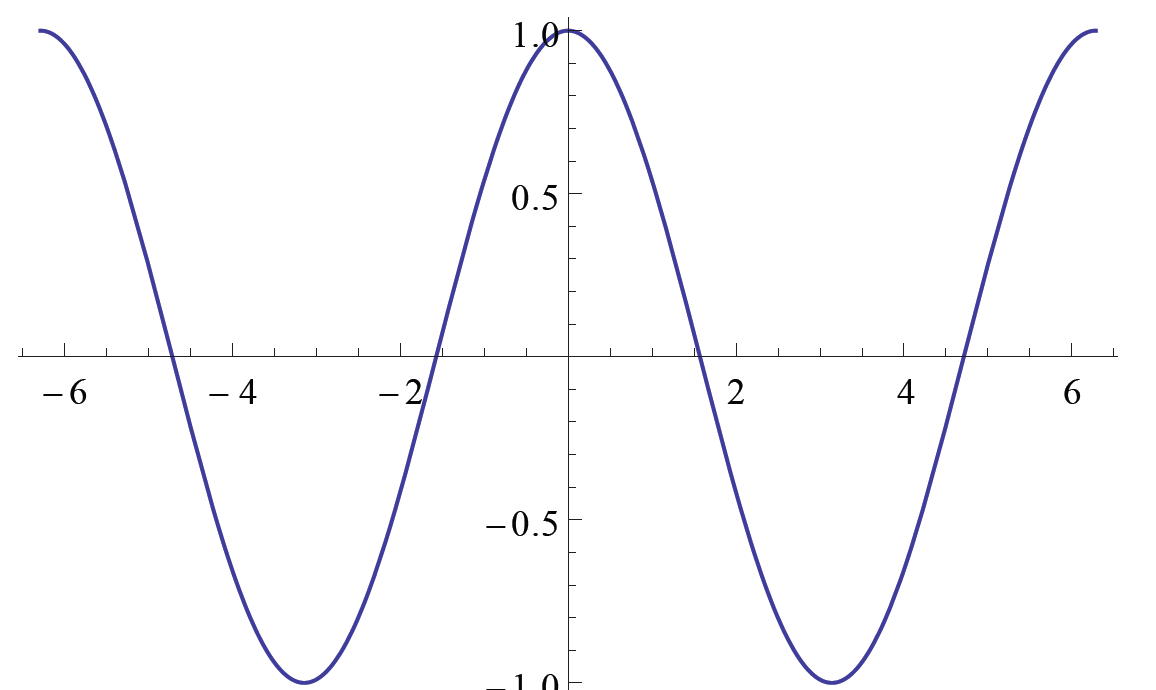
\includegraphics[width=4.5cm]{idiotenseite/images/cos.png}
\subsubsection{Tangens-Funktion}
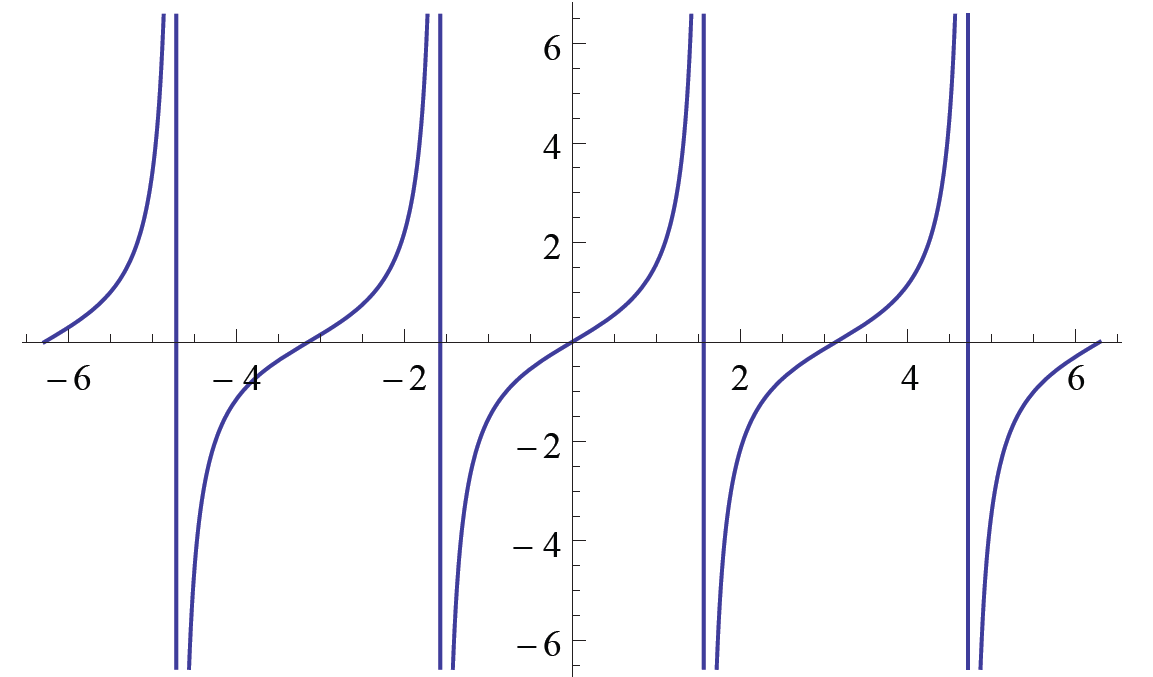
\includegraphics[width=4.5cm]{idiotenseite/images/tan.png}
\end{multicols}
	\subsection{Allgemein zeitabhängige Grössen}
	\begin{tabular}{|ll|ll|}
    \hline
	\multicolumn{2}{|l}{Arithmetischer Mittelwert, Gleichwert, Linearer MW} 
	    	& \multicolumn{2}{l|}{$X_0 = \overline{X} = X_m = \frac {1} {T} \int\limits_{t_0}^{t_0+T}
	    	x(t)dt$} \\
	\hline
	Quadratischer MW, Leistung 
		& $X^2 = \frac {1} {T} \int\limits_{t_0}^{t_0+T} x^2(t)dt$ 
		& MW $n$. Ordnung
		& $X^n = \frac {1} {T} \int\limits_{t_0}^{t_0+T} x^n(t)dt$ \\
	\hline
	Effektivwert (RMS) 
		& $X = \sqrt{X^2} = \sqrt{\frac{1}{T} \int\limits ^{t_0+T}_{t_0}{x^2(t)dt}}$
		& Gleichrichtwert 
		& $X_{|m|} = \bar{|X|} = \frac{1}{T} \int\limits_{t_0}^{t_0+T}{|x(t)| dt}$ \\
	\hline
\end{tabular}
	\section{Übungsverzeichnis}

\subsection{Einführung}
	\begin{tabular}{|p{9cm}|p{2.5cm}|p{3.5cm}|p{2cm}|}
	\hline
	\textbf{Thema} & \textbf{Hausübung} & \textbf{Schaum} & \textbf{Praktikum} \\
	\hline
	Dezibel & 1.2, 1.3, 1.4 &  &  \\
	\hline
	Fouriertransformierte & 2.1, 2.2, 2.4, 2.5 & 1.10, 1.14, 1.15, 1.28 &  \\
	\hline
	Komplexe Fourierreihe & 1.5, 1.6 & & \\
	\hline
	Modulationssatz & 2.3 & & \\
	\hline
	Crest-Faktor & 1.1 & & \\
	\hline
	\end{tabular}

\subsection{LTI-Systeme}
	\begin{tabular}{|p{9cm}|p{2.5cm}|p{3.5cm}|p{2cm}|}
	\hline
	\textbf{Thema} & \textbf{Hausübung} & \textbf{Schaum} & \textbf{Praktikum} \\ \hline
	LTI: Linearität und Zeitinvarianz & 2.6, 2.7 & 2.1, 2.2 &  \\ \hline
	LTI: RL-Filter & 3.1 & 2.11 &  \\ \hline
	\end{tabular}

\subsection{Amplitudenmodulation}
	\begin{tabular}{|p{9cm}|p{2.5cm}|p{3.5cm}|p{2cm}|}
	\hline
	\textbf{Thema} & \textbf{Hausübung} & \textbf{Schaum} & \textbf{Praktikum} \\ \hline
	DSB-SC &  & 3.1 - 3.3 & 3-6.2 \\ \hline
	OAM: Koharänte Demodulation & 4.1 & 3.5 & 4 \\ \hline
	OAM: Spitzenwertdetektor & 4.2 & 3.6 & 4 \\ \hline
	Ordinary AM & & 3.4 & 3 \\ \hline
	QAM & 5.3  & 3.15 & 4 \\ \hline
	SSB-AM: Demodulation mit koharäntem Demodulator & 5.2 & 3.9 & 4 \\
	\hline SSB-AM: Modulation mit Eintonsignal & 5.1 & 3.7, 3.8 & 4-7.2 \\ \hline
	Superheterodyne Empfänger & 4.3 & 3.13 & \\
	\hline
	\end{tabular}

\subsection{Winkelmodulation - FM/PM}
	\begin{tabular}{|p{9cm}|p{2.5cm}|p{3.5cm}|p{2cm}|}
	\hline
	\textbf{Thema} & \textbf{Hausübung} & \textbf{Schaum} & \textbf{Praktikum} \\ \hline
	FM/PM: Bandbreite & 7.2, 7.3 & 4.9, 4.10 & 5-7.3 \\ \hline
	FM/PM: Bandbreitenänderung & 7.5 & 4.13 & 5-7.3 \\ \hline
	FM/PM: Frequenz- \& Phasenabweichung & 6.4 & 4.2 & 5-7.1 \\ \hline
	FM/PM: Leistung des modulierten Signals & 7.1 & 4.6 &  \\ \hline
	FM/PM: Modulationsindex & 7.3, 7.4 & 4.10, 4.11, 4.12 &  \\ \hline
	FM/PM: Momentanfrequenz & 6.3 & 4.1 & 5-7.1 \\ \hline
	PM: Nichtlinearität & 6.2 & 4.4 &  \\ \hline
	FM Demodulation & 7.6 & & \\
	\hline
	\end{tabular}

\subsection{Digitale Übermittlung analoger Signale}
	\begin{tabular}{|p{9cm}|p{2.5cm}|p{3.5cm}|p{2cm}|}
	\hline
	\textbf{Thema} & \textbf{Hausübung} & \textbf{Schaum} & \textbf{Praktikum} \\ \hline
	Delta-Modulation & 10.1 & 5.21, 5.22, 5.23, 5.24 & 7 \\ \hline
	ISI, Pulse-Shaping (Raised Cosine) & 11.1 & 5.36 &  \\ \hline
	PCM: Quantisierungsrauschen, SNR & 9.4 & 5.15, 5.16 &  \\ \hline
	PCM: Samplerate, Quantisierung, Bitrate & 9.1 & 5.12 &  \\ \hline
	PCM: Samplerate, Wortbreite, Bitdauer & 9.3 & 5.14 &  \\ \hline
	PCM: SNR und Bitrate einer CD & 9.6 & 5.17 &  \\ \hline
	PCM: Wortbreite & 9.2, 9.5 & 5.13, 5.16 &  \\ \hline
	Quantisierung: Ungleichförmig: A-Law, $\mu$-Law; SNR & 9.7, 9.8 & 5.18, 5.19
	& 6 \\ \hline Sampling: Basisbandsignale & & 5.8 &  \\ \hline
	Sampling: Flat-top Sampling & 8.7 & 5.1 & 6 \\ \hline
	Sampling: Natural Sampling & 8.6 & 5.9 & 6 \\ \hline
	Sampling: Nyquist-Frequenz/-Rate/-Intervall & 8.3 & 5.6 &  \\ \hline
	Sampling: Subsampling & 8.4, 8.5 & 5.7, 5.8 &  \\ \hline
	Sampling: Unterabtastung & & 5.3 &  \\ \hline
	Leistungscodierung & 10.2 && \\ \hline
	Abtasttheorem & 8.2 & & \\ \hline
	Fax & 12.1 & & \\ \hline
	\end{tabular}

	\section{Prüfungsverzeichnis}

\begin{tabular}{|l|l|}
	\hline
	\textbf{Thema} & \textbf{Prüfung (Aufgabe)}\\
	\hline
	A/D Wandlung & 28.08.09 (3)\\
	\hline
	Amplitudenmodulation & 27.01.09 (1) \\
	\hline
	Basisbandübertragung von digitalen Signalen & 27.01.09 (4)\\
	\hline
	D/A Wandlung & 27.01.09 (3)\\
	\hline
	Digitale Basisbandübertragung & 02.02.10 (3)\\
	\hline
	Digitale Datenübertragung & 01.02.11 (4)\\
	\hline
	Digitale Signalübertragung mit moduliertem Träger & 02.02.10 (4)\\
	\hline
	Digitalisierung & 01.02.11 (3)\\
	\hline
	Digitalisierung & 02.02.10 (2)\\
	\hline
	DSB-SC, SSB und QAM & 02.02.10 (1)\\
	\hline
	Modulation & 01.02.11 (1)\\
	\hline
	OOK und PSK & 28.08.09 (4)\\
	\hline
	Phasenmodulation & 28.08.09 (1)\\
	\hline
	Übertragung zweier modulierter Trägersignale & 28.08.09 (2)\\
	\hline
	Winkelmodulation & 01.02.11 (2)\\
	\hline
	Winkelmodulation & 27.01.09 (2)\\
	\hline
\end{tabular}
	
	

\end{document}